\documentclass{sapientia-thesis}

% ── Bibliography file ────────────────────────────────────────────────────────
\thesisbibfile{references.bib}

% ── Student-specific metadata ────────────────────────────────────────────────
\titleRO{Recunoașterea automată a instrumentelor muzicale pe baza înregistrărilor audio}
\titleHU{Automatikus hangszerfelismerés zenefelvételek alapján}
\titleEN{Automatic Musical Instrument Recognition Based on Audio Recordings}
\studentname{Nagy Csaba}
\yearofthesis{2026}

\programro{SPECIALIZAREA CALCULATOARE}
\programhu{SZÁMÍTÁSTECHNIKA SZAK}
\programen{COMPUTER SCIENCE}

\supervisorRO{%
  \textbf{Conf.\ univ.\ dr.\ Iclănzan David Andrei}%
}

\supervisorHU{%
  \textbf{Dr.\ Iclănzan David Andrei, egyetemi docens}%
}

\supervisorEN{%
  \textbf{Assoc.\ Prof.\ Dr.\ Iclănzan David Andrei}%
}\usepackage{indentfirst}
\usepackage{amssymb}
\usepackage{pgfplots}
\pgfplotsset{compat=1.18}
\usepgfplotslibrary{groupplots}
\usetikzlibrary{positioning}
\usepackage{xcolor}
\usepackage{listings}
\usepackage{newunicodechar}
\usepackage{float}
\newunicodechar{█}{\rule{0.5em}{1.4ex}}
\newunicodechar{░}{{\color{lightgray}\rule{0.5em}{1.4ex}}}
\lstset{
  basicstyle=\ttfamily\small,
  literate={█}{{\rule{0.5em}{1.4ex}}}1 {░}{{\color{lightgray}\rule{0.5em}{1.4ex}}}1,
  keepspaces=true,
  breaklines=true
}

\makeatletter
\@addtoreset{figure}{section}
\@addtoreset{table}{section}
\makeatother
\renewcommand{\thefigure}{\thesection.\arabic{figure}}
\renewcommand{\thetable}{\thesection.\arabic{table}}


\begin{document}

% ════════════════════════════════════════════════════════════════════════════
% FRONT MATTER  (page order from the github version)
% ════════════════════════════════════════════════════════════════════════════
\pagenumbering{gobble}

% ── Page 1: Romanian cover page (LaTeX-generated) ────────────────────────────
\maketitlepagero

% ── Page 2: Assignment sheet (lucrare de diplomă / feladatkiírás) ─────────────
\includepdf[pages={2}]{Nagy_Csaba.pdf}

% ── Page 3: Declaration (declarație / nyilatkozat) ───────────────────────────
\includepdf[pages={3}]{Nagy_Csaba.pdf}

% ── Page 4: Romanian abstract / Extras ───────────────────────────────────────
\pagenumbering{roman}
\abstractpagero{Extras}{%
  Prezenta lucrare de diplomă abordează problema recunoașterii automate a
  instrumentelor muzicale pe baza înregistrărilor audio, utilizând metode
  moderne de învățare automată. Sistemul dezvoltat este capabil să clasifice
  în timp real șapte categorii de instrumente (chitară, pian, voce,
  instrumente cu coarde, instrumente cu ancie, instrumente de alamă și
  zgomot ambiental) pornind de la semnale audio monofonice.

  Abordarea propusă se bazează pe extragerea a trei tipuri de caracteristici
  spectrale (Log-Mel spectrograme, STFT și MFCC) și pe antrenarea unor rețele
  neuronale convoluționale bidimensionale (2D~CNN) în mediul Google Colab.
  Setul de date hibrid a fost creat prin combinarea unor eșantioane curate
  descărcate de pe internet, a unor re-înregistrări proprii prin microfon și
  a zgomotului ambiental din baza de date ESC-50, iar un modul de augmentare
  a datelor simulează condițiile reale de captare prin adăugarea de reverberație,
  zgomot ambiental și distorsiuni de microfon.

  Rezultatele experimentale arată o acuratețe competitivă a modelului pe
  datele de test, iar sistemul a fost validat prin recunoașterea în timp real
  a sunetelor captate cu microfonul laptopului. Lucrarea contribuie la
  demonstrarea fezabilității unui clasificator robust de instrumente muzicale,
  antrenat cu resurse computaționale accesibile.
}{%
\textit{\textbf{Cuvinte cheie:}} recunoașterea instrumentelor muzicale, rețele
neuronale convoluționale, Mel-spectrogramă, STFT, MFCC, clasificare audio, formă de undă, imagine spectrală%
}


% ── Page 5: Hungarian cover page (LaTeX-generated) ───────────────────────────
\pagenumbering{gobble}
\maketitlepagehu

% ── Page 6: Hungarian abstract / Kivonat ─────────────────────────────────────
\pagenumbering{roman}
\abstractpagehu{Kivonat}{%
  Jelen diplomadolgozat az automatikus hangszerfelismerés problémáját vizsgálja
  zenei felvételek alapján, modern gépi tanulási módszerek alkalmazásával.
  A kidolgozott rendszer valós időben képes osztályozni hét hangszerkategóriát
  (gitár, zongora, ének, vonós, nádas fúvós, rézfúvós és környezeti zaj)
  monofón audiojel alapján.

  A megvalósított megoldás három spektrális jellemző típust (Log-Mel
  spektrogram, STFT és MFCC) használ, amelyek kétdimenziós konvolúciós neurális
  hálózatba (2D~CNN) kerülnek betáplálásra. A modell tanítása Google Colab
  környezetben történt. Az adathalmazt saját tiszta internetes minták és
  mikrofonnal/telefonnal újrafelvételezett minták, valamint az ESC-50
  környezeti zajadatbázis egyesítésével hoztam létre. Az adataugmentációs modul
  a valós felvételi körülményeket szimulálja visszhang, környezeti zaj és
  mikrofonkarakterisztika hozzáadásával.

  A kísérleti eredmények versenyképes osztályozási pontosságot mutatnak a
  tesztadatokon, és a rendszert valós idejű mikrofonos felismeréssel is
  validáltam. A dolgozat hozzájárul annak demonstrálásához, hogy elérhető
  számítási erőforrásokkal is megvalósítható egy robusztus hangszerosztályozó
  rendszer.
}{%
\textit{\textbf{Kulcsszavak:}} hangszerfelismerés, konvolúciós neurális hálózat, Mel-spektrogram, STFT, MFCC, audioosztályozás, hullámforma, spektrális kép%
}



% ── Page 7: English abstract / Abstract ──────────────────────────────────────
\abstractpageen{Abstract}{%
  This thesis addresses a constrained, instrument-family-level version of
  automatic musical instrument recognition from audio recordings using modern
  machine learning methods. The developed system is capable of classifying
  seven audio classes in real time (guitar, piano, vocals, strings, reeds,
  brass, and ambient noise/silence) from monophonic or dominant-source audio
  signals.

  The proposed approach relies on the extraction of three types of spectral
  features (Log-Mel spectrograms, STFT, and MFCC), which are fed into
  two-dimensional convolutional neural networks (2D~CNN) trained in the
  Google Colab environment. The dataset consists of self-collected
  internet-sourced instrument clips, noise/silence samples from ESC-50,
  software-augmented training samples, and self-recorded microphone playback
  samples. A data augmentation module approximates real-world recording
  conditions by adding reverberation, ambient noise, and microphone
  characteristics.

  Although the experimental results are far from perfect, they show promising
  accuracy on the test data considering the small, self-assembled dataset, and
  the system can also be run as a real-time microphone-based demonstration. The
  work demonstrates the feasibility of building a measurable and reproducible
  instrument-family-level audio classification prototype using accessible
  computational resources.
}{%
\textit{\textbf{Keywords:}} musical instrument recognition, convolutional neural
network, Mel-spectrogram, STFT, MFCC, audio classification, waveform, spectral image%
}


% ── Preface / Előszó ─────────────────────────────────────────────────────────
\chapter*{Előszó}
\addcontentsline{toc}{chapter}{Előszó}

Amióta az eszemet tudom, a reáltudományok és a művészetek -- különösen a zene -- világa meghatározó szerepet játszik az életemben. 
Időről időre az egyik kerül előtérbe, majd a másik veszi át a szerepet, de sosem maradt ki teljesen egyik sem az érdeklődésemből.
Ez az oka, hogy sosem tudtam csak egy oldal mellett elköteleződni véglegesen és minden fókuszomat kizárólag ráhelyezni, hogy minél jobb legyek benne. 
Talán nincs is rá szükség. A reáltudományok segítenek leírni a körülöttem lévő fizikai valóságot és lépést tarthatok vele a technológia exponenciális előretörésével. 
Ennek ellenére mégis hiányérzetem támad, ha a saját belső világom szeretném megfigyelni. A művészetek körülírják és teljesebbé teszik az ember lelkivilágát, 
így teremtve meg számomra az egyensúlyt.

Ez az egyensúlykeresés inspirálta jelen kutatásomat és diplomadolgozatomat is, amely a zene és a számítástechnika határterületén valósul meg.

\medskip

\begin{flushright}
  \textit{Nagy Csaba}
\end{flushright}


% ════════════════════════════════════════════════════════════════════════════
% TABLES OF CONTENTS  (page 8+)
% ════════════════════════════════════════════════════════════════════════════
\cleardoublepage
\selectlanguage{hungarian}

\phantomsection
\addcontentsline{toc}{chapter}{\contentsname}
\tableofcontents
\clearpage

\phantomsection
\addcontentsline{toc}{chapter}{\listfigurename}
\listoffigures
\clearpage

\phantomsection
\addcontentsline{toc}{chapter}{\listtablename}
\listoftables
\clearpage

% ════════════════════════════════════════════════════════════════════════════
% CHAPTER IMPORT
% ════════════════════════════════════════════════════════════════════════════
\cleardoublepage
\pagenumbering{arabic} % Sets numbering to 1, 2, 3... starting from here
% Override chapter heading to match Word: "1. BEVEZETŐ" single line, bold, centred
% Uses \gdef with catcode trick so it survives babel's AtBeginDocument patching
\catcode`\@=11
\gdef\@makechapterhead#1{%
  \vspace*{0pt}%
  {\parindent\z@ \centering \normalfont\bfseries\Large
   \ifnum\c@secnumdepth>\m@ne \thechapter.\ \fi
   \MakeUppercase{#1}%
   \par\nobreak\vskip 1.8em}}%
\gdef\@makeschapterhead#1{%
  \vspace*{0pt}%
  {\parindent\z@ \centering \normalfont\bfseries\Large
   \MakeUppercase{#1}%
   \par\nobreak\vskip 1.8em}}%
\catcode`\@=12

\chapter{Bevezető}
\label{chap:bevezeto}

% ── 1. RÉSZ: HÁTTÉR ÉS KONTEXTUS (1-2 bekezdés) ───────────────────────────────
% Indíts egy általános felvezetéssel a zenei információ-visszanyerésről (MIR) 
% és a hangszerfelismerés jelentőségéről a modern digitális világban.

Kodály Zoltán szerint a zene hangzó matematika. 
Hasonló analógiával élve, a számítástechnika pedig a digitális matematika egy formája, ami számomra azt mutatja meg, 
hogy valójában mindkét oldal közös tőről fakad.

Kutatásom és ezen dolgozat elkészítése pontosan ebben a metszéspontban, 
a zene és a számítástechnika határterületén valósul meg. 
Ezt a közös határterületet a tudományos világban a zenei információ-visszanyerés 
(Music Information Retrieval -- MIR) 
interdiszciplináris területe képviseli, 
amely a digitális jelfeldolgozás és a gépi tanulás eszköztárát ötvözi, 
hogy képessé tegye a számítógépes rendszereket az audiojelek automatikus 
értelmezésére. Ezen belül az automatikus hangszer- és hangszercsalád-felismerés az egyik legizgalmasabb kutatási irány, amely kulcsfontosságú a digitális zenei adatbázisok intelligens kereshetőségéhez, a valós idejű zeneelemzéshez, valamint az automatikus kottázáshoz (transzkripcióhoz).

Hétköznapi szinten ennek a technológiának az egyik leglátványosabb alkalmazása a modern zenei streaming szolgáltatók (mint például a Spotify vagy az Apple Music) ajánlórendszereiben érhető tetten. Ezek a platformok kifinomult algoritmusok segítségével elemzik és szabják személyre az általunk preferált zenei mintázatokat, hangszereket és dalokat, megteremtve ezzel a zenehallgatás új, intelligens korszakát. Ennek a személyre szabási folyamatnak a legalapvetőbb lépcsőfokát az olyan alacsony szintű zenei attribútumok és akusztikai jellemzők automatikus felismerése alkotja, mint amilyen a felvételeken megszólaló hangszerek azonosítása is.

A zenében a hangszerek változatos környezetben szólalhatnak meg. Háttér szempontjából beszélhetünk ,,laboratóriumi'' stúdiófelvételekről vagy valós idejű, környezeti háttérzajjal terhelt jelekről. A stúdióminőséghez jó analógia a légüres tér, ahol ideális körülmények között csak igencsak minimális zaj található meg, míg normális esetben szinte mindig zaj kíséri a zenét -- ha más nem, legalább olyan természeti hangok, mint a szél, a madárcsicsergés vagy a lépések zaja, illetve magának a hangszernek a fizikai megszólaltatása, ami a hangfeldolgozás esetében a második legnagyobb probléma. A hangszerek megszólalhatnak egyedül, de akár többen is egyszerre: több hangszer együttes megszólalása egymásra adódik, úgymond összeolvad, aminek a szétválasztása és megkülönböztetése -- mint a hangszerfelismerés ,,első számú károkozója'' -- különösen orchesztrák esetén szinte lehetetlen.

A probléma orvoslására az utóbbi időkben a deep learning modellek, különösen a 2D CNN hozott nagy könnyebbséget, amely a hang szeleteiből hoz létre egy-egy spektrális képet, mintegy a hangok ujjlenyomataként. A hangokat képpé alakítva, a vizuális mintázatok és karakterisztikák alapján történő elemzés lehetővé teszi a hangszerek sajátos színezetének felismerését, ám a szélsőségesen komplex zenekaroknál ez a módszer sem jelent teljes áttörést.

A kutatáshoz használt adathalmazt saját magam állítottam össze az interneten fellelhető zenefelvételek egészen apró szeleteiből, miután alaposan áttekintettem a korábban létező adatbázisokat. Azok a meglévő minták ugyanis nem követték pontosan az én tervezési szándékaimat, és nem adtak választ azokra a specifikus problémákra, amelyeket vizsgálni szerettem volna. Hosszú távon sokkal célravezetőbb egy teljesen saját, organikus adatbázis felépítése, amely tökéletesen illeszkedik a rendszer egyedi igényeihez.

Az elkészült neurális hálózatra és a saját adathalmazra építve a kutatás végcélja egy olyan alkalmazás kifejlesztése, amely közvetlen, gyakorlati segítséget nyújthat a felhasználóknak. Egy ilyen rendszer továbbfejlesztett változata különösen hasznos lehet azok számára, akik ritkán fordultak meg valós, élő zenei környezetben, és fejletlen a hangszerfelismerési képességük, de gyakran találják magukat olyan helyzetben, amikor egy számukra tetsző, videóklip nélküli dallamban megszólaló hangszer nevét szeretnék azonosítani.

A dolgozat további fejezetei lépésről lépésre követik a szoftverfejlesztés lépéseit. A zenei és gépi tanulási elmélet megalapozása után részletesen bemutatásra kerül a rendszer specifikációja és architektúrája, amelyet a 2D CNN hálózat és a valós idejű alkalmazás implementációja, valamint a gyakorlati tesztelés és kiértékelés követ.


\chapter{Elméleti megalapozás és szakirodalmi tanulmány}
\label{chap:elmelet}

Ebben a fejezetben azokat az elméleti és szakirodalmi alapokat foglalom össze, amelyek közvetlenül szükségesek a dolgozatban megvalósított hangszerfelismerő rendszer megértéséhez. Csak a projekt szempontjából lényeges témák kerülnek előtérbe: nem célom a teljes audio-jelfeldolgozás vagy mélytanulás részletes tárgyalása. Inkább azt mutatom meg, hogy a hang fizikai tulajdonságaiból hogyan jutok el a tanítható spektrogram-reprezentációkig, majd ezekből hogyan lesz osztályozó modell.

\section{Szakirodalmi és technológiai háttér}
\label{sec:szakirodalom}
\label{sec:technologiak}

Az automatikus hangszerfelismerés több, egymáshoz kapcsolódó területre épül: környezeti hangosztályozásra, zenei információ-visszakeresésre, izolált hangszerhangok elemzésére és neurális audio-reprezentációkra. A saját munkám szempontjából nem az volt a cél, hogy egy meglévő rendszert lemásoljak, hanem az, hogy ezekből a megközelítésekből kiválasszam azt az irányt, amely egy kis méretű, saját gyűjtésű, valós időben is használható rendszerhez illeszkedik.

A környezeti hangosztályozás egyik ismert kiindulópontja az ESC adathalmaz \cite{piczak2015esc}, amely rövid hangrészleteken vizsgálja a kategóriafelismerést. Ez a dolgozatban főleg a \textit{noise} osztály miatt fontos: a rendszernek nemcsak hangszercsaládokat kell felismernie, hanem azt is, amikor nincs értelmezhető hangszeres bemenet. A CNN-alapú környezeti hangosztályozásnál Salamon és Bello munkája különösen releváns, mert az adataugmentációt nem kiegészítő trükként, hanem a kis tanítóhalmazok általánosítását segítő eszközként vizsgálja \cite{salamon2017deep}. Közvetlenebb zenei előzmény az IRMAS adathalmaz \cite{bosch2012irmas}, amely már kifejezetten hangszerek felismerésére készült, zenei környezetben. Az én rendszerem ennél szűkebb feladatot vállal: rövid, egy másodperces mintákból hangszercsaládot becsül, mikrofonos használati helyzetre készülve.

Az izolált hangszerhangokat tartalmazó adathalmazok közül az NSynth \cite{engel2017nsynth}, a TinySOL \cite{cella2020tinysol}, a Medley-solos-DB \cite{lostanlen2018medley} és a GoodSounds \cite{romani2015good} adtak fontos támpontot. Ezek közös tanulsága, hogy a hangszín nem egyetlen egyszerűen mérhető érték, hanem az időbeli burkológörbe, a felharmonikus szerkezet, a megszólaltatási mód és a felvételi környezet együttese. Emiatt a saját rendszeremben nem sok különálló hangszert, hanem hét akusztikailag indokolható osztályt különítek el: gitár, zongora, vokál, vonós, nádfúvós, rézfúvós és zaj/csend.

A megvalósítás gyakorlati alapját Python környezetben a Librosa \cite{mcfee2015librosa}, a NumPy, a Matplotlib és a TensorFlow/Keras \cite{tensorflow2015-whitepaper} adta. A Librosa egységes módon támogatja a hullámformák betöltését, az STFT, MFCC és log-Mel reprezentációk előállítását, míg a TensorFlow/Keras a neurális modellek tanításához és kiértékeléséhez szolgált alapul. Az audio-jelfeldolgozási magyarázatoknál Valerio Velardo \textit{The Sound of AI} oktatási anyagát is felhasználtam \cite{velardo2020audio}. A YAMNet-alapú megközelítés az AudioSet nagyskálájú audioesemény-adatbázisához és az azon vizsgált CNN-alapú audioosztályozási irányhoz kapcsolódik \cite{gemmeke2017audioset,hershey2017cnn}; a dolgozatban nem a saját pipeline helyettesítője, hanem transzfer tanulási összehasonlítási pont.

\section{Digitális hang és hangreprezentáció}
\label{sec:elmeleti_alapok}

A hang fizikai értelemben időben változó nyomáshullám, amelyet a számítógép csak digitális mintasorozatként tud kezelni. A hangszerfelismerés szempontjából négy alapfogalom fontos: az \textbf{időtartam}, az \textbf{amplitúdó}, a \textbf{frekvencia} és a \textbf{hangszín}. Az időtartam azt írja le, meddig áll fenn a hang; az amplitúdó a jel kitérésének mértéke; a frekvencia a hangmagasság fizikai alapja; a hangszín pedig az a tulajdonság, amely alapján két azonos hangmagasságú és hangerejű hangot is meg tudunk különböztetni.

A hangszín szempontjából különösen fontos a felharmonikus szerkezet és az időbeli burkológörbe. A természetes hangszerek általában nem egyetlen frekvencián szólnak, hanem az alaphang mellett több felharmonikust is tartalmaznak. Emellett a hang felfutása, kitartása és lecsengése is erősen hangszerfüggő: egy zongorahang hirtelen indul és fokozatosan lecseng, míg egy vonós vagy fúvós hang hosszabban fenntartható.

A digitalizálás során az analóg hangból mintavételezéssel és kvantálással lesz diszkrét jelsorozat. A mintavételezési frekvencia azt adja meg, hogy másodpercenként hány ponton mérjük meg a jelet. A Nyquist-tétel alapján a rögzíthető legmagasabb frekvencia a mintavételezési frekvencia fele. A kvantálás az amplitúdóértékeket diszkrét szintekre kerekíti; ennek felbontását a bitmélység határozza meg.

\begin{table}[H]
\centering
\caption{A digitális hang legfontosabb alapparaméterei}
\label{tab:adc_params}
\begin{tabular}{p{4.0cm}p{3.0cm}p{6.3cm}}
\toprule
\textbf{Paraméter} & \textbf{Példaérték} & \textbf{Jelentés} \\
\midrule
Mintavételezési frekvencia & 16\,000 vagy 44\,100 Hz & Meghatározza az időbeli felbontást és a rögzíthető felső frekvenciatartományt. \\
Bitmélység & 16 bit & Meghatározza az amplitúdó felbontását és a dinamikatartományt. \\
Csatornaszám & mono / sztereó & A dolgozatban a feldolgozás egyszerűsítése miatt mono jeleket használok. \\
\bottomrule
\end{tabular}
\end{table}

A frekvenciaelemzéshez a folytonos mintasorozatot rövid, átfedő keretekre bontjuk. Ezt nevezzük keretezésnek. Mivel a keretek széleinél mesterséges megszakadások keletkezhetnek, az egyes keretekre ablakozó függvényt, például Hann-ablakot alkalmazunk. Ez csökkenti a spektrális szivárgást, vagyis azt a jelenséget, amikor a vágás miatt hamis frekvenciakomponensek jelennek meg.

\begin{figure}[H]
    \centering
    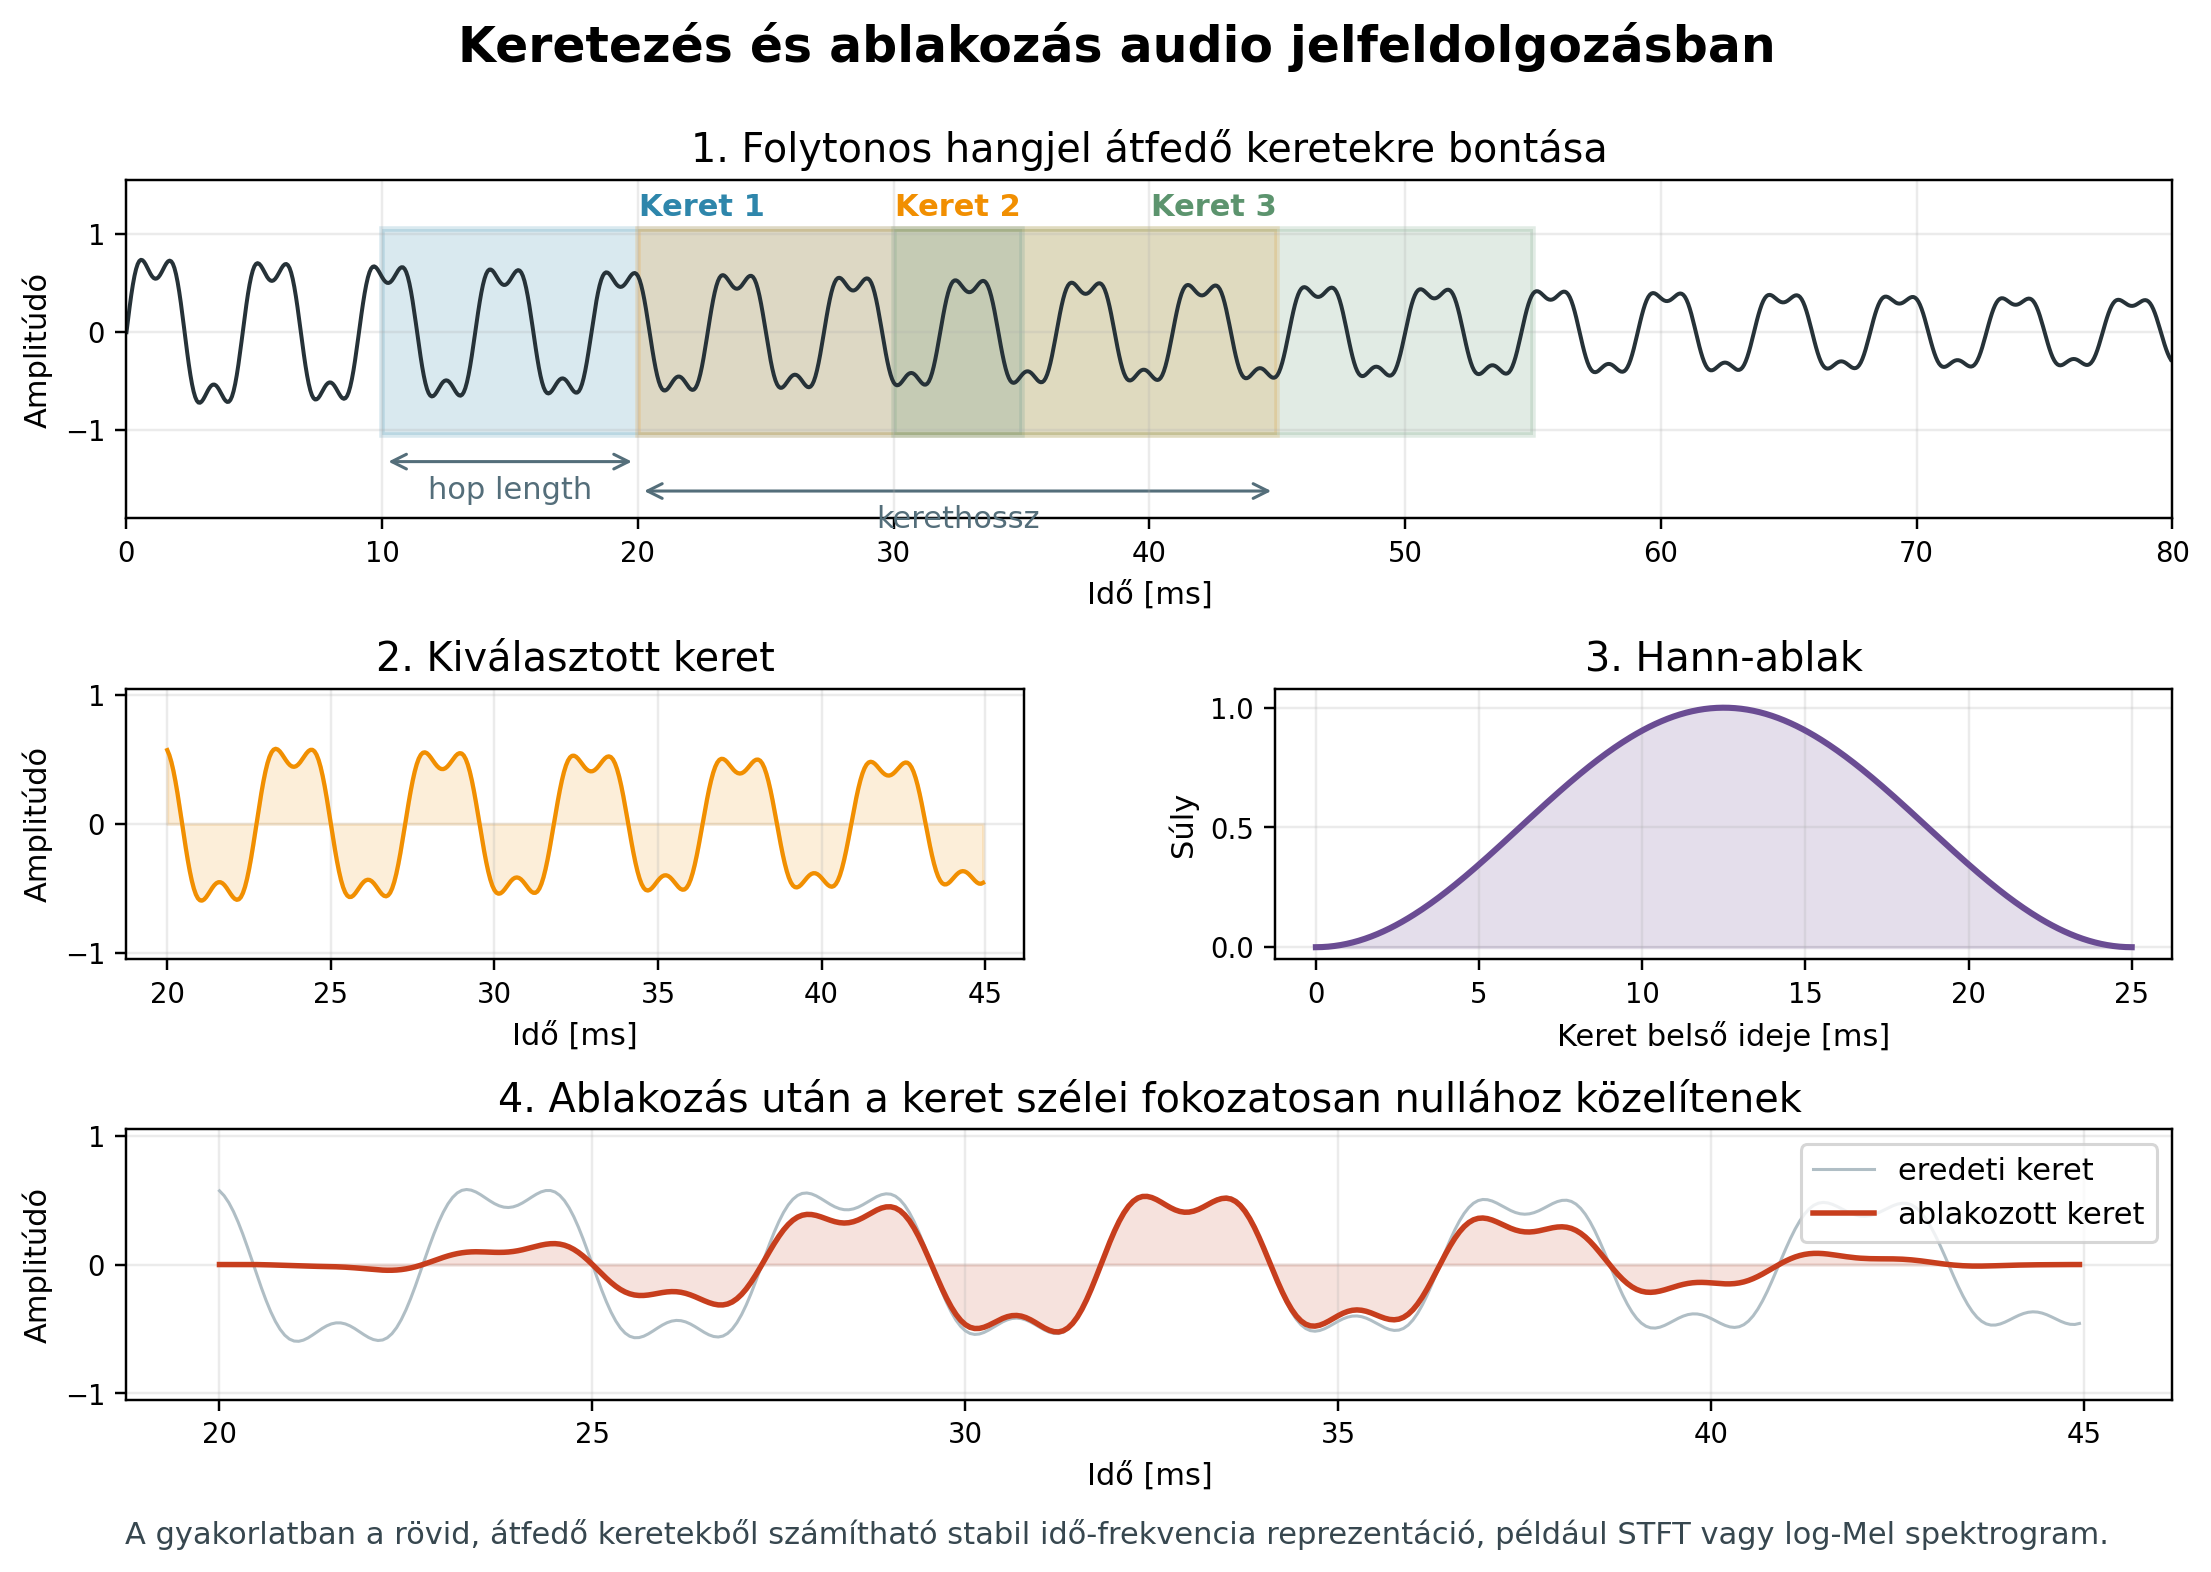
\includegraphics[width=0.82\textwidth]{fig_framing_windowing.png}
    \caption{A keretezés és ablakozás folyamata: a hangjelet rövid, átfedő ablakokra bontjuk, majd az egyes keretek széleit simítjuk.}
    \label{fig:framing_windowing}
\end{figure}

\section{Spektrogramok és tanulható bemenetek}
\label{sec:spektrogramok}

A nyers hullámforma közvetlenül is tartalmaz minden információt, de egy kis méretű saját modell számára nehezen tanulható bemenet. Ezért a hangot célszerű idő-frekvencia reprezentációvá alakítani. A rövid idejű Fourier-transzformáció (STFT) minden keretet frekvenciakomponensekre bont, az eredmény pedig egy spektrogram: egy képszerű mátrix, ahol az egyik tengely az időt, a másik a frekvenciát, a színintenzitás pedig az energiát jelöli.

\begin{figure}[H]
    \centering
    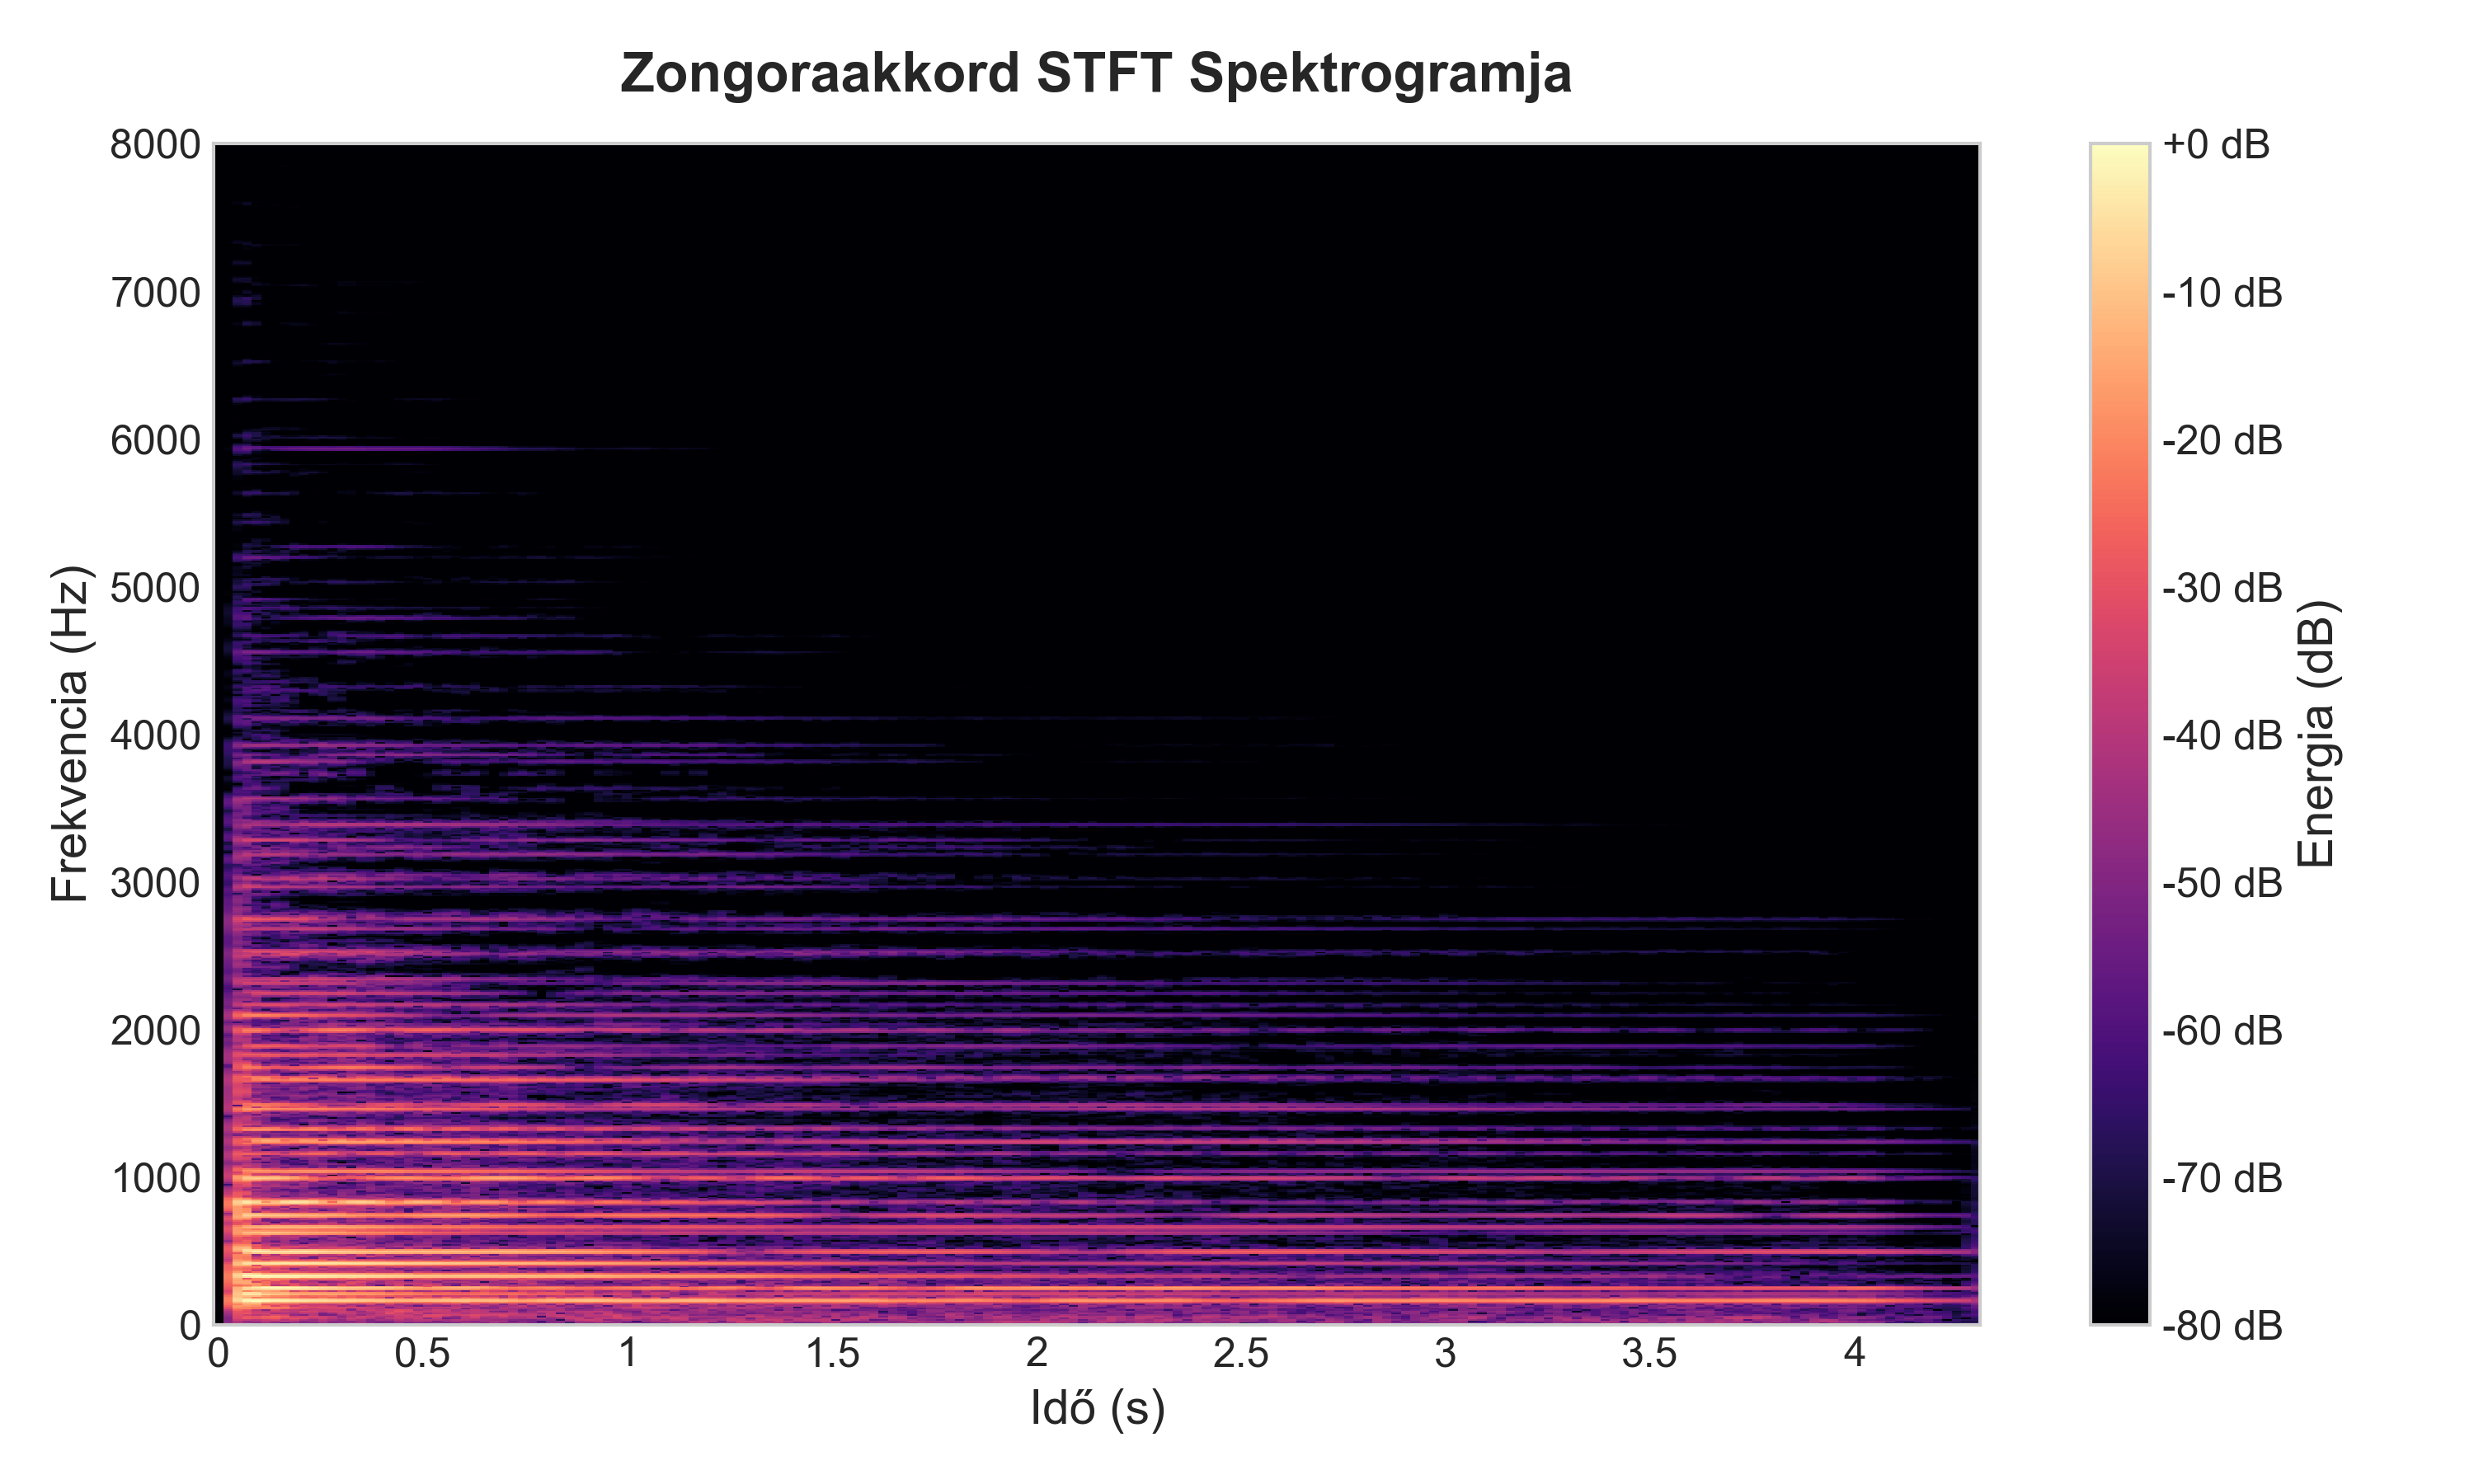
\includegraphics[width=0.78\textwidth]{fig_spectrogram_example.png}
    \caption{Egy rövid gitárhang hullámformája és STFT-spektrogramja. A spektrogramon az idő és frekvencia mentén láthatóvá válik, hol található a hang energiája.}
    \label{fig:spectrogram_example}
\end{figure}

A lineáris frekvenciaskála mellett gyakran használunk perceptuális skálákat is. Az emberi hallás az alacsony frekvenciák közötti különbségekre érzékenyebb, míg magas frekvenciákon kevésbé finom a megkülönböztetés. Ezt követi a Mel-skála: a mély tartományt részletesebben, a magas tartományt tömörebben ábrázolja. Ha az STFT után Mel-szűrőbankot és logaritmikus decibel skálázást alkalmazunk, log-Mel spektrogramot kapunk. A log-Mel bemenet zenei audiofeladatokban is gyakori, mert a CNN a spektrális és időbeli mintázatokat képszerű reprezentáción tanulhatja meg \cite{pons2018end}.

\begin{figure}[H]
    \centering
    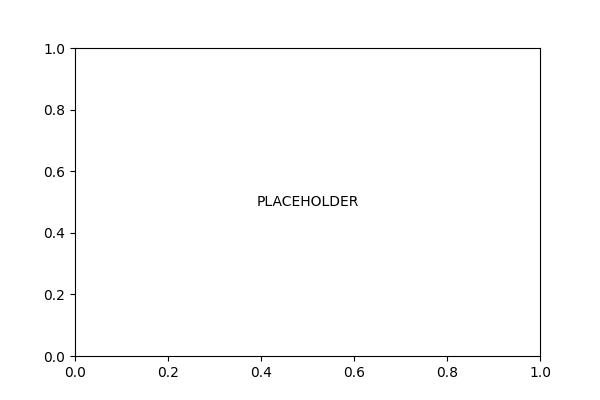
\includegraphics[width=0.82\textwidth]{fig_mel_vs_linear.png}
    \caption{Elméleti szemléltetés ugyanazon gitárhang lineáris STFT- és log-Mel spektrogramjával. A Mel-skála az emberi hallás frekvenciaérzékeléséhez igazítja a reprezentációt, ezért a mélyebb tartományt részletesebben kezeli.}
    \label{fig:mel_vs_linear}
\end{figure}

A dolgozatban három jellemzőkinyerési irányt használok összehasonlítási alapként. Az \textbf{STFT} közvetlen, lineáris frekvenciatengelyű spektrogramot ad, ezért alapvető frekvencia-idő baseline. Az \textbf{MFCC} klasszikus, tömörített audiojellemző, amely a Mel-spektrum diszkrét koszinusz transzformációjával keletkezik, és főleg hagyományos gépi tanulási feladatokban terjedt el. A \textbf{log-Mel spektrogram} a kettő között helyezkedik el: képszerű struktúrát őriz meg, de a frekvenciatengelyt az emberi halláshoz igazítja.

\begin{table}[H]
\centering
\caption{A három vizsgált bemeneti reprezentáció elméleti szerepe}
\label{tab:mfcc_vs_mel}
\begin{tabular}{p{2.6cm}p{4.0cm}p{6.4cm}}
\toprule
\textbf{Reprezentáció} & \textbf{Jelleg} & \textbf{Miért került be a dolgozatba?} \\
\midrule
STFT & Lineáris spektrogram & Megmutatja, hogyan teljesít a közvetlen frekvencia-idő ábrázolás. \\
MFCC & Tömörített kepsztrális jellemző & Klasszikus audio baseline, kisebb dimenzióval és erősebb előfeldolgozással. \\
Log-Mel & Perceptuális spektrogram & CNN-hez jól illeszkedő, képszerű és hallásközeli reprezentáció. \\
\bottomrule
\end{tabular}
\end{table}

\section{Neurális osztályozás spektrogramokon}
\label{sec:neuralis_osztalyozas}

A hangszerfelismerés felügyelt osztályozási feladat: minden tanítómintához tartozik egy bemenet és egy címke. A modell feladata, hogy a bemenet alapján hét kategória közül válasszon. Többosztályos neurális hálózatnál a kimeneti réteg tipikusan softmax aktivációt használ, amely minden osztályhoz egy valószínűségszerű értéket rendel. A prediktált osztály az lesz, amelynek a kimeneti értéke a legnagyobb.

A tanítás során a hálózat a hibás predikciók alapján módosítja a súlyait. A validációs halmaz szerepe az, hogy mérje: a modell nemcsak a tanítóadatokat jegyezte-e meg, hanem új mintákon is képes-e általánosítani. A túlilleszkedés (overfitting) akkor jelenik meg, amikor a modell a tanítóhalmazon jól teljesít, de a validációs vagy teszthalmazon gyengébben. Ennek mérséklésére használhatók például dropout rétegek, adataugmentáció, címkesimítás, valamint korai leállítás. Spektrogram-bemeneteknél az idő- és frekvenciamaszkok használata a SpecAugment módszerrel vált ismertté \cite{park2019specaugment}; a saját rendszerben ennek egyszerűsített gondolata jelenik meg tanítás közbeni maszkolásként.

Spektrogramok esetében a 2D konvolúciós neurális hálózat természetes választás, mert a bemenet képszerű: az egyik tengely az időt, a másik a frekvenciát jelöli. A konvolúciós szűrők lokális idő-frekvencia mintázatokat tanulnak, például hirtelen tranzienseket, kitartott harmonikus sávokat vagy zajos spektrális tartományokat.

Nem állítom, hogy a 2D CNN minden alternatívánál általánosan jobb. Egy SVM vagy más klasszikus modell használható lehet kézzel aggregált jellemzővektorokon, egy MLP viszont a spektrogram kilapításával elveszítené a lokális szerkezetet. Az 1D CNN inkább nyers hullámformán vagy időbeli jellemzősorozaton természetes, a CRNN pedig erősebb időbeli modellezést adhat, de összetettebb és több magyarázati terhet jelent. A saját rendszerben a 2D CNN ezért arányos kompromisszum: illeszkedik a log-Mel bemenethez, kezelhető méretű, és valós időben is futtatható.

\section{Hangszercsaládok akusztikai szemléltetése}
\label{subsec:hangszercsaladok}

A rendszer nem egyedi hangszereket, hanem hangszercsaládokat különít el. Ez a döntés akusztikailag is indokolható: az egy családba tartozó hangszerek azonos vagy hasonló hangkeltési elvük miatt rokon időbeli és spektrális mintázatokat mutathatnak. A kis adathalmaz és a valós idejű cél miatt ez a csoportosítás védhetőbb, mint sok különálló hangszerosztály kezelése.

\begin{table}[H]
\centering
\caption{A rendszerben használt hangszercsaládok és jellegzetes hullámformáik}
\label{tab:instrument_families}
\begingroup
\footnotesize
\setlength{\tabcolsep}{3pt}
\renewcommand{\arraystretch}{1.02}
\newcommand{\waveformcell}[1]{\includegraphics[width=\linewidth,height=0.72cm,keepaspectratio]{#1}}
\begin{tabular}{@{}>{\raggedright\arraybackslash}p{1.55cm}
                >{\raggedright\arraybackslash}p{2.15cm}
                >{\raggedright\arraybackslash}p{2.35cm}
                >{\raggedright\arraybackslash}p{4.35cm}
                >{\centering\arraybackslash}p{2.20cm}@{}}
\toprule
\textbf{Osztály} & \textbf{Példák} & \textbf{Hangkeltés} & \textbf{Jelleg} & \textbf{Hullámforma} \\
\midrule
Gitár & Akusztikus, elektromos gitár & Húr pengetése & Gyors attack, majd lecsengő rezgés. & \waveformcell{fig_table_guitar.png} \\
\midrule
Zongora & Zongora, e-piano & Kalapács által leütött húr & Impulzusszerű kezdet, hosszabb lecsengés. & \waveformcell{fig_table_piano.png} \\
\midrule
Vokál & Énekhang, torokének & Hangszálak rezgése & Kváziperiodikus jel, formánsokkal. & \waveformcell{fig_table_vocal.png} \\
\midrule
Vonós & Hegedű, brácsa, cselló, nagybőgő & Vonó és húr súrlódása & Kitartott, folytonos gerjesztés. & \waveformcell{fig_table_string.png} \\
\midrule
Nádfúvós & Klarinét, szaxofon, oboa, fagott & Nád rezgése & Kitartott, periodikus, rezonáns jel. & \waveformcell{fig_table_reed.png} \\
\midrule
Rézfúvós & Trombita, harsona, kürt, tuba & Ajkak rezgése fúvókán & Erős harmonikus szerkezet, nagy energia. & \waveformcell{fig_table_brass.png} \\
\midrule
Zaj/Csend & Környezeti zajok & Véletlenszerű rezgések & Aperiodikus, rendszertelen jel. & \waveformcell{fig_table_noise.png} \\
\bottomrule
\end{tabular}
\endgroup
\end{table}

A táblázatban hosszabb hullámforma-részletek szerepelnek, mert ezeken jól látszik a hang felfutása és lecsengése. Emellett kontrollált, közeli referenciahangokból külön nagyított példákat is készítettem. A legtöbb hangszer esetében A4 hangot használtam, a nagybőgő és a tuba esetében A3-at, mert ezeknél ez természetesebb regiszter. Ezek az ábrák nem tanítóadatok, hanem szemléltető példák: a periódus belső alakjára és a családon belüli hasonlóságokra nagyítanak rá.

\begin{figure}[H]
\centering
\begin{minipage}{0.48\textwidth}
    \centering
    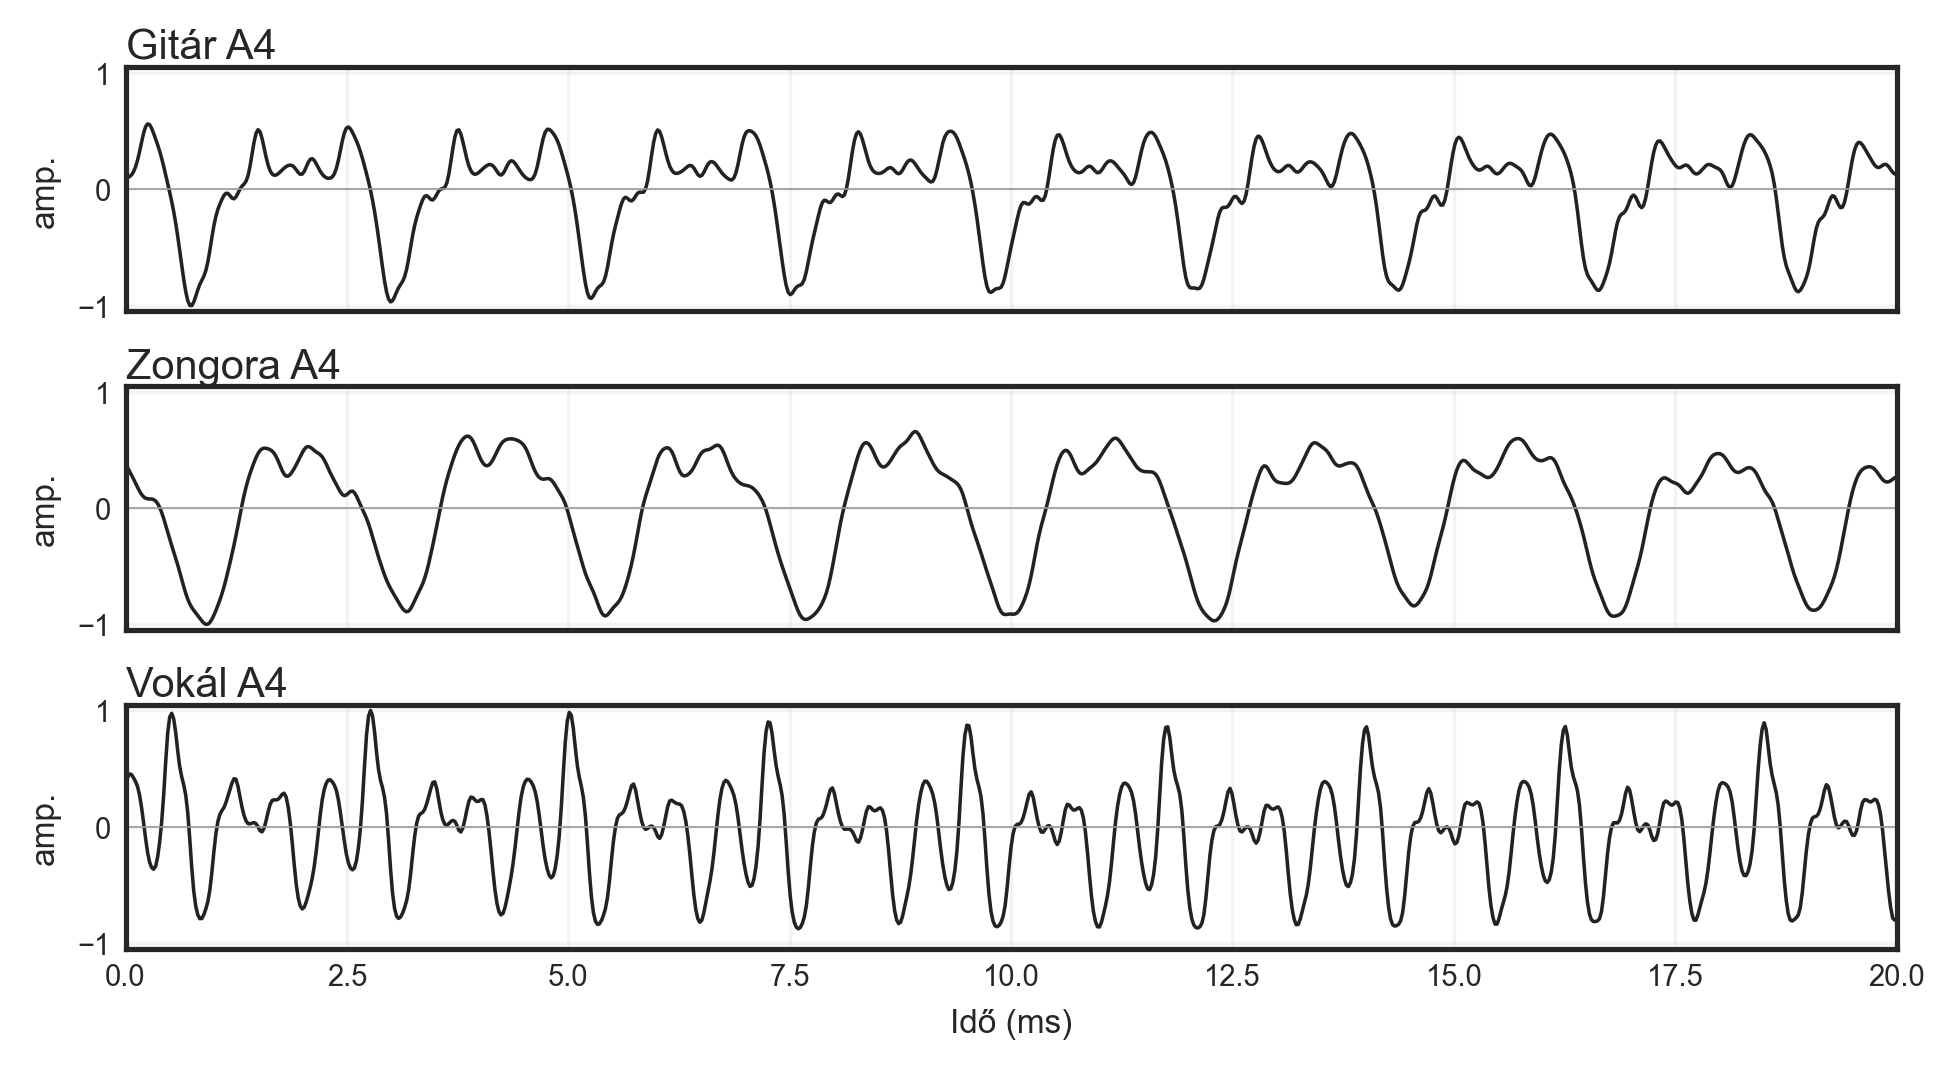
\includegraphics[width=\linewidth]{fig_asd_waveforms_solo.png}
    \footnotesize (a) Gitár, zongora és vokál
\end{minipage}\hfill
\begin{minipage}{0.48\textwidth}
    \centering
    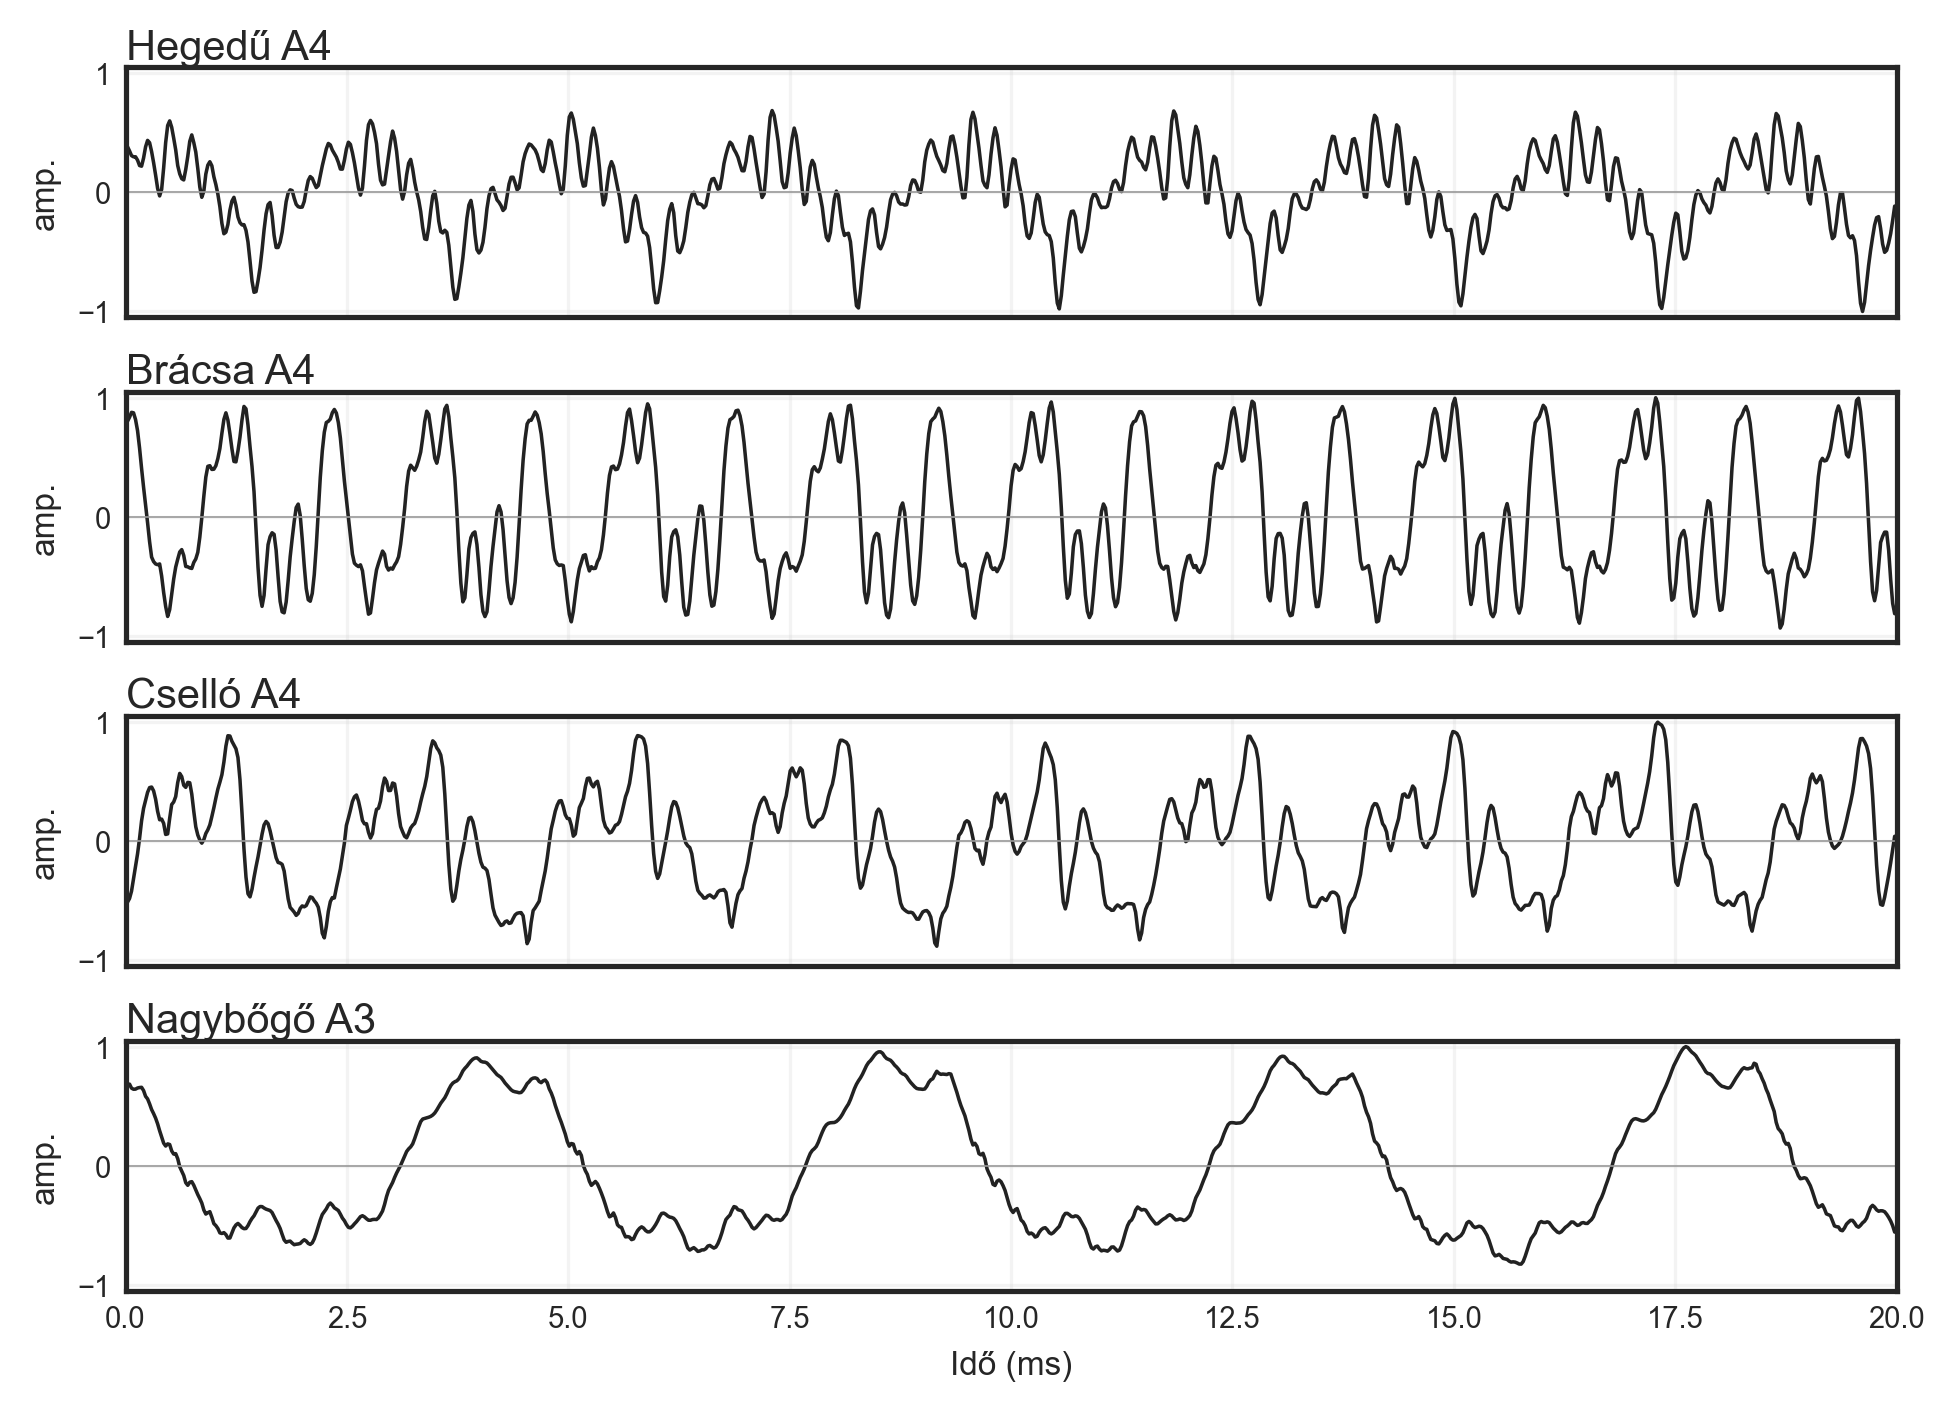
\includegraphics[width=\linewidth]{fig_asd_waveforms_string.png}
    \footnotesize (b) Vonós hangszerek
\end{minipage}

\vspace{0.4cm}

\begin{minipage}{0.48\textwidth}
    \centering
    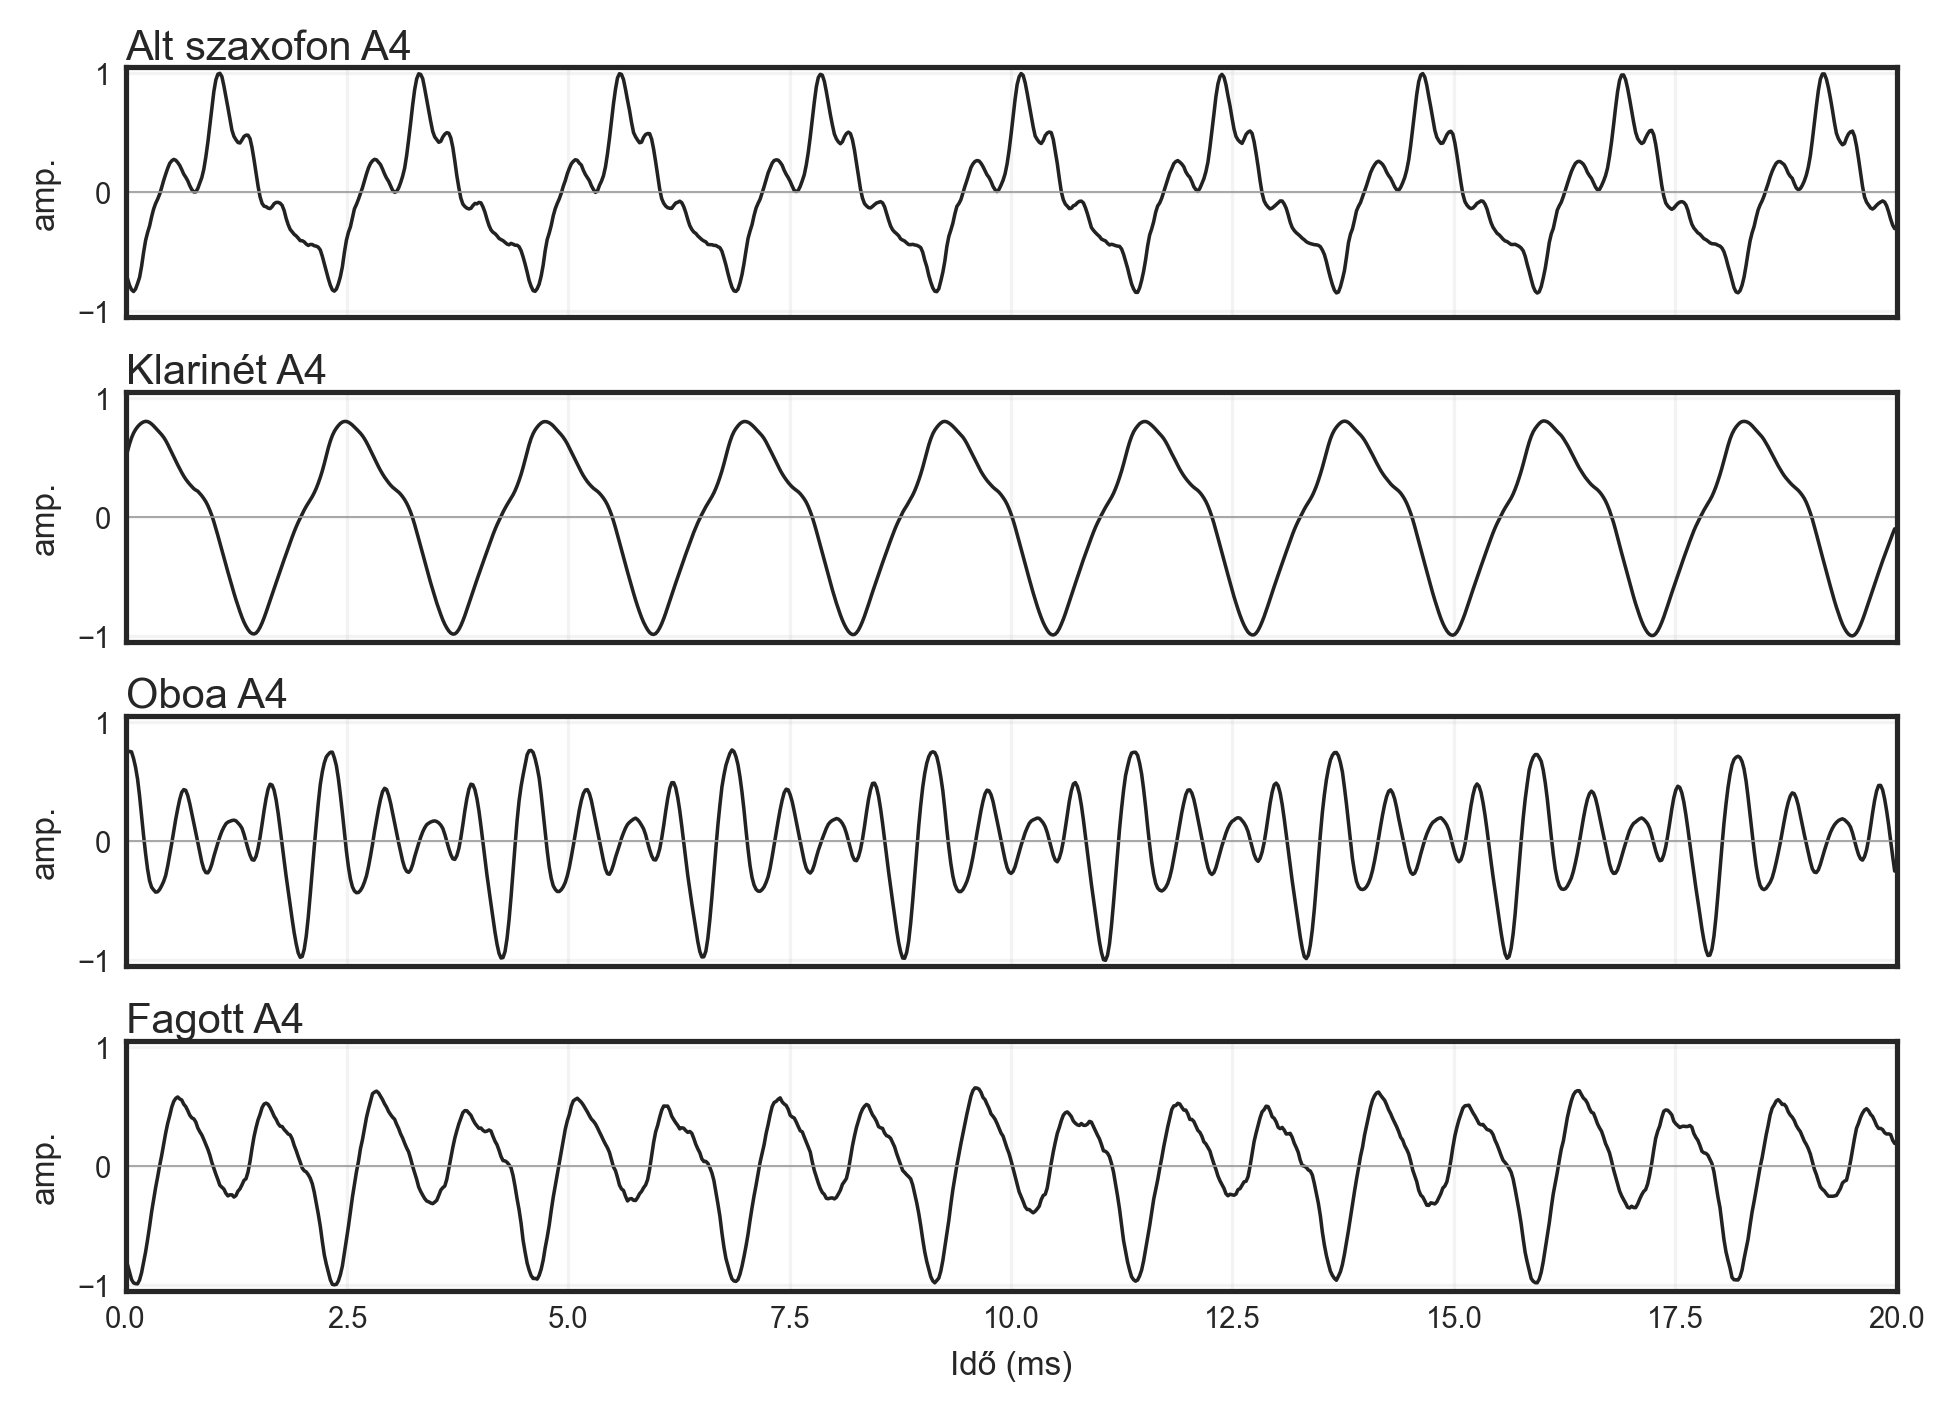
\includegraphics[width=\linewidth]{fig_asd_waveforms_reed.png}
    \footnotesize (c) Nádfúvós hangszerek
\end{minipage}\hfill
\begin{minipage}{0.48\textwidth}
    \centering
    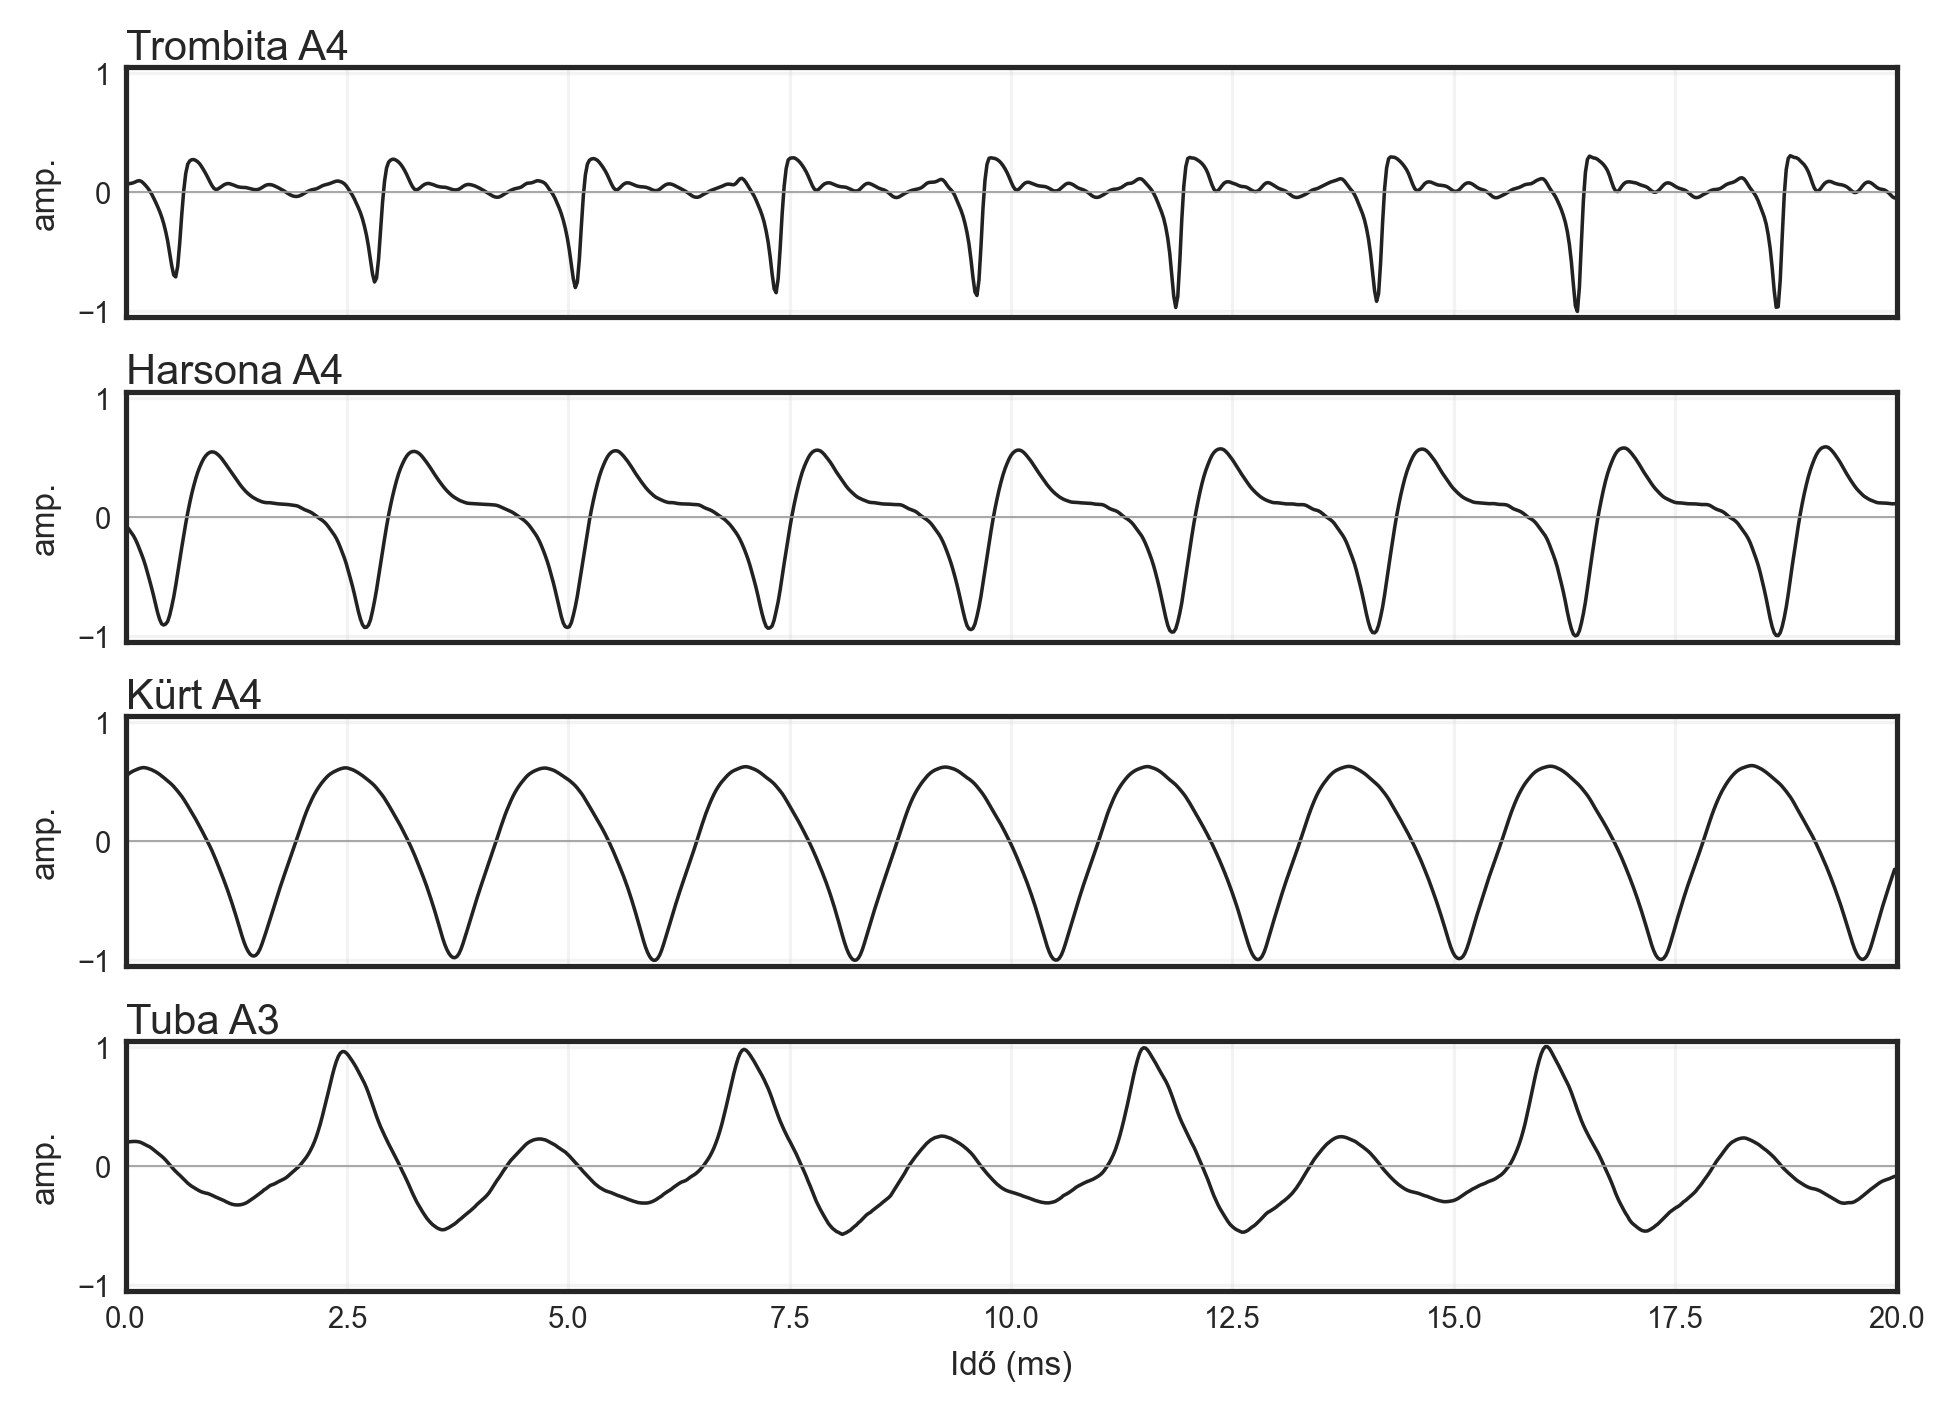
\includegraphics[width=\linewidth]{fig_asd_waveforms_brass.png}
    \footnotesize (d) Rézfúvós hangszerek
\end{minipage}
\caption{Kontrollált A4/A3 referenciahangok 20 ms-os nagyított hullámforma-részletei. A cél nem a hangerő, hanem a periodicitás és a jelalak családonkénti szemléltetése.}
\label{fig:asd_waveforms_summary}
\end{figure}

\section{Validációs kockázatok: leakage, domain shift, domain adaptation}
\label{sec:adatszivargas_elmelet}

Gépi tanulási rendszereknél a kiértékelés egyik legfontosabb kockázata az adatszivárgás, vagyis amikor a modell a tanítás során olyan információhoz jut, amely a valós használat során nem lenne elérhető. Audio esetén ez különösen könnyen előfordulhat, mert egy hosszabb felvétel egymáshoz közeli szeletei nagyon hasonlóak lehetnek. Ha ezek egyszerre kerülnek train és test halmazba, a modell túl optimista eredményt adhat.

A dolgozat szempontjából három leakage-típust érdemes kiemelni. A \textbf{train-test kontamináció} akkor jelenik meg, ha nagyon hasonló vagy azonos minták kerülnek különböző splitbe. Az \textbf{előfeldolgozási leakage} akkor fordul elő, ha például normalizálási paramétereket a teljes adathalmazból számolunk, majd azokat a tesztadatokra is alkalmazzuk. Az \textbf{augmentációs leakage} pedig akkor veszélyes, ha egy eredeti minta az egyik, annak torzított változata pedig egy másik halmazba kerül.

A valós idejű mikrofonos felismerésnél emellett megjelenik a \textbf{domain shift} is. Ez azt jelenti, hogy a tanítási környezet és a célkörnyezet eloszlása eltér: a tiszta internetes vagy stúdiószerű hangok másképp viselkednek, mint a telefonról visszajátszott és laptopmikrofonnal rögzített minták. A \textbf{domain adaptation} ennek kezelésére szolgál: a célkörnyezetből származó mikrofonos train minták bevonásával a modell jobban alkalmazkodhat ahhoz az akusztikai helyzethez, amelyben később működnie kell.

Ezek miatt a későbbi kísérletekben a train, validation és test halmazokat külön szerepben kezelem. A validáció a modellválasztásra szolgál, a test halmaz pedig csak a kiválasztott végső modellek utolsó ellenőrzésére. Így a mérési eredmények nem rekordpontosságként, hanem kontrollált, módszertanilag védhető összehasonlításként értelmezhetők.


\chapter{A rendszer specifikációi és architektúrája}
\label{chap:specifikacio}

A szakdolgozat előző fejezetében bemutatott akusztikai és mélytanulási elméleti alapokra építkezve jelen fejezet a megvalósított hangszerfelismerő rendszer mérnöki és szoftverfejlesztési tervezését ismerteti. Egy gépi tanulási alapú valós idejű hangfelismerő rendszer fejlesztése során nem csupán a neurális hálózat architektúrájára kell fókuszálni, hanem egy olyan robusztus csővezeték (pipeline) kialakítására is, amely képes a nyers adatok betöltésétől kezdve az adatok transzformációján át egészen a végfelhasználói valós idejű interakcióig minden lépést zökkenőmentesen kiszolgálni.

Ez a fejezet definiálja a rendszerrel szemben támasztott funkcionális és nem funkcionális követelményeket, bemutatja a felhasználói eseteket (Use Case), valamint részletezi az alkalmazás belső szoftverarchitektúráját és a technológiai választások hátterét.

\section{Célkitűzések és követelményelemzés}

A fejlesztés fő célkitűzése egy olyan keretrendszer létrehozása volt, amely képes előre felvett zenei adathalmazokon különböző jellemzőkinyerési módszereket alkalmazni, azokkal modern konvolúciós neurális hálózatokat tanítani, majd a legpontosabb modellt egy valós idejű (mikrofonos) környezetben is megbízhatóan futtatni.

\subsection{Funkcionális követelmények}
A funkcionális követelmények azokat a konkrét folyamatokat és szolgáltatásokat írják le, amelyeket a rendszernek feltétlenül nyújtania kell a sikeres működés érdekében:
\begin{itemize}
    \item \textbf{Adathalmazok fúziója és tisztítása:} A szoftvernek képesnek kell lennie nyílt forrású (pl. NSynth, Good-sounds) és saját gyűjtésű adathalmazok egyesítésére, a hibás vagy csendes minták algoritmikus szűrésére.
    \item \textbf{Jellemzőkinyerés (Feature Extraction):} A nyers \texttt{.wav} fájlokból automatikusan generálni kell a spektrogramokat (STFT és Mel-spektrogram) a megadott ablakozási paraméterekkel, és azokat hatékony Numpy mátrix formátumban menteni.
    \item \textbf{Modell tanítása (Training Pipeline):} Egy konfigurálható csővezeték megléte, amely betölti az előkészített adatokat, definiálja a 2D CNN architektúrát, majd korai leállás (early stopping) használatával optimalizálja a modellt, és kimenti a legjobb súlyokat.
    \item \textbf{Valós idejű predikció:} Egy önálló futtatható modul, amely másodpercenként rögzíti a számítógép mikrofonjának jelét, valós időben jellemzőt von ki, és a betanított Keras modellen lefuttatva terminálos felületen jelzi a felismert hangszercsaládot.
\end{itemize}

\subsection{Nem funkcionális követelmények}
A nem funkcionális követelmények a rendszer működésének minőségi mutatóira fókuszálnak:
\begin{itemize}
    \item \textbf{Alacsony késleltetés (Low Latency):} A valós idejű működés kritikus feltétele, hogy az 1 másodperces audio ablak rögzítése és a predikció megjelenítése között eltelt idő ne haladja meg a 200--300 milliszekundumot, ezáltal a felhasználó azonnali visszajelzést kapjon.
    \item \textbf{Erőforrás-hatékonyság:} A jellemzőkinyerésnek és a predikciónak CPU-n is zökkenőmentesen kell futnia, elkerülve a memóriaszivárgást egy végtelenített valós idejű futás (pl. folyamatos élő koncert figyelése) során.
    \item \textbf{Modularitás:} A kódnak lazán csatolt (loosely coupled) szkriptekből kell állnia, hogy a jellemzőkinyerési algoritmus, a neurális háló architektúrája vagy a mikrofonos rögzítési logika egymástól függetlenül módosítható vagy cserélhető legyen.
\end{itemize}

\section{Használati esetek (Use Case modell)}

A rendszer interakciós felületeit és főbb felhasználási forgatókönyveit egy UML Use Case diagram (\ref{fig:usecase}.~ábra) segítségével modelleztük. Két fő aktort azonosíthatunk:
\begin{enumerate}
    \item \textbf{Felhasználó / Kutató:} Az a mérnök vagy adattudós, aki a modell betanításáért és teszteléséért felelős.
    \item \textbf{Mikrofon / Bemenet (Rendszer-aktor):} A valós idejű adatáramlást biztosító hardveres periféria, amely automatikusan triggeli a rendszer predikciós eseményeit.
\end{enumerate}

\begin{figure}[htbp]
    \centering
    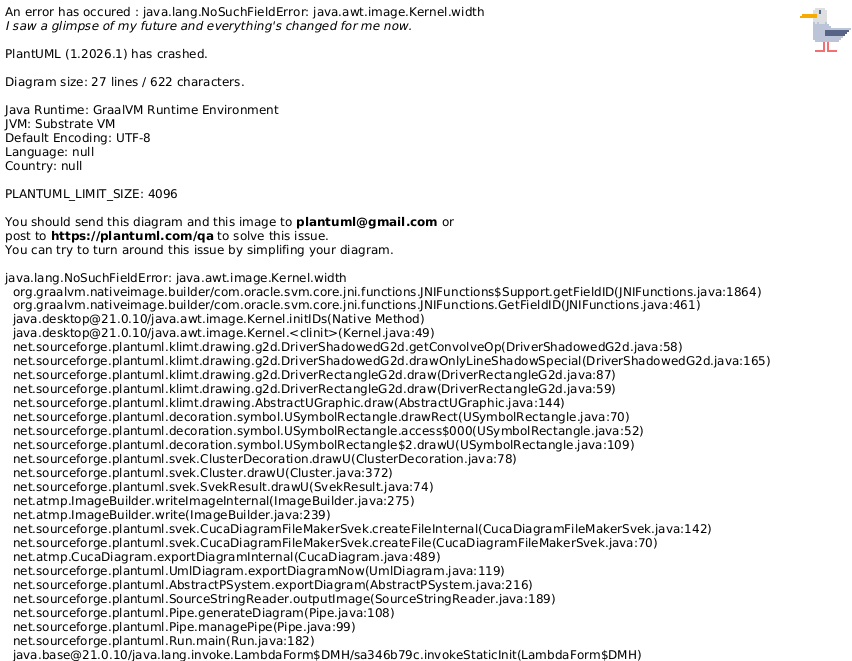
\includegraphics[width=\textwidth,height=0.5\textheight,keepaspectratio]{fig_usecase.png}
    \caption{A hangszerfelismerő rendszer főbb használati esetei (UML Use Case diagram)}
    \label{fig:usecase}
\end{figure}

A használati esetek világosan elkülönítik a "laboratóriumi" vagy kutatási fázist (adatelőkészítés és tanítás) a "produkciós" fázistól (élő predikció). Fontos tervezési szempont volt, hogy a valós idejű hangfelvétel folyamata szorosan inkluzív (\textit{<<include>>}) kapcsolatban álljon a hangszer predikciójával, hiszen a mikrofon bufferének megtelése azonnal és megszakítás nélkül aktiválja az osztályozó modult.

\section{Rendszerarchitektúra és adatfolyam}

Egy robusztus gépi tanulási rendszer architektúrája túlmutat magán a neurális hálózaton; magában foglalja az adatbeviteli (ingestion), az adatfeldolgozási (preprocessing) és az eredmény-megjelenítési (serving) rétegeket is. A megvalósított rendszer szoftverarchitektúráját és az adatok útját a \ref{fig:architecture}.~ábra UML komponensdiagramja vizualizálja.

\begin{figure}[htbp]
    \centering
    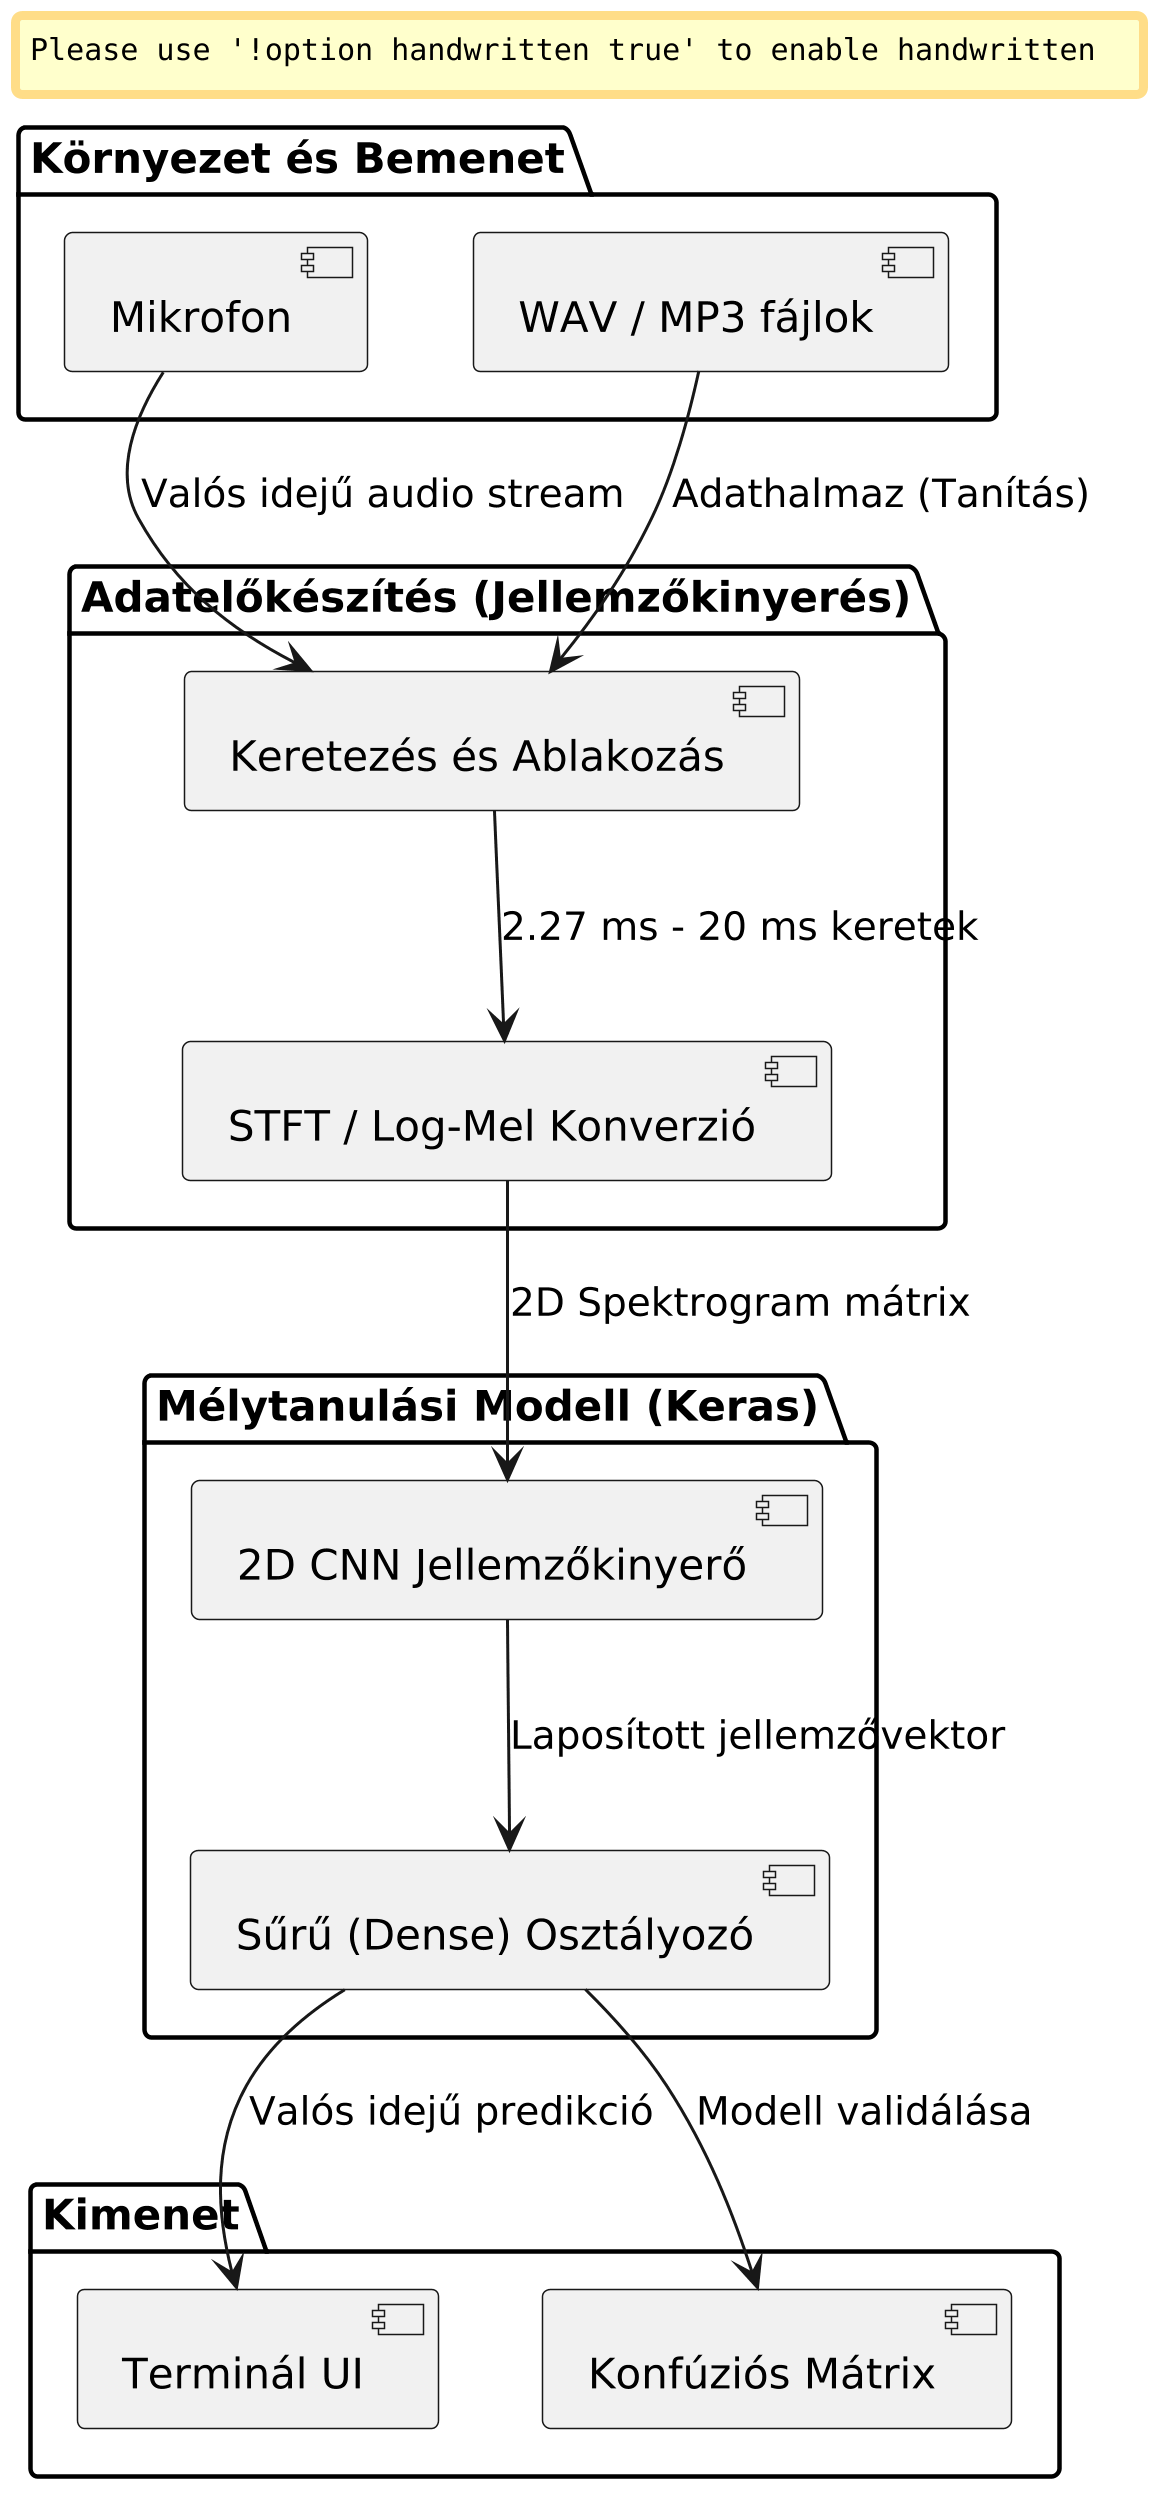
\includegraphics[width=\textwidth,height=0.65\textheight,keepaspectratio]{fig_architecture.png}
    \caption{A rendszerarchitektúra és a folyamatos adatfolyam (UML Komponensdiagram)}
    \label{fig:architecture}
\end{figure}

Az architektúra négy logikailag szeparált csomópontra (csomagra) bontható:
\begin{enumerate}
    \item \textbf{Környezet és Bemenet:} Felelős az adatok biztosításáért. Offline fázisban a \texttt{.wav} és \texttt{.mp3} fájlokból álló hatalmas adathalmazokat biztosítja lemezről, míg online fázisban a rendszer közvetlen I/O kapcsolatot tart a számítógép hangkártyájával.
    \item \textbf{Adatelőkészítés (Jellemzőkinyerés):} Ez a modul a rendszer "szíve" az akusztikai feldolgozás szempontjából. A beérkező folytonos hanghullámokat átfedő keretekre (framing) és ablakokra vágja, majd elvégzi a Fourier-transzformációt (STFT) és a Mel-szűrőbankos konverziót. Kimenete mindig egy fix dimenziójú 2D mátrix, amely már skálázva, normalizálva áll készen a modell számára.
    \item \textbf{Mélytanulási Modell (Keras):} A 2D konvolúciós rétegekből felépülő jellemzőkinyerő, majd az azt követő Sűrű (Dense) osztályozó hálózat. Bemenete a képszerű spektrogram, kimenete pedig egy valószínűségi vektor, amely a hangszer-osztályok eloszlását mutatja.
    \item \textbf{Kimenet:} A fejlesztői terminálon (CLI) megvalósított frissülő felület, amely élőben listázza a predikciós százalékokat, valamint az offline validációs fázisban itt generálódnak a konfúziós mátrixok és a tanulási görbék.
\end{enumerate}

\section{Alkalmazott technológiák és fejlesztői környezet}

A projekt megvalósítása során kiemelt szempont volt a nyílt forráskódú, ipari szabványnak számító eszközök használata, amelyek kiterjedt dokumentációval és tudományos elfogadottsággal rendelkeznek. A fejlesztés Mac OS és Windows operációs rendszereken egyaránt tesztelve lett, biztosítva a platformfüggetlenséget.

\subsection{Programozási nyelv és alapkörnyezet}
A rendszer gerincét a \textbf{Python} programozási nyelv adja. A Python választását annak egyedülálló adattudományi és gépi tanulási ökoszisztémája, valamint a gyors prototipizálást támogató absztrakciói indokolták. A numerikus számításokat, a mátrix-műveleteket és a spektrogramok memóriahatékony tárolását a \textbf{NumPy} könyvtár biztosítja, míg az adatok struktúrált elemzését és tisztítását a \textbf{Pandas} adatkeretek (DataFrames) végzik. A valós idejű, alacsony késleltetésű mikrofonos rögzítést a \textbf{sounddevice} C-alapú Python wrapper hívásai teszik lehetővé.

\subsection{Akusztikai jelfeldolgozás: Librosa}
A hangjelek beolvasásához, csendek levágásához, és a komplex idő-frekvencia transzformációk (STFT, Mel-spektrogram, MFCC) elvégzéséhez a \textbf{Librosa} könyvtárt alkalmaztam. A Librosa a zenei és audio elemzés (MIR) legelismertebb Python eszköze, amely natívan támogatja a pszichoakusztikai skálákat (például a Mel-skálát), így drasztikusan lerövidíti az akusztikai algoritmusok implementációs idejét, garantálva a laboratóriumi pontosságot.

\subsection{Mélytanulási keretrendszer: TensorFlow és Keras}
A mesterséges neurális hálózat architektúrájának definícióját, a modell tanítását és a valós idejű predikciók inferenciáját a \textbf{TensorFlow} platformon futó \textbf{Keras} API végzi. 
A Keras választása a rendkívül gyors fejlesztési ciklus, a kényelmes réteg-absztrakciók (Conv2D, MaxPooling, Dropout) és a könnyű menthetőség miatt történt. A modell betanítása és az adathalmaz validálása nagy kapacitású hardveres környezetben futott, de az inferencia (az élő felismerés) során az elkészült hálózat olyan mértékben optimalizált maradt, hogy egy átlagos számítógép processzorán (CPU) is akadás nélkül, töredékmásodperces válaszidővel képes működni.


\chapter{Részletes tervezés}
\label{chap:tervezes}A következő fejezetben részletes betekintés nyújtok, organikus adathalmazzal rendelkező, saját célú hangszerfelismerő rendszer felépítésébe, ismertetve minden tervezési lépést. Ez többek között tartalmazza az adatkészlet létrehozását, a jellemzési paramétereket, az adatbővítési beállításokat és a 2D konvolúciós neurális hálózatokat, a YAMNet transzfer tanulási architektúrát, végül a valós idejű hangszerfelismerő modul tervezését.

%% ═══════════════════════════════════════════════════════════════════════════
\section{Az adathalmaz tervezése}
\label{sec:dataset_design}

Az adathalmaz szigorú szempontrendszer szerint került összeállításra, különös figyelmet szentelve a változatos és felismerhető hangszerjátékra.

Az osztályrendszert hét osztályra osztottuk, amelyek a könnyű és klasszikus zenében előforduló leggyakoribb hangszertípusokat fogják reprezentálni. Van egy extra, környezeti zaj osztály is, amely segítségével kezeljük a csendet és a váratlan hangzavart. A 7 osztály a következő:

\begin{enumerate}
  \item[(1)] Gitár: tartalmazza az akusztikus és a kevésbé torzított elektromos gitárokat is
  \item[(2)] Zongora: tartalmazza a klasszikus és digitális zongorák egyes típusait
  \item[(3)] Vokál: tartalmaz emberi éneklést, rapet és egyéb sajátos hangképzéseket (mongol torokének, szájdob)
  \item[(4)] Húr: a vonós négyes hangszerei: hegedű, brácsa, cselló, bőgő
  \item[(5)] Nádfúvósok: mind egynádas (klarinét, szaxofon), mind kétnádas (fagott, oboa)
  \item[(6)] Rézfúvósok: legelterjedtebb változatok: trombita, harsona, kürt, tuba
  \item[(7)] Zaj: Háttér- és/vagy környezeti zajok (szél, eső, forgalom stb.), madárcsicsergés stb.
\end{enumerate}


\subsection{Saját készítésű organikus adathalmaz}
\label{subsec:own_dataset}

Kezdetben a létező adathalmazokat vizsgáltam, hogy megértsem, hogyan érdemes elkezdeni a tervezési folyamatot, és megfigyeljem, miben erősek külön-külön. Ennek érdekében az előkészítő szakaszban lefuttattam egy elemző szkriptet (\texttt{01\_analyze\_\allowbreak datasets.py}), amely feltárta az elérhető források struktúráját. Az elemzés eredményeit a \ref{tab:adathalmaz_osszehasonlitas}.~táblázat foglalja össze.

\begin{table}[H]
\centering
\caption{A vizsgált publikus adathalmazok összehasonlító elemzése}
\label{tab:adathalmaz_osszehasonlitas}
\begin{tabular}{p{2.2cm}p{4.0cm}p{4.0cm}p{3.6cm}}
\toprule
\textbf{Adathalmaz} & \textbf{Tartalom leírása} & \textbf{Fő erősségek} & \textbf{Korlátok / Miért nem felelt meg} \\
\midrule
\textbf{IRMAS}~\cite{bosch2012irmas} & Zenei részletek (3~s) szóló hangszeres és polifón szekciókkal & Valós zenei környezet, polifónia vizsgálata & Korlátozott számú és egyenetlen eloszlású hangszerkategóriák. \\
\addlinespace
\textbf{NSynth}~\cite{engel2017nsynth} & 300\,000+ db egyedi hangszeres hangjegy (4~s) & Hatalmas mintaállomány, egységes hanghossz és pitch & Csak izolált hangok, nincs benne valós zenei folytonosság és frazeálás. \\
\addlinespace
\textbf{Medley-solos-DB}~\cite{lostanlen2018medley} & Különböző sávokból kinyert szóló hangszeres részek (3~s) & Valós zenei előadásokból származó, tiszta szóló felvételek & Alacsony mintaszám egyes kategóriákban, szűkös osztályválaszték. \\
\addlinespace
\textbf{TinySOL}~\cite{cella2020tinysol} & Izolált zenekari hangszerek hangjai, különböző technikákkal & Kiváló stúdióakusztika, gazdag játéktechnikai annotációk & Kizárólag izolált hangjegyek, nem reprezentálja a folyamatos zenélést. \\
\addlinespace
\textbf{Good-sounds}~\cite{romani2015good} & Fúvós és vonós hangszerek egyedi hangjegyei & Különböző minőségű mikrofonok és felvételi minőségek & Nagyon szűk hangszerpaletta (pl. nincs gitár vagy énekhang). \\
\addlinespace
\textbf{ESC-50}~\cite{piczak2015esc} & 2000 db környezeti és háttérzaj minta (5~s) & 50 különböző zajkategória rendkívül széles spektruma & Nem tartalmaz zenei hangszereket, csak a zaj kategóriához alkalmas. \\
\bottomrule
\end{tabular}
\end{table}

Megállapítottam, hogy a meglévő adathalmazok teljes vagy részleges felhasználása nem felel meg az igényeimnek. Minden adathalmaz mintái eltérő hosszúságúak, más a hangszerosztályok eloszlása, rengeteg mintát tartalmaznak, és különböző céllal jöttek létre. Emiatt – bár kiváló tervezési alapul szolgáltak – a feldolgozásuk egységesítése komplex feladat lenne, és az átválogatásuk is rengeteg időt igényelne. Egy organikus, a saját elképzeléseim alapján összeállított adathalmaz biztosabb és átláthatóbb alapokat nyújt egy jól működő modell megteremtéséhez. 
Ez alól kivételt képezett az ESC-50, amely sokféle környezeti és háttérzaj-mintát foglal magába, így hiánypótlóként szolgált egy mindenre kiterjedő zajos adathalmaz összeállításához.

Az interneten található zenei felvételekből válogattam, figyelmet fordítva az aktuális hangszerek karakterességének kiemelésére és a zenei játék változatosságára. Minden hangszerosztályhoz (gitár, zongora, ének, vonós, nád- és rézfúvós) nagyjából 100--150 darab interneten elérhető felvételt választottam ki, amelyekből az eredeti forrás zenei tartalmának függvényében 5 másodperces blokkokat vágtam ki. 

Ezen a ponton egy kritikus tervezési döntést hoztam a gépi tanulásban gyakran felmerülő adatszivárgás (data leakage) elkerülése érdekében. Ha a darabolást rögtön végrehajtom, majd az összes 1 másodperces szeletet utólag osztom szét, nagy az esélye annak, hogy ugyanannak a hangszernek ugyanabból a zenei frázisából kerüljenek minták mind a tanító (train), mind a validációs (val) vagy teszt (test) halmazba. Ez túlzottan optimista, hamis eredménybecsléshez (túltanuláshoz, azaz overfittinghez) vezetne, mivel a modell szinte azonos hangokat látna a teszteléskor, mint a tanításkor.

Ennek elkerülésére a \texttt{01\_prepare\_clean\_dataset.py} szkript segítségével először a teljes, 5 másodperces blokkokat kevertem meg és osztottam fel a tanító (70\%), validációs (15\%) és tesztelő (15\%) halmazokra. Ezt a műveletet úgynevezett \textbf{rétegzett (stratified) felosztással} végeztem el, ami garantálja, hogy a szkript minden egyes hangszerosztálynál önállóan és szigorúan betartsa ezt az arányt, így az osztályok eloszlása mindhárom halmazban (train, val, test) tökéletesen megegyező és kiegyensúlyozott marad. A szkript csak ezután – a már szigorúan szeparált blokkokat – szeletelte fel 1 másodperces, átfedésmentes klipekre, megőrizve a szeparáció integritását. Ezáltal biztosítható, hogy a kiértékelési halmazok (val/test) eredményei teljesen megbízhatóak, és a modell nem tud ,,csalni''.

Ez a folyamat hangszertípusonként nagyjából 500 darab, többnyire monofón, stúdió- és szobaminőségű mintát eredményezett. A teljes tiszta adathalmaz (beleértve az ESC-50-ből származó kiterjedt zaj osztályt is) így összesen 4428 mintából áll.

Fontosnak tartom hangsúlyozni, hogy az internetről gyűjtött zenei hangmintákat kizárólag kutatási és oktatási (akadémiai) célokra használom fel. Ezeket a mintákat önmagukban nem teszem közzé, nem terjesztem nyilvánosan, és semmilyen kereskedelmi vagy pénzszerzési célra sem használom fel. Ez a megközelítés teljesen analóg a nagy technológiai vállalatok által alkalmazott gyakorlattal, ahol a nyilvánosan elérhető adatokat szigorúan a modellek tanítására használják fel (a szabad felhasználás, azaz a \textit{fair use} elve alapján), miközben maguk a nyers forrásfájlok zártak maradnak.

Az adathalmaz eloszlását ezen lépés után a \ref{fig:organic_class_distribution}.~ábra szemlélteti.

\begin{figure}[H]
\centering
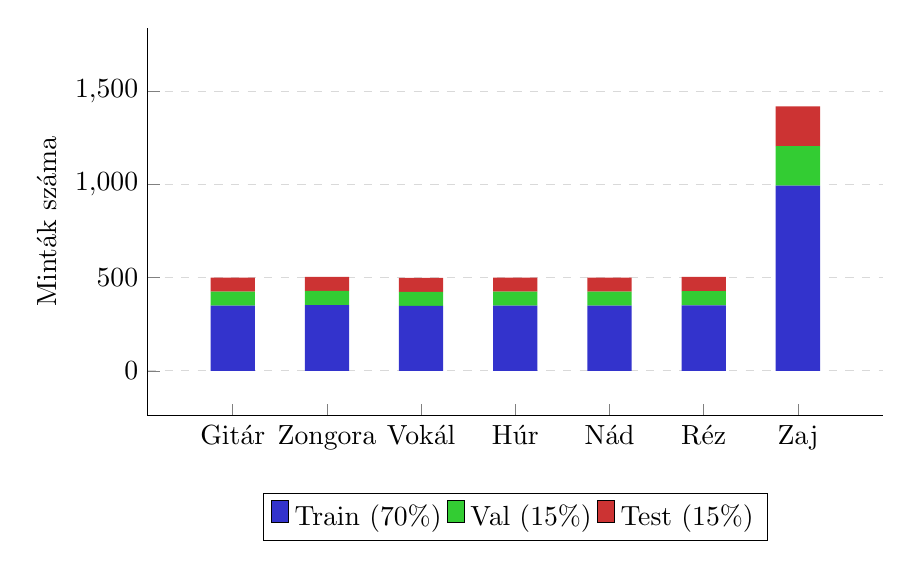
\begin{tikzpicture}
\begin{axis}[
    ybar stacked,
    bar width=16pt,
    enlargelimits=0.15,
    ylabel={Minták száma},
    symbolic x coords={Gitár, Zongora, Vokál, Húr, Nád, Réz, Zaj},
    xtick=data,
    ymin=0,
    ymax=1600,
    width=0.9\textwidth,
    height=6.5cm,
    axis x line*=bottom,
    axis y line*=left,
    ymajorgrids=true,
    grid style={dashed, gray!30},
    legend style={at={(0.5,-0.2)}, anchor=north, legend columns=-1},
]
\addplot[fill=blue!60!gray, draw=none] coordinates {
    (Gitár,350) (Zongora,353) (Vokál,349) (Húr,350) (Nád,350) (Réz,352) (Zaj,994)
};
\addplot[fill=green!60!gray, draw=none] coordinates {
    (Gitár,75) (Zongora,76) (Vokál,75) (Húr,75) (Nád,75) (Réz,76) (Zaj,213)
};
\addplot[fill=red!60!gray, draw=none] coordinates {
    (Gitár,75) (Zongora,76) (Vokál,75) (Húr,75) (Nád,75) (Réz,76) (Zaj,213)
};
\legend{Train (70\%), Val (15\%), Test (15\%)}
\end{axis}
\end{tikzpicture}
\caption{A saját gyűjtésű organikus adathalmaz eloszlása a szeparált szeletelés után}
\label{fig:organic_class_distribution}
\end{figure}

\subsection{Mikrofonos újrafelvétel a valós idejű kiértékelés felkészítésének érdekében}
\label{subsec:mic_recording}

A kezdeti adatkészleteim önmagukban kevés zajos mintát tartalmaznak, melyeket az eredeti felvételt készítő eszköz mikrofonjával rögzítettek. Minden mikrofonnak saját jellemzői vannak: frekvencia-válasza, érzékenysége, torzítása, belső zaja és maximális hangnyomásszintje (SPL). Mivel a projektem célja a valós idejű hangszerfelismerés is, a modell stabilitásának kialakításához elengedhetetlen az optimalizálás a saját eszközünkre, amellyel a predikció megtörténik.

A valós idejű kiértékelésre való felkészítés érdekében egy speciális eljárást találtam ki. Mivel nem férek hozzá, és játszani sem tudok ennyiféle hangszeren, a telefon hangszóróján játszom vissza a mintákat a laptopom beépített mikrofonjába. A feljátszás 10--30~cm távolságról történik a beépített mikrofon pontos helyzetétől mérve, hogy a hang a közelség miatt se legyen túl torz, de a távolság miatt se váljon értelmezhetetlenné vagy túl halkká.

A több ezer minta egyenkénti feljátszása helyett egy automatizált munkafolyamatot alakítottam ki. Egyetlen közös script (\texttt{02\_acquire\_\allowbreak mic\_\allowbreak data.py}) segítségével először osztályonként összefűzöm a tiszta adatok 70\%-át kitevő tanító (train) halmaz mintáit, a telefonról visszajátszva egyben felvételezem, majd a szoftver automatikusan újra felszeleteli azokat. Ezt követően egy dedikált script (\texttt{03a\_merge\_\allowbreak mic\_\allowbreak to\_\allowbreak train.py}) végzi el az új mikrofonos minták célirányos fúzióját a tanító adathalmazzal. Kritikus tervezési döntés, hogy ezt a mikrofonos újrafelvételt kizárólag a tanító halmazon végzem el, míg a validációs és teszt halmazok teljesen ,,tiszták'' maradnak. Ezzel elkerülhető az adatszivárgás (data leakage): ha a modell a tesztelés során a saját mikrofonunk már megismert alapzajával és torzításával találkozna, a specifikus zajokat felismerve ,,csalhatna''. A tiszta kiértékelő halmazok garantálják, hogy a modell valós generalizációs képességét mérjük egy számára teljesen ismeretlen akusztikai környezetben.

Ebben az esetben azonban a telefon lejátszásának és a laptop beépített mikrofonjának felvételezésének szinkronizációjára van szükség. A pontos szinkronizáció megvalósításához a következő folyamatot alakítottam ki: a \texttt{02\_acquire\_\allowbreak mic\_\allowbreak data.py} script első előkészítő lépése a hanganyag legelejére egy 1~másodperces, 440~Hz-es szinuszos szinkronizációs sípszót generál, a hangszeres mintákat pedig 0,2~másodperces csendes szakaszokkal választja el egymástól. A telefonról történő visszajátszás alatt ugyanez a script rögzíti a beérkező jelet 16\,000~Hz-es mintavételezéssel, mono formátumban. Végül a script szeletelő funkciója a Librosa könyvtár segítségével detektálja a felvétel elején található sípszó végét, majd ettől a ponttól kiindulva felszeleteli a hanganyagot pontosan 1~másodperces egységekre, miközben automatikusan kiszűri a csendes részeket.
 
Az automatizált mikrofonos újrafelvételi és szeletelési munkafolyamatot a \ref{fig:mic_recording_pipeline}.~ábra szemlélteti.

\begin{figure}[H]
\centering
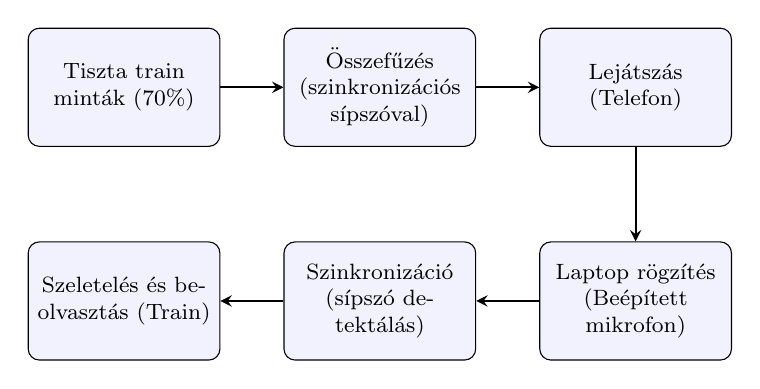
\begin{tikzpicture}[
    node distance=1.2cm and 0.8cm,
    block/.style={draw, rectangle, minimum height=1.5cm, minimum width=2.4cm, fill=blue!5!white, text width=2.2cm, align=center, font=\footnotesize, rounded corners},
    arrow/.style={thick,->,>=stealth}
]
% Nodes
\node (orig) [block] {Tiszta train minták (70\%)};
\node (concat) [block, right=0.8cm of orig] {Összefűzés (szinkronizációs sípszóval)};
\node (play) [block, right=0.8cm of concat] {Lejátszás (Telefon)};
\node (record) [block, below=1.2cm of play] {Laptop rögzítés (Beépített mikrofon)};
\node (sync) [block, left=0.8cm of record] {Szinkronizáció (sípszó detektálás)};
\node (slice) [block, left=0.8cm of sync] {Szeletelés és beolvasztás (Train)};

% Arrows
\draw [arrow] (orig) -- (concat);
\draw [arrow] (concat) -- (play);
\draw [arrow] (play) -- (record);
\draw [arrow] (record) -- (sync);
\draw [arrow] (sync) -- (slice);

\end{tikzpicture}
\caption{A mikrofonos újrafelvételi és szinkronizált szeletelési folyamat lépései}
\label{fig:mic_recording_pipeline}
\end{figure}

Az újrafelvételi folyamat eredményeképpen kizárólag a tanító (train) halmaz eredeti, tiszta mintái mellé kerülnek be az új, mikrofonos karakterisztikájú minták. Ez a bővítmény hordozza a laptopom beépített mikrofonjának torzításait, frekvencia-válaszát és belső zaját, felkészítve ezzel a modellt a valós idejű kiértékelés kihívásaira. Az adathalmaz aktuális összetételét és a minták felhalmozódását a \ref{fig:mic_recorded_distribution}.~ábra szemlélteti egymásra épülő (stacked) formában, halmazok (Train, Val, Test) és rögzítési mód (Tiszta, Mikrofonos) szerint különválasztva. Fontos megjegyezni, hogy a Zaj osztály esetében nem végeztem ilyen újrafelvételt: az ebből a kategóriából származó ESC-50 minták eleve valós környezeti és háttérzajokat tartalmaznak, így teljesen feleslegesnek tartottam a szélzaj vagy az eső hangját telefonról visszajátszva újra felvenni, ráadásul ez a lejátszási lánc miatt szükségtelen egyedi torzulásokat is vinne a tiszta zajmintákba.

\begin{figure}[H]
\centering
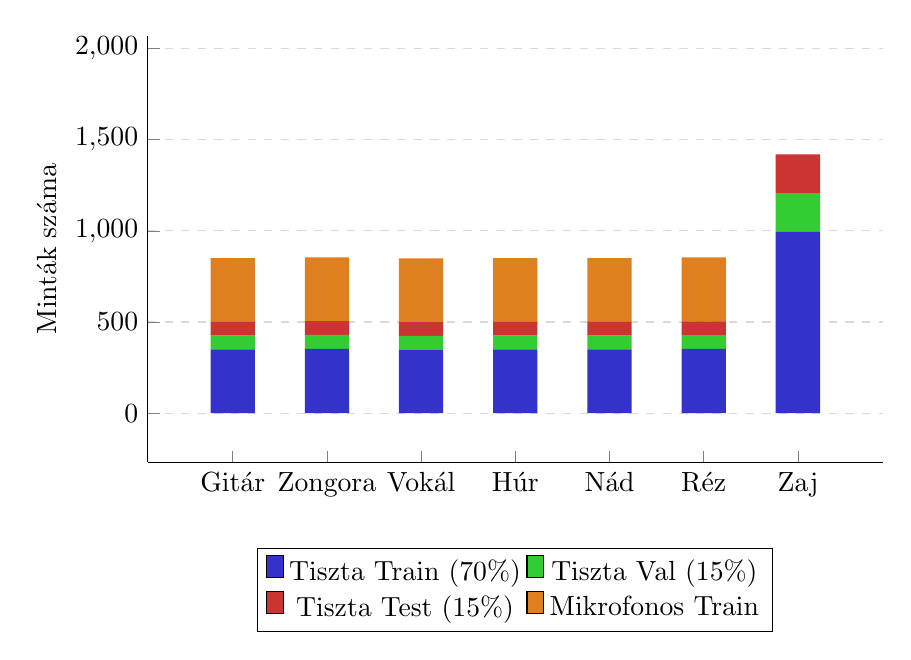
\begin{tikzpicture}
\begin{axis}[
    ybar stacked,
    bar width=16pt,
    enlargelimits=0.15,
    ylabel={Minták száma},
    symbolic x coords={Gitár, Zongora, Vokál, Húr, Nád, Réz, Zaj},
    xtick=data,
    ymin=0,
    ymax=1800,
    width=0.9\textwidth,
    height=7cm,
    axis x line*=bottom,
    axis y line*=left,
    ymajorgrids=true,
    grid style={dashed, gray!30},
    legend style={at={(0.5,-0.2)}, anchor=north, legend columns=2},
]
\addplot[fill=blue!60!gray, draw=none] coordinates {
    (Gitár,350) (Zongora,353) (Vokál,349) (Húr,350) (Nád,350) (Réz,352) (Zaj,994)
};
\addplot[fill=green!60!gray, draw=none] coordinates {
    (Gitár,75) (Zongora,76) (Vokál,75) (Húr,75) (Nád,75) (Réz,76) (Zaj,213)
};
\addplot[fill=red!60!gray, draw=none] coordinates {
    (Gitár,75) (Zongora,76) (Vokál,75) (Húr,75) (Nád,75) (Réz,76) (Zaj,213)
};
\addplot[fill=orange!75!gray, draw=none] coordinates {
    (Gitár,350) (Zongora,350) (Vokál,350) (Húr,350) (Nád,350) (Réz,350) (Zaj,0)
};
\legend{Tiszta Train (70\%), Tiszta Val (15\%), Tiszta Test (15\%), Mikrofonos Train}
\end{axis}
\end{tikzpicture}
\caption{A saját tiszta és az újrafelvételezett zajos minták megoszlása az adathalmazban}
\label{fig:mic_recorded_distribution}
\end{figure}

\subsection{Végső adathalmaz összeállítása}
\label{subsec:final_dataset}



Egy konzisztens és pontos adathalmaz nagyban segíti a neurális hálózat tanulási folyamatát. A megtervezett adatfolyam két fő könyvtárra támaszkodik: a \texttt{dataset\_clean} (amely a tiszta internetes mintákat tartalmazza, összesen 4428 darabot) és a \texttt{dataset\_mic} (amely a \texttt{train} halmaz esetében már tartalmazza az újrafelvett, mikrofonos mintákat is, így összesen 6492 darabot számol).

Amikor a jellemzőkinyerő script lefut, az adataugmentációs lépéseket (reverb, zajkeverés, torzítás) ,,on-the-fly'', azaz dinamikusan végzi el a memóriában. Ennek eredményeképpen a feldolgozott (kinyert) jellemzők száma a tanítási fázishoz kibővül: a tiszta adathalmazban 5927-re, míg a mikrofonos (augmented) adathalmazban 8335-re. Ez a megközelítés rendkívül stabil alapokat biztosít a hálózat számára.

\section{Jellemzőkinyerés tervezése}
\label{sec:feature_extraction}

A nyers audiojelek nem alkalmasak közvetlenül a konvolúciós neurális hálózat bemeneteként, mivel a hullámforma (waveform) időtartománybeli ábrázolása túl magas dimenziójú és nehezen tanulható mintázatokat tartalmaz. Emiatt szükséges egy megfelelő 2D-s spektrális jellemzőkinyerési eljárás kiválasztása. A tervezés során három elterjedt módszert vizsgáltam meg a \texttt{librosa}~\cite{mcfee2015librosa} könyvtár implementációira építve: a rövid idejű Fourier-transzformációt (STFT), a Mel-frekvenciás kepsztrális együtthatókat (MFCC), valamint a Log-Mel spektrogramot. Mindhárom jellemzőtípus azonos ablakozási paraméterekkel készül:

\begin{itemize}
  \item FFT ablakméret: $n\_fft = 1024$ minta,
  \item Ugrási hossz (hop length): $hop\_length = 512$ minta,
  \item Mintavételi frekvencia: $SR = 16\,000$ Hz.
\end{itemize}

1~másodperces audioszelet esetén ($16\,000$ minta, $hop\_length = 512$) az időtengely mérete: $\lfloor 16000 / 512 \rfloor + 1 = 32$ időkeret.

\subsection{Log-Mel spektrogram}

A Log-Mel spektrogram előállításának lépései:

\begin{enumerate}
  \item Mel-szűrőbank alkalmazása $n\_mels = 64$ sávval az STFT kimenetére,
  \item Teljesítmény-decibelre konvertálás: $S_{dB} = 10 \cdot \log_{10}(S_{mel} / S_{ref})$.
\end{enumerate}

Az eredmény egy $64 \times 32$ méretű mátrix, amelyet a CNN egycsatornás képként ($64 \times 32 \times 1$) kap meg. A Log-Mel spektrogram előnye, hogy a Mel-skála a hallórendszer nemlineáris frekvenciaérzékelését modellezi, így a hangszerek jellegzetes formánsai és felharmonikusai hatékonyan jelennek meg.

\subsection{STFT spektrogram}

Az STFT (Short-Time Fourier Transform) spektrogram az amplitúdó-spektrum decibelre konvertált változata:

$$X_{dB}(f,t) = 20 \cdot \log_{10}\left(\frac{|X(f,t)|}{X_{ref}}\right)$$

Az eredmény egy $513 \times 32$ méretű mátrix ($n\_fft/2 + 1 = 513$ frekvenciasáv). Ez a reprezentáció a teljes lineáris frekvenciaskálát megtartja.

\subsection{MFCC (Mel-Frequency Cepstral Coefficients)}

Az MFCC-t $n\_mfcc = 40$ együtthatóval számolom. Az MFCC a spektrális burkoló tömör reprezentációja; az eredmény egy $40 \times 32$ méretű mátrix. Az MFCC jellemzőkre Z-score normalizálást alkalmazok sávonként:

$$\hat{x}_i = \frac{x_i - \mu_i}{\sigma_i + \epsilon}$$

ahol $\mu_i$ és $\sigma_i$ az $i$-edik MFCC sáv átlaga és szórása, $\epsilon = 10^{-10}$.

\subsection{Nyers hanghullám (Raw waveform)}

A frekvenciatartománybeli jellemzők mellett közvetlenül kinyerjük és elmentjük a nyers, időtartománybeli audiojelet is. 1 másodperc esetén ez egy 16\,000 elemű, 1D-s tömb. Bár a hagyományos 2D CNN hálózatok számára ez az ábrázolás nem ideális, a mélyebb transzfer tanulási eljárások (például a YAMNet) pontosan ezt a nyers formátumot várják bemenetként.

\subsection{A megfelelő jellemzőkinyerési eljárás kiválasztása}
\label{subsec:feature_selection}

A három vizsgált jellemzőtípus (STFT, MFCC, Log-Mel) alapos elemzése után a következő szempontokat mérlegeltem a neurális hálózat bemenetének kiválasztásakor:
\begin{itemize}
  \item Az \textbf{STFT spektrogram} előnye, hogy a teljes lineáris frekvenciaspektrumot megőrzi, azonban a $513 \times 32$-es méret túl nagy dimenziójú bemenetet eredményezne. Ez nemcsak jelentősen növelné a hálózat paraméterszámát és a tanítási időt, de a magas frekvenciás sávok felesleges részletgazdagsága miatt a túlilleszkedés (overfitting) kockázatát is növelné.
  \item Az \textbf{MFCC} bár rendkívül kompakt ($40 \times 32$), a diszkrét koszinusz transzformáció (DCT) alkalmazásával eldobja a spektrális finomszerkezetet és a felharmonikusok közötti összefüggéseket. Ez beszédfelismerésnél előnyös (ahol a hangmagasságtól független fonémákat keressük), de a zenei hangszerek osztályozásánál a felharmonikusok aránya hordozza a hangszín lényegi információját, így az MFCC használata információvesztéssel járna.
  \item A \textbf{Log-Mel spektrogram} ($64 \times 32$) jelenti a legjobb kompromisszumot. A Mel-skála nemlineárisan sűríti a frekvenciatengelyt az emberi hallásnak megfelelően (finomabb felbontás a mély tartományban, durvább a magasban), így megőrzi a hangszerek hangszínének felismeréséhez szükséges felharmonikus-szerkezetet, miközben alacsonyan tartja a bemeneti dimenziót.
\end{itemize}

A fenti szempontok alapján a valós idejű hangszerfelismerő rendszerem elsődleges jellemzőjének a \textbf{Log-Mel spektrogramot} választottam, a konvolúciós neurális hálózat architektúráját és a valós idejű feldolgozást is erre a bemenetre terveztem. A három vizsgált jellemző legfontosabb tulajdonságait a~\ref{tab:feature_comparison_properties}. táblázat foglalja össze.

\begin{table}[H]
  \centering
  \caption{A három vizsgált jellemzőkinyerési módszer összehasonlító elemzése}
  \label{tab:feature_comparison_properties}
  \resizebox{\textwidth}{!}{%
  \begin{tabular}{lllp{4.5cm}p{4.5cm}}
    \toprule
    \textbf{Jellemző} & \textbf{Dimenzió} & \textbf{Frekvencia-skála} & \textbf{Fő előny} & \textbf{Fő hátrány} \\
    \midrule
    STFT & $513 \times 32$ & Lineáris & Megőrzi a teljes spektrális finomszerkezetet. & Túl nagy dimenziószám, növeli a túlilleszkedés kockázatát. \\
    \midrule
    Log-Mel & $64 \times 32$ & Logaritmikus Mel-skála & Az emberi hallást modellezi; megőrzi a felharmonikusokat. & Enyhe információvesztés a frekvenciatömörítés miatt. \\
    \midrule
    MFCC & $40 \times 32$ & Kepsztrális & Rendkívül kompakt és dekorrelált reprezentáció. & Diszkrét koszinusz transzformáció miatt eldobja a felharmonikusokat. \\
    \bottomrule
  \end{tabular}%
  }
\end{table}

\subsection{Normalizálás}

A kiválasztott Log-Mel jellemzőket globális min-max normalizálással skálázom a $[0, 1]$ intervallumra:

$$\hat{X} = \frac{X - X_{min}}{X_{max} - X_{min} + \epsilon}$$

Ez biztosítja, hogy a CNN bemenete konzisztens értéktartományban maradjon.

\begin{figure}[H]
  \centering
  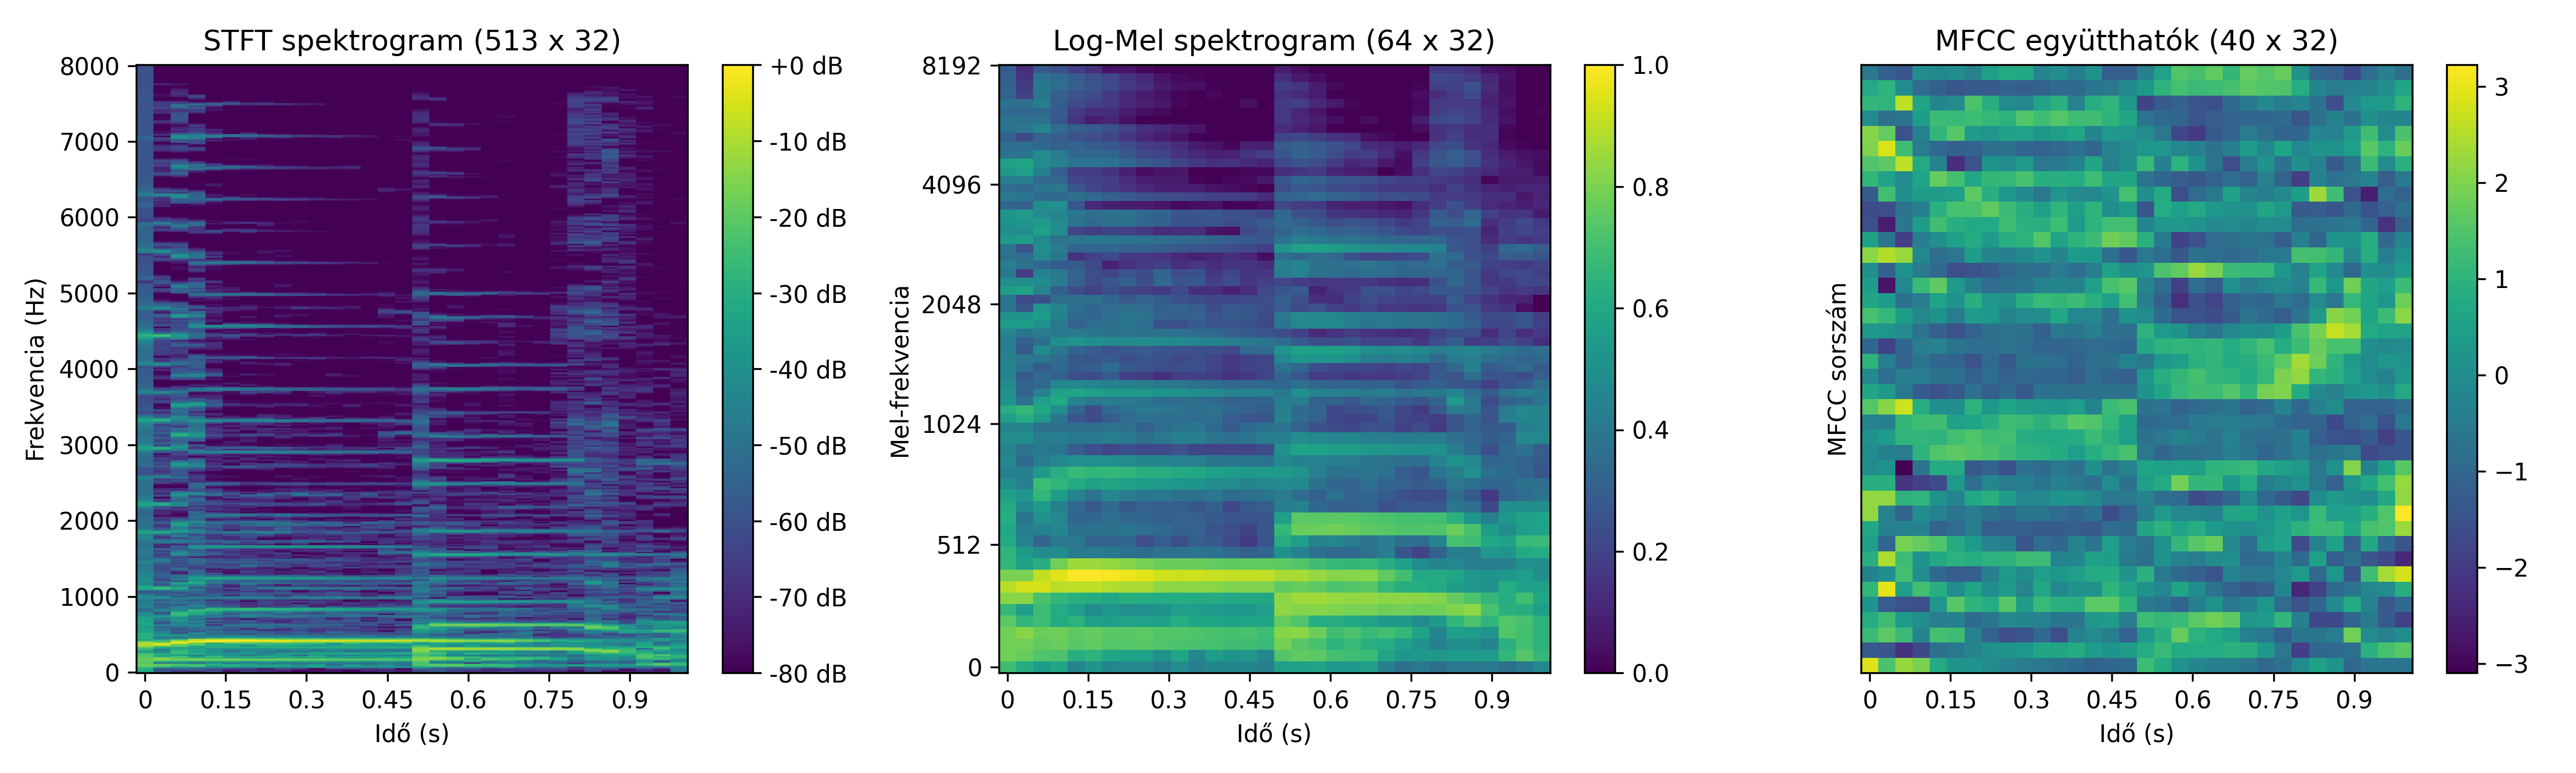
\includegraphics[width=\textwidth]{fig_feature_comparison.png}
  \caption{A három vizsgált jellemzőtípus vizualizációja ugyanazon gitárminta esetén: (a) STFT spektrogram ($513 \times 32$), (b) normalizált Log-Mel spektrogram ($64 \times 32$), (c) normalizált MFCC együtthatók ($40 \times 32$)}
  \label{fig:feature_comparison}
\end{figure}

\subsection{Jellemzőkinyerés kimeneti állományai}
\label{subsec:feature_outputs}

A jellemzőkinyerési folyamat sikeres lefutása után a kinyert mátrixok és a hozzájuk tartozó osztálycímkék a projekt gyökerében lévő \texttt{processed\_data\_clean/} és \texttt{processed\_data\_mic/} könyvtárakba kerülnek elmentésre NumPy formátumban (\texttt{.npy} kiterjesztéssel), az alkalmazott forrásadathalmaztól függően. A generált fájlok már nem egyetlen nagy tömbben, hanem a szeparált kiértékelési halmazoknak megfelelően szétbontva (\texttt{train}, \texttt{val}, \texttt{test}) készülnek el. Például a \texttt{train} halmazhoz tartozó fájlok a következők:
\begin{itemize}
  \item \textbf{Log-Mel spektrogram:} \texttt{X\_log\_mel\_train.npy} (a jellemzőmátrixokat tartalmazó tömb) és \texttt{y\_labels\_train.npy} (a hangszerosztályok sorszámait tartalmazó címketömb),
  \item \textbf{STFT spektrogram:} \texttt{X\_stft\_train.npy},
  \item \textbf{MFCC együtthatók:} \texttt{X\_mfcc\_train.npy},
  \item \textbf{Nyers hanghullám (csak a mic adathalmaznál):} \texttt{X\_raw\_train.npy}, amely az olyan transzfer tanulási architektúrák, mint a YAMNet, közvetlen bemeneteként szolgál.
\end{itemize}
A normalizált és binárisan tömörített fájlformátum biztosítja, hogy a tanítási fázisban a minták betöltése rendkívül gyorsan, közvetlenül a memóriába (RAM) történhessen meg, elkerülve a felesleges lemezműveleteket.

%% ═══════════════════════════════════════════════════════════════════════════
\section{Adataugmentáció tervezése}
\label{sec:augmentation}

A modell valós idejű kiértékelésre való felkészítése érdekében a tanító (train) halmaz minden tiszta hangszermintáját (a noise osztályt és az eleve mikrofonnal rögzített \texttt{\_mic\_} mintákat kivéve) egy augmentált változattal egészítek ki. Az augmentáció a fogyasztói mikrofonos felvétel körülményeit szimulálja, ezért a belső elnevezése \texttt{apply\_macbook\_\allowbreak augment}. Az alkalmazott adataugmentációs lánc felépítését és a lépések sorrendjét a \ref{fig:augmentation_chain}.~ábrán mutatom be, míg az augmentáció hatását a spektrális jellemzőkre (egy gitárminta példáján keresztül) a \ref{fig:original_vs_augmented}.~ábra szemlélteti.

Az augmentációs lánc a következő lépésekből áll:

\subsection{Szobai reverb szimuláció}
\label{subsec:reverb}

A reverb szimulációt 80\%-os valószínűséggel alkalmazom. A szoba akusztikáját egy egyszerű FIR visszhang-modellel közelítem, amely négy visszaverődési pontot (tap) használ:

\begin{itemize}
  \item Késleltetés (\textit{delay}): véletlenszerű, 15--40 ms között,
  \item Csillapítási tényező (\textit{decay}): véletlenszerű, 0{,}2--0{,}45 között,
  \item Visszaverődési pontok: $d$, $1{,}5d$, $2{,}1d$, $2{,}8d$ mintányi késleltetésnél,
  \item Csillapítás: $decay^1$, $decay^2$, $decay^3$, $decay^4$.
\end{itemize}

\subsection{Frekvenciaválasz-torzítás (Pre-emphasis)}

A mikrofon és a szoba együttes frekvenciaválaszának szimulálására pre-emphasis szűrőt alkalmazok, amelynek együtthatója véletlenszerűen 0{,}92 és 0{,}98 között változik:

$$y[n] = x[n] - \alpha \cdot x[n-1]$$

\subsection{Környezeti zajkeverés (Noise mixing)}

A háttérzajt az ESC-50 adathalmaz~\cite{piczak2015esc} véletlenszerűen kiválasztott zajmintájával keverem a hangszermintához. A keverési arány (SNR) véletlenszerűen 5--15~dB között változik:

$$y_{mixed} = x_{clean} + \sqrt{\frac{P_{clean}}{SNR_{lin} \cdot P_{noise}}} \cdot x_{noise}$$

ahol $SNR_{lin} = 10^{SNR_{dB}/10}$, és $P$ a jel átlagos teljesítménye.

\subsection{Szoftklip torzítás (Soft clipping)}

A mikrofon bemeneti erősítőjének telítési karakterisztikáját hiperbolikus tangens szoftklippel modellezem:

$$y[n] = \frac{\tanh(drive \cdot x[n])}{\tanh(drive)}$$

ahol $drive$ véletlenszerűen 2{,}0 és 4{,}0 között változik.

\subsection{Végső normalizálás}

Az augmentált jelet csúcsértékre normalizálom, hogy az amplitúdó ne haladja meg a 0{,}9-es szintet:

$$y_{norm} = \frac{y}{\max(|y|)} \cdot 0{,}9$$

\begin{figure}[H]
\centering
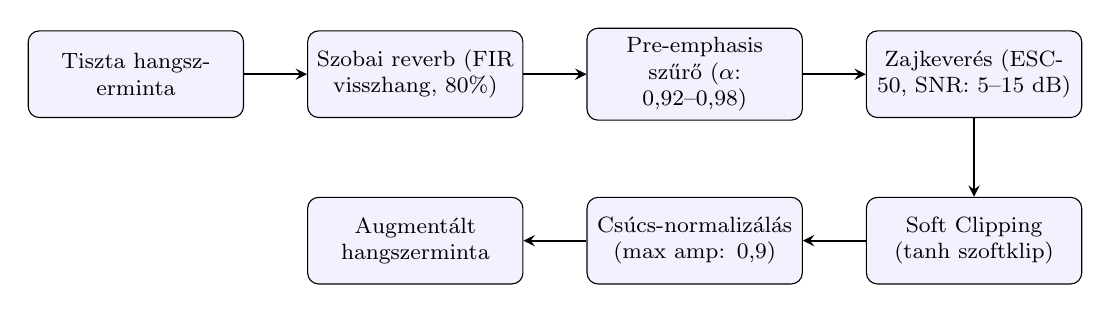
\begin{tikzpicture}[
    node distance=1.0cm and 0.8cm,
    block/.style={draw, rectangle, minimum height=1.1cm, minimum width=2.6cm, fill=blue!5!white, text width=2.5cm, align=center, font=\footnotesize, rounded corners},
    arrow/.style={thick,->,>=stealth}
]
  % Nodes Row 1
  \node (orig) [block] {Tiszta hangszerminta};
  \node (reverb) [block, right=0.8cm of orig] {Szobai reverb (FIR visszhang, 80\%)};
  \node (preemph) [block, right=0.8cm of reverb] {Pre-emphasis szűrő ($\alpha$: 0,92--0,98)};
  \node (noise) [block, right=0.8cm of preemph] {Zajkeverés (ESC-50, SNR: 5--15 dB)};
  
  % Nodes Row 2
  \node (clip) [block, below=1.0cm of noise] {Soft Clipping ($\tanh$ szoftklip)};
  \node (norm) [block, left=0.8cm of clip] {Csúcs-normalizálás (max amp: 0,9)};
  \node (aug) [block, left=0.8cm of norm] {Augmentált hangszerminta};
  
  % Arrows
  \draw [arrow] (orig) -- (reverb);
  \draw [arrow] (reverb) -- (preemph);
  \draw [arrow] (preemph) -- (noise);
  \draw [arrow] (noise) -- (clip);
  \draw [arrow] (clip) -- (norm);
  \draw [arrow] (norm) -- (aug);
\end{tikzpicture}
\caption{A MacBook/mikrofonos felvételi körülményeket szimuláló adataugmentációs folyamatlánc}
\label{fig:augmentation_chain}
\end{figure}

\begin{figure}[H]
  \centering
  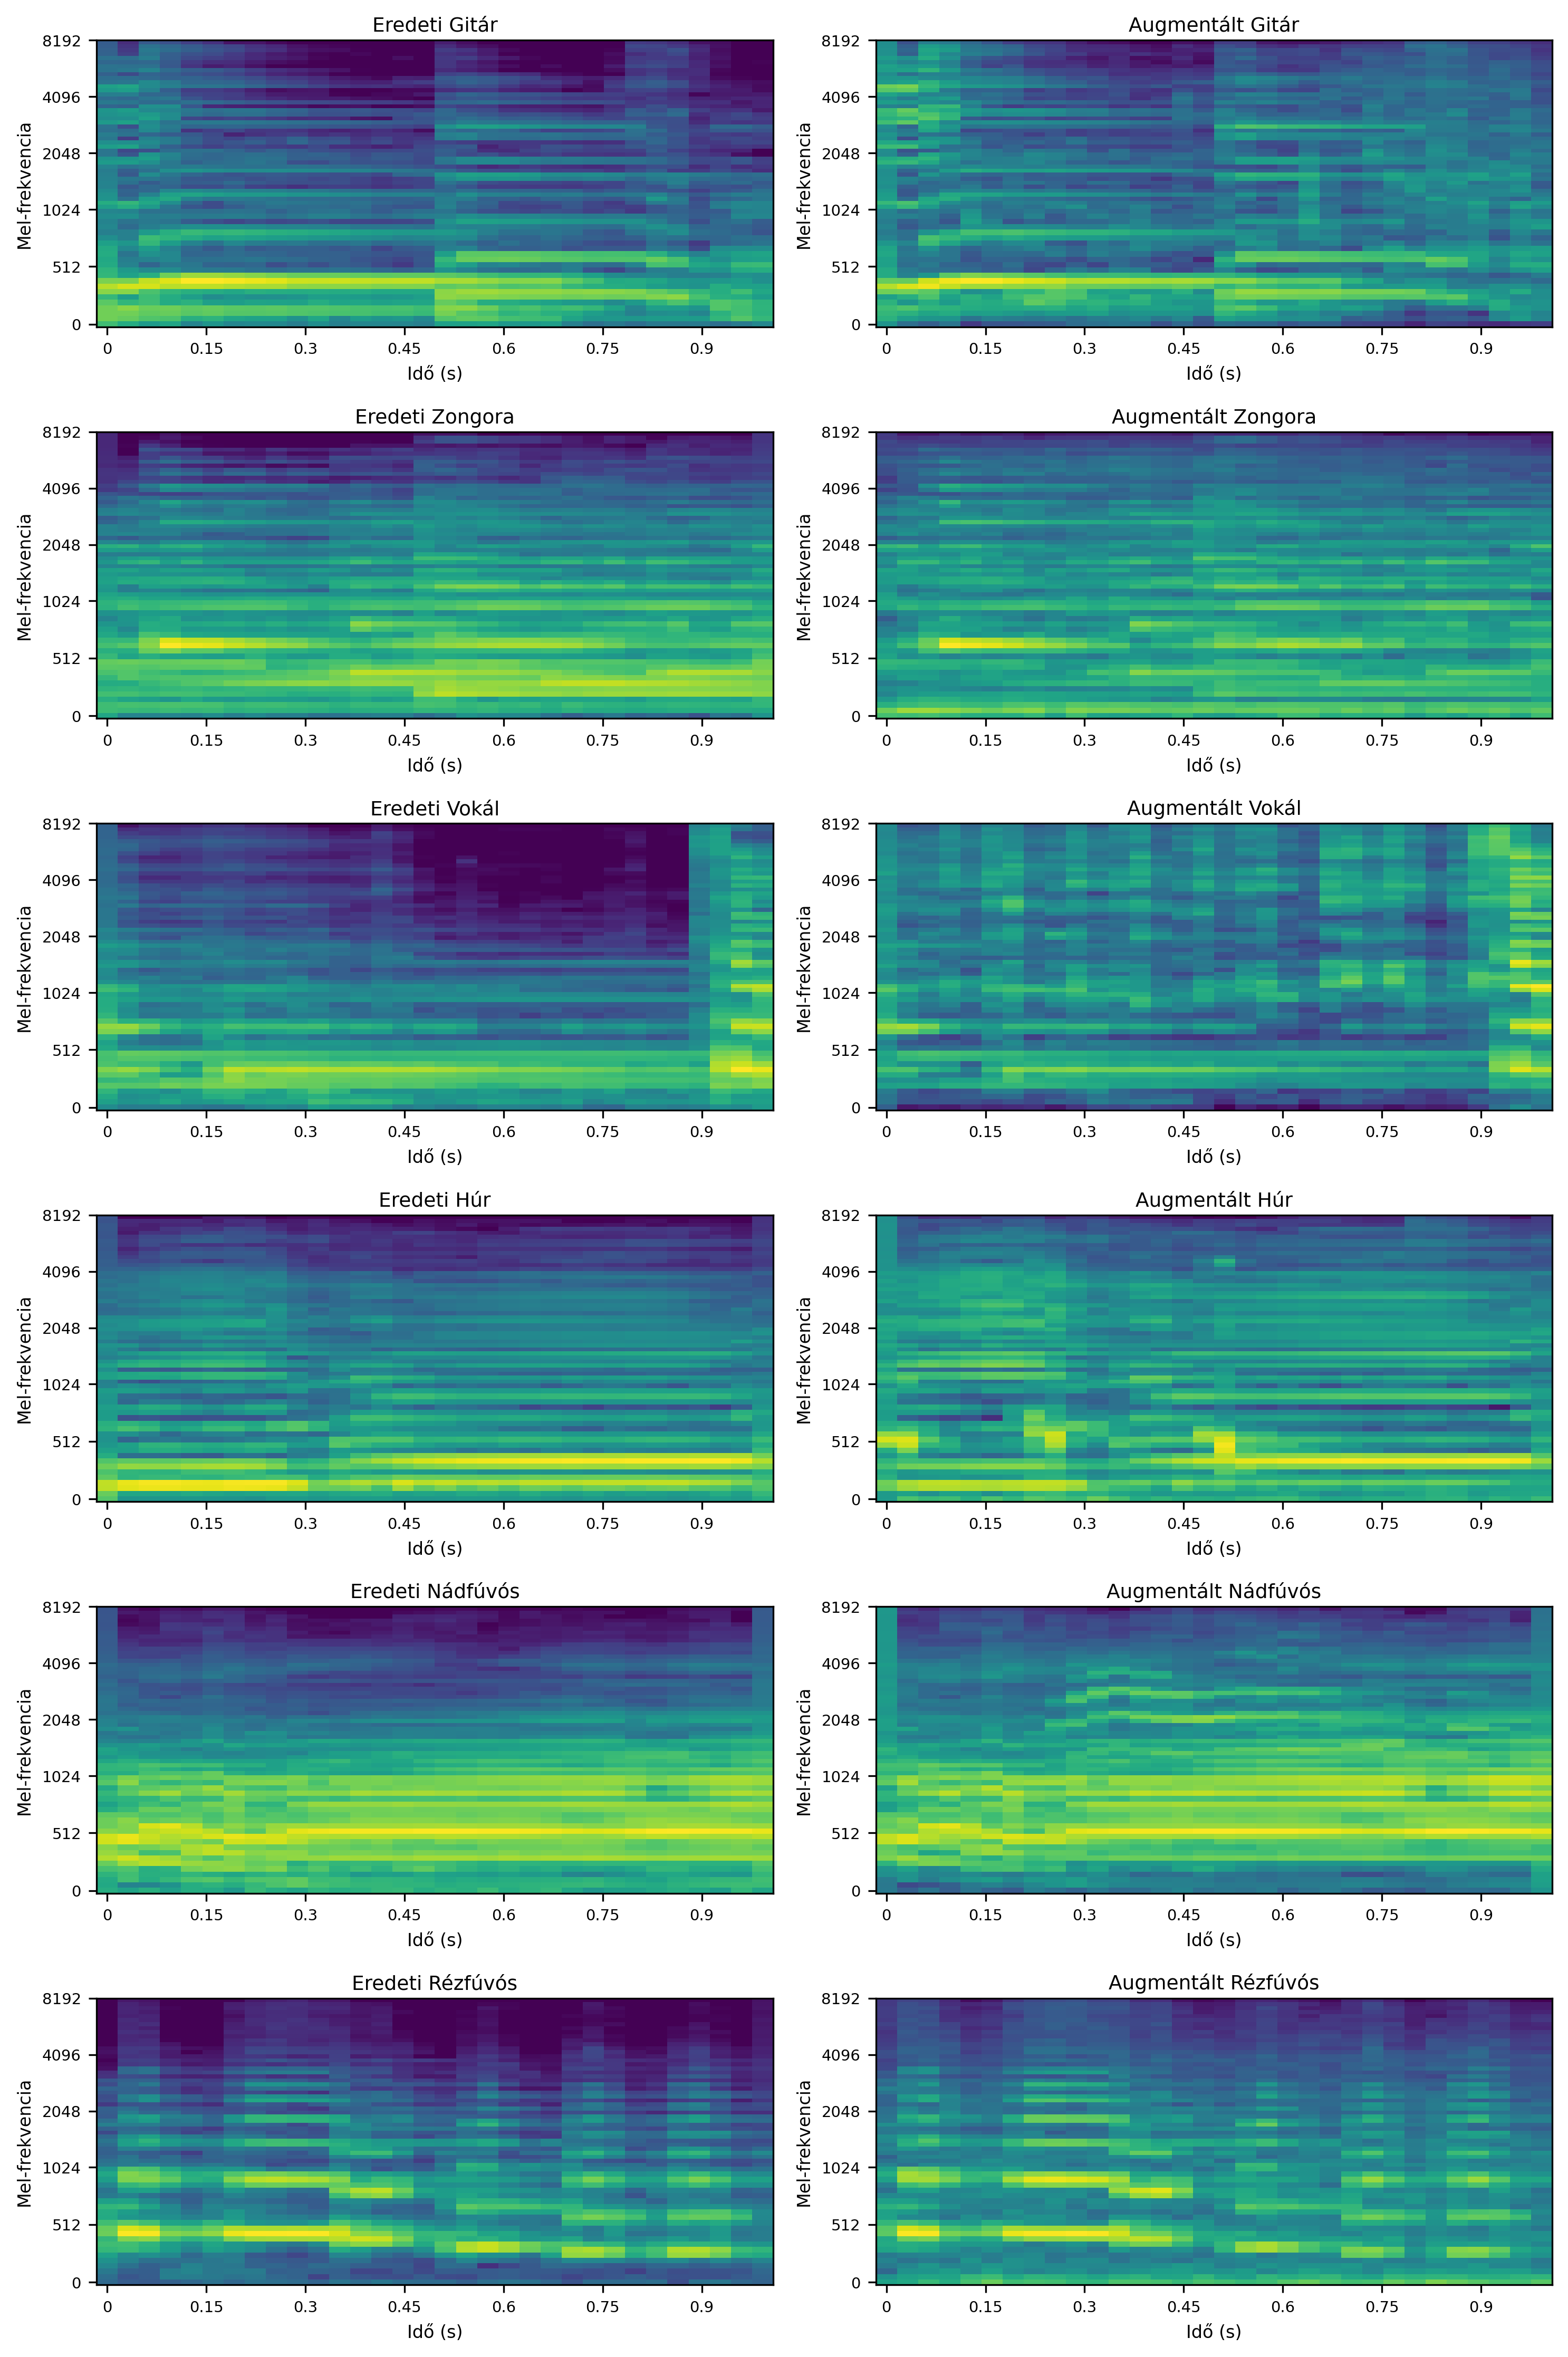
\includegraphics[height=0.74\textheight,keepaspectratio]{fig_original_vs_augmented.png}
  \caption{A hat hangszerosztály (gitár, zongora, vokál, hegedű, klarinét, kürt) egy-egy reprezentatív mintájának normalizált Log-Mel spektrogramja az eredeti (tiszta) és az adataugmentált (MacBook/mikrofon szimulációs lánccal torzított) állapotban}
  \label{fig:original_vs_augmented}
\end{figure}

Az augmentáció eredményeként a 6 hangszerosztály \textbf{tanító (train) halmazának tiszta mintái} kiegészülnek egy-egy torzított változattal (a \texttt{noise} és a már eleve mikrofonnal rögzített \texttt{\_mic\_} mintákat a script logikája automatikusan kihagyja).

Az augmentációs eljárás helyességének és minőségének manuális ellenőrzése, illetve összehasonlítása céljából a rendszer minden hangszerosztályból kiment néhány bemutató mintát (az eredeti és az augmentált változat párosait) az \texttt{augmented\_preview/} könyvtárba. Ez a gyakorlatban lehetővé teszi a fejlesztő számára, hogy mind füllel (hallás útján), mind vizuálisan meggyőződjön arról, hogy az alkalmazott szimulációs torzítások (például visszhang és zajkeverés) valósághűek, és nem teszik felismerhetetlenné a hangszerek alapvető karakterét.

%% ═══════════════════════════════════════════════════════════════════════════
\section{Modell architektúrák tervezése}
\label{sec:cnn_architecture}

A tervezett hangszerfelismerő rendszer magját egy mély konvolúciós neurális hálózat (CNN) alkotja, amely a Log-Mel spektrogramok 2D-s vizuális mintázatait tanulja meg osztályozni. Ebben a fejezetben részletezem a hálózat felépítését, a rétegek sorrendjét és paramétereit, valamint a hálózat betanításához használt konfigurációkat. A tervezett hálózati rétegek specifikációit a \ref{tab:cnn_standard}.~táblázat foglalja össze, a rétegek közötti adatfolyamot és az architektúra grafikus felépítését pedig a \ref{fig:cnn_architecture}.~ábra ábrázolja.

\subsection{A hálózati architektúra részletei}
\label{subsec:cnn_details}

A rendszer magját egy VGG-stílusú, háromblokkos konvolúciós hálózat (2D CNN) alkotja, kiegészítve egy bemeneti SpecAugment réteggel. A SpecAugment menet közben véletlenszerű idő- és frekvenciamaszkolással takar ki részleteket a spektrogramból, így kényszerítve a hálózatot az átfogóbb mintázatok megtanulására és a túlilleszkedés (overfitting) elkerülésére. A konvolúciós blokkok két egymást követő 2D konvolúcióból, Batch Normalization-ből, ReLU aktivációból, majd végül Max Poolingból és Dropoutból (30\%) állnak. A hálózat bemenete a kiválasztott, normalizált Log-Mel spektrogram ($64 \times 32 \times 1$), a kimenetnél pedig a hagyományos Flatten helyett térbeli átlagolást (GlobalAveragePooling2D) alkalmazunk a paraméterszám drasztikus csökkentése érdekében.

\begin{table}[H]
\centering
\caption{A tervezett 2D CNN architektúra rétegei (Log-Mel bemenet: $64 \times 32 \times 1$)}
\label{tab:cnn_standard}
\resizebox{\textwidth}{!}{
\begin{tabular}{llll}
\toprule
\textbf{Réteg} & \textbf{Szűrők / Neuronok} & \textbf{Kimenet} & \textbf{Paraméterek} \\
\midrule
SpecAugment & max 15 frekvencia, 8 idő maszk & $64 \times 32 \times 1$ & 0 \\
\midrule
2$\times$ Conv2D+BN+ReLU & 32 szűrő, $3 \times 3$, same & $64 \times 32 \times 32$ & $320 + 128 + 9\,248 + 128$ \\
MaxPool2D + Dropout & $2 \times 2$, dropout: 0{,}3 & $32 \times 16 \times 32$ & 0 \\
\midrule
2$\times$ Conv2D+BN+ReLU & 64 szűrő, $3 \times 3$, same & $32 \times 16 \times 64$ & $18\,496 + 256 + 36\,928 + 256$ \\
MaxPool2D + Dropout & $2 \times 2$, dropout: 0{,}3 & $16 \times 8 \times 64$ & 0 \\
\midrule
2$\times$ Conv2D+BN+ReLU & 128 szűrő, $3 \times 3$, same & $16 \times 8 \times 128$ & $73\,856 + 512 + 147\,584 + 512$ \\
GlobalAvgPool2D + Drop & dropout: 0{,}5 & 128 & 0 \\
\midrule
Dense + BN + ReLU & 128 neuron & 128 & $16\,512 + 512$ \\
Dropout & 0{,}5 & 128 & 0 \\
Dense & 7, Softmax & 7 & 903 \\
\midrule
\textbf{Összesen} & & & $\sim$306\,150 \\
\bottomrule
\end{tabular}
}
\end{table}

\begin{figure}[H]
\centering
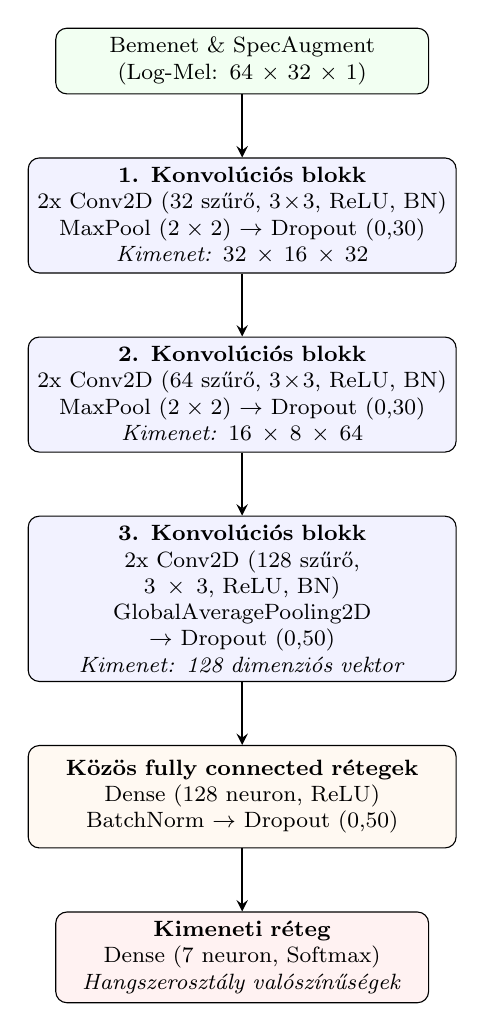
\begin{tikzpicture}[
    node distance=0.8cm and 0.5cm,
    layer/.style={draw, rectangle, minimum height=0.8cm, minimum width=3.5cm, align=center, font=\footnotesize, rounded corners},
    input/.style={layer, fill=green!5!white, text width=4.5cm},
    block/.style={layer, fill=blue!5!white, text width=5.2cm, minimum height=1.3cm},
    dense/.style={layer, fill=orange!5!white, text width=5.2cm, minimum height=1.3cm},
    output/.style={layer, fill=red!5!white, text width=4.5cm},
    arrow/.style={thick,->,>=stealth}
]
  % Nodes
  \node (input) [input] {Bemenet \& SpecAugment \\ (Log-Mel: $64 \times 32 \times 1$)};
  
  \node (block1) [block, below=of input] {\textbf{1. Konvolúciós blokk} \\ 2x Conv2D (32 szűrő, $3\times3$, ReLU, BN) \\ MaxPool ($2\times2$) $\rightarrow$ Dropout (0,30) \\ \textit{Kimenet: $32 \times 16 \times 32$}};
  
  \node (block2) [block, below=of block1] {\textbf{2. Konvolúciós blokk} \\ 2x Conv2D (64 szűrő, $3\times3$, ReLU, BN) \\ MaxPool ($2\times2$) $\rightarrow$ Dropout (0,30) \\ \textit{Kimenet: $16 \times 8 \times 64$}};
  
  \node (block3) [block, below=of block2] {\textbf{3. Konvolúciós blokk} \\ 2x Conv2D (128 szűrő, $3\times3$, ReLU, BN) \\ GlobalAveragePooling2D $\rightarrow$ Dropout (0,50) \\ \textit{Kimenet: 128 dimenziós vektor}};
  
  \node (flatten) [dense, below=of block3] {\textbf{Közös fully connected rétegek} \\ Dense (128 neuron, ReLU) \\ BatchNorm $\rightarrow$ Dropout (0,50)};
  
  \node (output) [output, below=of flatten] {\textbf{Kimeneti réteg} \\ Dense (7 neuron, Softmax) \\ \textit{Hangszerosztály valószínűségek}};
  
  % Arrows
  \draw [arrow] (input) -- (block1);
  \draw [arrow] (block1) -- (block2);
  \draw [arrow] (block2) -- (block3);
  \draw [arrow] (block3) -- (flatten);
  \draw [arrow] (flatten) -- (output);
\end{tikzpicture}
\caption{A tervezett 2D CNN hálózati architektúra felépítése és adatfolyama}
\label{fig:cnn_architecture}
\end{figure}



\subsection{YAMNet Transfer Learning architektúra}
\label{subsec:yamnet_architecture}

Bár a saját fejlesztésű 2D CNN hálózat stabil teljesítményt nyújt (78\%-os baseline pontosság), a valós környezet sokrétű zajai és a felvételi torzítások kihívásai miatt szükség volt egy még stabilabb, jobban általánosító modellre. Ennek eléréséhez a Google által fejlesztett és a TensorFlow Hub-on publikált YAMNet modellt választottam ki. 

A YAMNet egy mély, MobileNetV1 alapú architektúra, amelyet a hatalmas AudioSet adatbázison tanítottak be, így kiváló akusztikai reprezentációs képességekkel rendelkezik. A YAMNet bemenete közvetlenül a normalizált nyers hanghullám ($16\,000$ elemű vektor).

A rendszeremben a YAMNet modellt nem a nulláról tanítom újra, hanem jellemzőkinyerőként (feature extractor) használom. A folyamat során az 1 másodperces audiojel végighalad a YAMNet befagyasztott konvolúciós rétegein, aminek az eredménye egy 1024 dimenziós sűrű reprezentáció (beágyazás, azaz \textit{embedding}). 

Ezt a mély beágyazást egy saját tervezésű, teljesen összekapcsolt (fully connected) osztályozó hálózatba vezetem be. Az általam tervezett osztályozó felépítése a következő:
\begin{enumerate}
  \item \textbf{Bemenet:} 1024 dimenziós YAMNet embedding
  \item \textbf{Rejtett réteg 1:} Sűrű réteg (Dense), 256 neuron, ReLU aktiváció
  \item \textbf{Normalizáció 1:} Batch Normalization és 40\% Dropout
  \item \textbf{Rejtett réteg 2:} Sűrű réteg (Dense), 128 neuron, ReLU aktiváció
  \item \textbf{Normalizáció 2:} Batch Normalization és 40\% Dropout
  \item \textbf{Kimeneti réteg:} Sűrű réteg (Dense), 7 neuron, Softmax aktiváció (hangszerosztályok valószínűségei)
\end{enumerate}

Ez az architektúra nemcsak, hogy drasztikus pontosságnövekedést (akár 90\% körüli F1-score) és sokkal stabilabb működést eredményezett a saját CNN baseline-hoz képest, de a tanítási időt is jelentősen lecsökkentette.

\subsection{Tanítási konfiguráció}


A 2D CNN modell tanítása során alkalmazott konfigurációt és hiperparamétereket úgy válogattam meg, hogy biztosítsák a modell stabil konvergenciáját és elkerüljék a túlilleszkedést (overfitting), miközben hatékonyan kihasználják a rendelkezésre álló számítási erőforrásokat. A modell optimalizálását, a veszteségfüggvényt, az adathalmaz felosztását és a tanulási folyamatot szabályozó callback mechanizmusokat a \ref{tab:training_config}.~táblázat foglalja össze részletesen.

\begin{table}[H]
\centering
\caption{A modell tanításához használt konfigurációs paraméterek és beállítások}
\label{tab:training_config}
\begin{tabular}{lp{8.0cm}}
\toprule
\textbf{Paraméter / Beállítás} & \textbf{Érték / Részletek} \\
\midrule
Optimalizáló & AdamW (tanulási ráta: $10^{-3}$, weight decay: $10^{-4}$) \\
Veszteségfüggvény & Categorical Crossentropy (Label Smoothing: 0,1 alkalmazásával) \\
Tanító/validációs/teszt & 70\% / 15\% / 15\% (rétegzett felosztásban) \\
Batch méret & 32 \\
Maximális epochszám & 150 \\
Early Stopping & \texttt{val\_loss} monitorozás, patience = 10, legjobb súlyok visszaállítása (\texttt{restore\_best\_weights=True}) \\
ReduceLROnPlateau & \texttt{val\_loss} monitorozás, patience = 4, faktor = 0{,}5, minimális tanulási ráta: $10^{-6}$ \\
ModelCheckpoint & \texttt{val\_accuracy} alapján a legjobb modell mentése \texttt{.keras} formátumban \\
\bottomrule
\end{tabular}
\end{table}

A táblázatban szereplő beállítások elméleti háttere és működési célja a következő:
\begin{itemize}
  \item \textbf{AdamW optimalizáló és Címkesimítás (Label Smoothing):} A hagyományos Adam helyett az AdamW optimalizálót (súlycsökkenés / weight decay bevonásával), a veszteségfüggvénynél pedig 0,1-es címkesimítást alkalmaztam. Ez a két technika együttesen erősen bünteti a modell túlzott magabiztosságát (overconfidence), ezáltal nagymértékben megelőzve a túlilleszkedést a zajos hangmintáknál.
  \item \textbf{Early Stopping callback:} Megakadályozza az iterációk felesleges futását. Ha a validációs veszteség (\texttt{val\_loss}) 10 egymást követő epochoz tartozóan már nem csökken, a tanítási folyamat automatikusan leáll, és visszaállítja a modellt a legjobb állapotba.
  \item \textbf{ReduceLROnPlateau callback:} Lehetővé teszi a tanulási ráta menet közbeni finomhangolását. Ha a modell elakad egy lokális minimum közelében (azaz a \texttt{val\_loss} nem csökken 4 epoch óta), a tanulási sebességet lefelezi ($0{,}5$-ös faktor), így segítve a precízebb konvergenciát.
\end{itemize}

A tanítás a Google Colab felhőszolgáltatás GPU-ján történik, az adatokat és a mentett modelleket a Google Drive-on tároljuk és onnan töltjük vissza a projektbe.

\subsubsection{A tanítás során generált kimenetek}
\label{subsubsec:model_outputs}

A tanítás lefutását követően a validációs adathalmazon legjobban teljesítő modellállapotok a projekt gyökerében lévő \texttt{models/} könyvtárba kerülnek mentésre. A különböző jellemzőtípusok alapján a következő fájlok jönnek létre:
\begin{itemize}
  \item \textbf{Log-Mel alapú CNN modell:} \texttt{best\_log\_mel\_2dcnn\_model.keras},
  \item \textbf{STFT alapú CNN modell:} \texttt{best\_stft\_2dcnn\_model.keras},
  \item \textbf{MFCC alapú CNN modell:} \texttt{best\_mfcc\_2dcnn\_model.keras}.
\end{itemize}
A TensorFlow \texttt{.keras} formátuma magában foglalja a hálózat architektúráját, a betanult súlymátrixokat, valamint az optimalizáló állapotát is. Ezen kimenetek közvetlenül betölthetőek a \texttt{tf.keras.models.load\_model} függvény segítségével, ami lehetővé teszi, hogy a valós idejű felismerő modul másodpercek alatt elinduljon a korábban elmentett legjobb modellállapot betöltésével.


%% ═══════════════════════════════════════════════════════════════════════════
\section{A valós idejű felismerő modul tervezése}
\label{sec:realtime}

A valós idejű hangszerfelismerő modul célja, hogy a számítógép mikrofonján keresztül érkező folyamatos audiojelet valós időben dolgozza fel, és minimális késleltetéssel jelezze ki a felismert hangszert és a predikció konfidenciaértékét. A modul stabil, aszinkron működésének megvalósításához egy többszálú architektúrát és egy egyedi predikciós stabilizáló logikát terveztem.

\subsection{Audio stream és aszinkron pufferelés}

A valós idejű hangfelvétel és a jelfeldolgozási lépések szétválasztásához többszálú jelfeldolgozó láncot alkalmazok. A hangkártya fizikai bemenetének kezeléséért a \texttt{sounddevice} könyvtár \texttt{InputStream} API-ja felel, amely egy magas prioritású háttérszálon futó hardveres megszakítási visszahívásos (callback) mechanizmusra épül:

\begin{itemize}
  \item \textbf{Mintavételi frekvencia ($f_s$):} 16\,000~Hz,
  \item \textbf{Csatornaszám:} 1 (monó),
  \item \textbf{Lépésköz (Step duration):} $0,25$ másodperc (4000 minta).
\end{itemize}

A beérkező audioadatok kezelése egy szálbiztos FIFO soron (\texttt{queue.Queue}) keresztül történik. Az audio callback függvény kizárólag a hardver pufferéből érkező 4000 mintás csomagokat helyezi el a sorban, majd azonnal visszatér. Ez garantálja, hogy a CPU-igényes neurális hálózati következtetés és a terminálfrissítés nem blokkolja a hangkártya illesztőprogramját, elkerülve az audió puffer alulcsordulását (buffer underflow).

A fő feldolgozó szál folyamatosan olvassa a sorból a 0,25 másodperces blokkokat. A predikció alapját egy folyamatos, $1,0$ másodperces (16\,000 minta) csúszóablak képezi. A 75\%-os átfedés (overlap) eléréséhez egy körpuffer-szerű logikát alkalmazok: minden új 0,25 másodperces blokk beérkezésekor a puffer tartalmát balra csúsztatom 4000 mintával, és az új adatot a puffer végére írom (roll művelet). Ezáltal a rendszer másodpercenként négyszer hajt végre predikciót az utolsó 1 másodpercnyi hanganyagra vonatkozóan.

\subsection{Jellemzőkinyerés és normalizálás}

A felismerő rendszer alapvetően kétféle hálózattal tud elindulni. Amennyiben a saját fejlesztésű 2D CNN hálózatot használjuk, minden predikciós ciklusban az 1 másodperces pufferből kinyerem a Log-Mel spektrogram jellemzőket. A kinyert spektrális mátrix dimenziója $128 \times 63$, ami megegyezik a tanítás során használt bemenettel.

A 2D CNN bemeneti rétege $[0, 1]$ intervallumba skálázott adatokat vár. A valós idejű jellemzőkre a tanítási fázissal azonos normalizálást alkalmazok decibel alapú korlátokkal:
$$X_{\text{norm}} = \frac{X_{\text{dB}} + 80,0}{80,0}$$
A kapott értékeket a $[0, 1]$ intervallumra vágom le (\texttt{clip} művelet), majd a tenzort átformázom a $1 \times 128 \times 63 \times 1$ bemeneti formára (batch és csatorna dimenziók hozzáadásával).

A fejlettebb, YAMNet alapú felismerő modul esetében az eljárás jóval egyszerűbb: a teljes, 16\,000 mintás nyers audiopuffert közvetlenül átalakítjuk TensorFlow tenzorrá, amiből a lefagyasztott YAMNet elkészíti az 1024-es beágyazást (embedding). Ezt az embedding vektort kapja meg a saját betanított osztályozónk.

\subsection{Zaj-alapú küszöbölés és Predikciós stabilizáció}

A hangszerosztályok pillanatnyi valószínűségei a zenefájlokban és az élő játékban tapasztalható dinamikus változások (tranziensek, vibrato, környezeti zajok) miatt gyorsan ingadozhatnak. Ha közvetlenül az aktuális predikció legnagyobb valószínűségű osztályát jelenítenénk meg, a terminálon zavaró, gyors váltások (,,villogás'') jelennének meg. Ennek kiszűrésére egy összetett stabilizációs logikát terveztem:

\begin{enumerate}
  \item \textbf{Temporális mozgóátlag simítás:} A modell kimeneti valószínűség-vektorait egy $W = 6$ elemű FIFO sorban tárolom (amely a 250 ms-os lépésköz miatt az utolsó $1,5$ másodperc predikciós történetét fedi le). A döntéshozatal a simított valószínűség-vektor alapján történik:
  $$\bar{p}_c^{(t)} = \frac{1}{W} \sum_{i=0}^{W-1} p_c^{(t-i)}$$
  
  \item \textbf{Hiszterézis mechanizmus:} Annak érdekében, hogy megakadályozzuk a két közeli valószínűségű osztály közötti ugrálást (chattering), egy $H = 0,05$ ($5\%$) értékű hiszterézis bónuszt adunk a jelenleg aktív (kijelzett) osztály $C^{(t-1)}$ simított valószínűségéhez a maximumkeresés előtt:
  $$a_c^{(t)} = \bar{p}_c^{(t)} + H \cdot \mathbb{I}(c = C^{(t-1)})$$
  ahol $\mathbb{I}$ az indikátorfüggvény. A jelölt új osztályt a módosított vektor maximumhelye adja meg.
  
  \item \textbf{Osztály-specifikus konfidencia-küszöb:} Nem alkalmazok fix hardveres RMS alapú zajkaput, mivel a modell kiválóan megtanulta a \texttt{noise} (zaj/csend) osztály felismerését. Helyette a predikció során osztály-specifikus küszöbértékeket ellenőrzök, amelyek értékeit az alábbi empirikus megfontolások alapján határoztam meg:
  \begin{itemize}
      \item \textbf{Hangszerek küszöbe ($45\%$):} Mivel 7 kategóriánk van, egy teljesen véletlenszerű döntés $\sim$14\%-os valószínűséget jelentene. A 45\%-os küszöb megköveteli, hogy a modell határozottan dominánsnak ítélje meg a felismert hangszert. Ezzel elkerülhetők a vakriasztások (false positives), amik a zajosabb tranziensek vagy műfajok közötti átmenetek során 20-30\%-os tüskeként jelentkezhetnének.
      \item \textbf{Zaj/Csend küszöbe ($20\%$):} Amikor a hangszeres játék befejeződik, a mikrofonba csak a szoba alapzaja jut. Ilyenkor a neurális hálózat gyakran bizonytalanabb, és a kimeneti valószínűséget szétkeni a többi 6 osztály között, így a \texttt{noise} kimenet ritkán éri el a 45\%-ot. Ha a zajhoz is magas küszöböt követelnénk, a kijelző "beleragadna" az utolsó hangszer állapotába. A mindössze 20\%-os (de még mindig az egyenletes eloszlásnál magasabb) küszöb biztosítja, hogy a rendszer agresszívan és gyorsan visszaálljon az alapállapotra (csendre), amint a hangszer elhalkul.
  \end{itemize}
  A kijelzett hangszercsere tehát csak akkor történik meg, ha a vizsgált osztály simított valószínűsége átlépi a rá vonatkozó küszöböt. Ez a szoftveres megoldás feleslegessé teszi a jelszint alapú RMS számítást.
\end{enumerate}

Ez a tervezési megoldás rendkívül stabil vizuális visszajelzést biztosít a felhasználói felületen, miközben a gyorsabb, 0,25 másodperces frissítési ütemnek köszönhetően a rendszer rendkívül reszponzív marad. A valós idejű felismerési folyamat egyes lépéseit a \ref{fig:realtime_pipeline}.~ábra foglalja össze vizuálisan.

\begin{figure}[H]
\centering
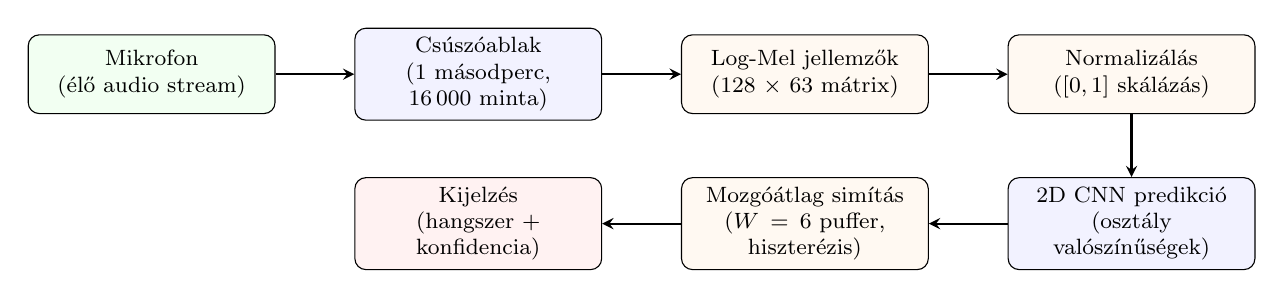
\begin{tikzpicture}[
    node distance=0.8cm and 1.0cm,
    flowblock/.style={draw, rectangle, minimum height=1.0cm, minimum width=3.0cm, fill=blue!5!white, align=center, font=\footnotesize, rounded corners, text width=2.9cm},
    flowio/.style={draw, rectangle, minimum height=1.0cm, minimum width=3.0cm, fill=green!5!white, align=center, font=\footnotesize, rounded corners, text width=2.9cm},
    flowproc/.style={draw, rectangle, minimum height=1.0cm, minimum width=3.0cm, fill=orange!5!white, align=center, font=\footnotesize, rounded corners, text width=2.9cm},
    flowout/.style={draw, rectangle, minimum height=1.0cm, minimum width=3.0cm, fill=red!5!white, align=center, font=\footnotesize, rounded corners, text width=2.9cm},
    flowarrow/.style={thick,->,>=stealth}
]
  % Nodes
  \node (mic) [flowio] {Mikrofon \\ (élő audio stream)};
  \node (seg) [flowblock, right=of mic] {Csúszóablak \\ (1 másodperc, 16\,000 minta)};
  \node (mel) [flowproc, right=of seg] {Log-Mel jellemzők \\ (128 $\times$ 63 mátrix)};
  \node (norm) [flowproc, right=of mel] {Normalizálás \\ ($[0,1]$ skálázás)};
  
  \node (cnn) [flowblock, below=of norm] {2D CNN predikció \\ (osztály valószínűségek)};
  \node (avg) [flowproc, left=of cnn] {Mozgóátlag simítás \\ ($W=6$ puffer, hiszterézis)};
  \node (disp) [flowout, left=of avg] {Kijelzés \\ (hangszer + konfidencia)};
  
  % Arrows
  \draw [flowarrow] (mic) -- (seg);
  \draw [flowarrow] (seg) -- (mel);
  \draw [flowarrow] (mel) -- (norm);
  \draw [flowarrow] (norm) -- (cnn);
  \draw [flowarrow] (cnn) -- (avg);
  \draw [flowarrow] (avg) -- (disp);
\end{tikzpicture}
\caption{A valós idejű felismerési folyamat lépései az élő hangbeviteltől a kijelzésig}
\label{fig:realtime_pipeline}
\end{figure}

%% ═══════════════════════════════════════════════════════════════════════════
\section{A feldolgozási folyamat összefoglaló áttekintése}
\label{sec:pipeline_overview}

A teljes rendszer a tervezéstől a megvalósításig egymásra épülő fázisokból áll, amelyek a teljes adatfeldolgozási és tanítási láncot lefedik. Ezeket a tervezési fázisokat az alábbi számozott pontokban foglalom össze, a fázisok közötti összefüggéseket és a teljes rendszerfolyamatot pedig a \ref{fig:full_pipeline}.~ábra szemlélteti.

\begin{enumerate}
  \item \textbf{Tiszta adathalmaz előkészítése} (\texttt{01\_prepare\_clean\_dataset.py}): A forrásfájlok Train/Val/Test rétegzett elosztása csoportszinten (leakage elkerülése), majd 1 másodperces szeletelés.
  \item \textbf{Mikrofonos újrafelvétel} (\texttt{02\_acquire\_mic\_data.py}): A tiszta tanító halmaz kimentése, folyamatos audióvá fűzése, majd telefonos lejátszás közbeni mikrofonos rögzítése és újraszeletelése.
  \item \textbf{Adathalmazok fúziója és ellenőrzése} (\texttt{03a\_merge\_mic\_to\_train.py} és \texttt{03b\_check...}): A mikrofonos minták beolvasztása kizárólag a tanító (train) halmazba, majd a darabszámok integritásvizsgálata.
  \item \textbf{Jellemzőkinyerés és augmentáció} (\texttt{04a\_extract\_features.py}): Log-Mel, STFT, MFCC mátrixok és nyers hullámformák kinyerése, kiegészítve a tiszta train minták szoftveres torzításával (reverb, zajkeverés, pre-emphasis).
  \item \textbf{Modell tanítása} (\texttt{06\_train\_model\_colab/} mappában): A saját 2D CNN (VGG-stílusú) és a YAMNet Transfer Learning modellek betanítása Google Colab GPU-n.
  \item \textbf{Valós idejű felismerés} (\texttt{05a\_realtime\_...} vagy \texttt{05b\_realtime\_yamnet.py}): Élő, mikrofonos hangbevitel valós idejű feldolgozása, jellemzőkinyerése és stabilizált predikciója (0,25 másodpercenként).
\end{enumerate}

\begin{figure}[H]
\centering
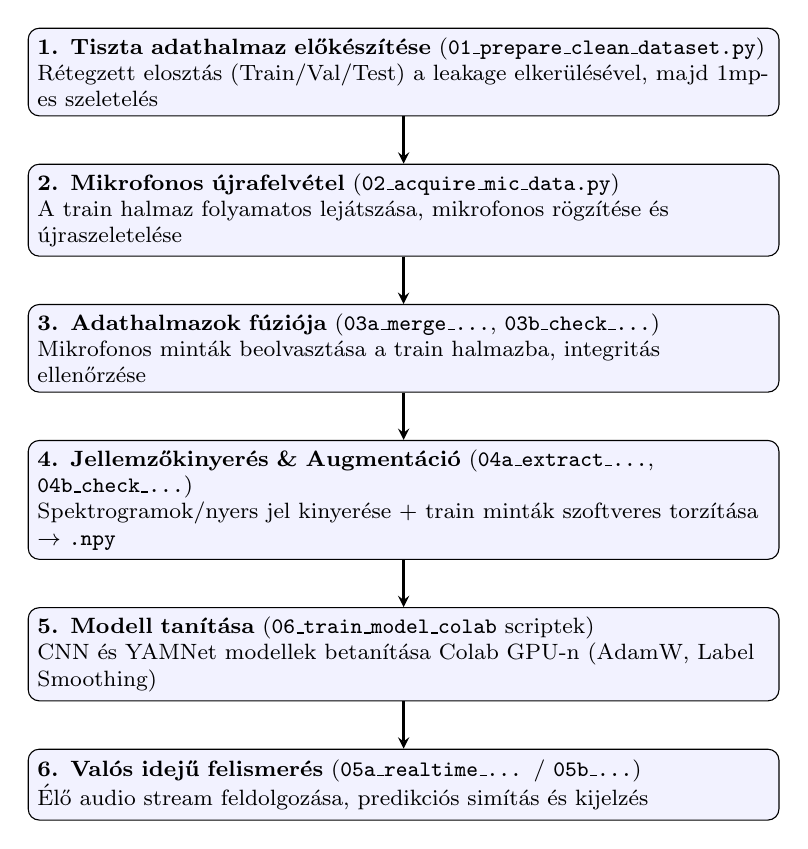
\begin{tikzpicture}[
    node distance=0.6cm,
    flowstep/.style={draw, rectangle, minimum height=0.9cm, minimum width=9.5cm, fill=blue!5!white, align=left, font=\footnotesize, rounded corners, text width=9.3cm},
    arrow/.style={thick,->,>=stealth}
]
  % Nodes
  \node (s1) [flowstep] {\textbf{1. Tiszta adathalmaz előkészítése} (\texttt{01\_prepare\_clean\_dataset.py}) \\ Rétegzett elosztás (Train/Val/Test) a leakage elkerülésével, majd 1mp-es szeletelés};
  
  \node (s2) [flowstep, below=of s1] {\textbf{2. Mikrofonos újrafelvétel} (\texttt{02\_acquire\_mic\_data.py}) \\ A train halmaz folyamatos lejátszása, mikrofonos rögzítése és újraszeletelése};
  
  \node (s3) [flowstep, below=of s2] {\textbf{3. Adathalmazok fúziója} (\texttt{03a\_merge\_...}, \texttt{03b\_check\_...}) \\ Mikrofonos minták beolvasztása a train halmazba, integritás ellenőrzése};
  
  \node (s4) [flowstep, below=of s3] {\textbf{4. Jellemzőkinyerés \& Augmentáció} (\texttt{04a\_extract\_...}, \texttt{04b\_check\_...}) \\ Spektrogramok/nyers jel kinyerése + train minták szoftveres torzítása $\rightarrow$ \texttt{.npy}};
  
  \node (s5) [flowstep, below=of s4] {\textbf{5. Modell tanítása} (\texttt{06\_train\_model\_colab} scriptek) \\ CNN és YAMNet modellek betanítása Colab GPU-n (AdamW, Label Smoothing)};
  
  \node (s6) [flowstep, below=of s5] {\textbf{6. Valós idejű felismerés} (\texttt{05a\_realtime\_...} / \texttt{05b\_...}) \\ Élő audio stream feldolgozása, predikciós simítás és kijelzés};

  % Arrows
  \draw [arrow] (s1) -- (s2);
  \draw [arrow] (s2) -- (s3);
  \draw [arrow] (s3) -- (s4);
  \draw [arrow] (s4) -- (s5);
  \draw [arrow] (s5) -- (s6);
\end{tikzpicture}
\caption{A hangszerfelismerő rendszer végső adatfeldolgozási és tanítási folyamatának lépései}
\label{fig:full_pipeline}
\end{figure}


\chapter{Üzembe helyezés és kísérleti eredmények}
\label{chap:uzembehelyezes}

Ez a fejezet bemutatja a rendszer üzembe helyezésének gyakorlati lépéseit, a szoftver fejlesztése és futtatása során felmerült technikai problémákat és azok megoldásait, valamint a betanított modellekkel végzett kísérletek és mérések számszerűsített eredményeit.

\section{Üzembe helyezési lépések}
\label{sec:uzembehelyezes}

A hangszerfelismerő rendszer két fő részből áll: a háttérben futó gépi tanulási és jelfeldolgozó modulokból, valamint a valós idejű parancssori felhasználói alkalmazásból (CLI Dashboard). A szoftver üzembe helyezéséhez az alábbi lépések szükségesek:

\begin{enumerate}
    \item \textbf{Python környezet előkészítése:} A futtatáshoz legalább Python 3.10 verzió szükséges. Ajánlott egy izolált virtuális környezet (virtual environment) létrehozása a függőségek kezelésére:
\begin{verbatim}
python3 -m venv venv
source venv/bin/activate
\end{verbatim}

    \item \textbf{Rendszerszintű függőségek telepítése:} A valós idejű hangrögzítésért felelős \texttt{sounddevice} könyvtár a PortAudio C-könyvtárra épül. macOS rendszereken ezt a Homebrew segítségével kell telepíteni:
\begin{verbatim}
brew install portaudio
\end{verbatim}
    Windows és Linux platformokon a csomagkezelők többsége automatikusan fordítja vagy tartalmazza a szükséges binárisokat.

    \item \textbf{Python könyvtárak telepítése:} A szükséges csomagok listáját a \texttt{requirements.txt} tartalmazza. Telepítésük a következő paranccsal végezhető el:
\begin{verbatim}
pip install -r requirements.txt
\end{verbatim}
    A legfontosabb telepített csomagok: \texttt{tensorflow} (neurális hálózat futtatása), \texttt{librosa} (jellemzőkinyerés), \texttt{sounddevice} (mikrofonkezelés), valamint a vizualizációért felelős \texttt{matplotlib} és \texttt{numpy}.

    \item \textbf{Modellfájlok elhelyezése:} A betanított neurális hálózati modelleket a \texttt{best\_log\_mel\_}\allowbreak\texttt{2dcnn\_model.keras} és a \texttt{best\_stft\_}\allowbreak\texttt{2dcnn\_model.keras} fájlok formájában a projekt \texttt{models/} alkönyvtárába kell elhelyezni.

    \textbf{}
    \item \textbf{Alkalmazás indítása:} A valós idejű parancssori felület az alábbi parancs futtatásával indítható el:
\begin{verbatim}
python scripts/07_realtime_recognition.py
\end{verbatim}
\end{enumerate}

\section{Felmerült problémák és megoldások}
\label{sec:problemak}

\section{Kísérleti eredmények és mérések}
\label{sec:kiserletek}

A legjobb eredményt nyújtó Log-Mel alapú modell hangszerenkénti osztályozási mátrixát (konfúziós mátrix) vizsgáltam meg részletesebben. A~\ref{fig:confusion_matrix}.~ábra hőtérkép (heatmap) formájában mutatja a hangszerosztályok közötti tévesztési arányokat és a pontos mintaszámokat az osztályozás során.

\begin{figure}[H]
  \centering
  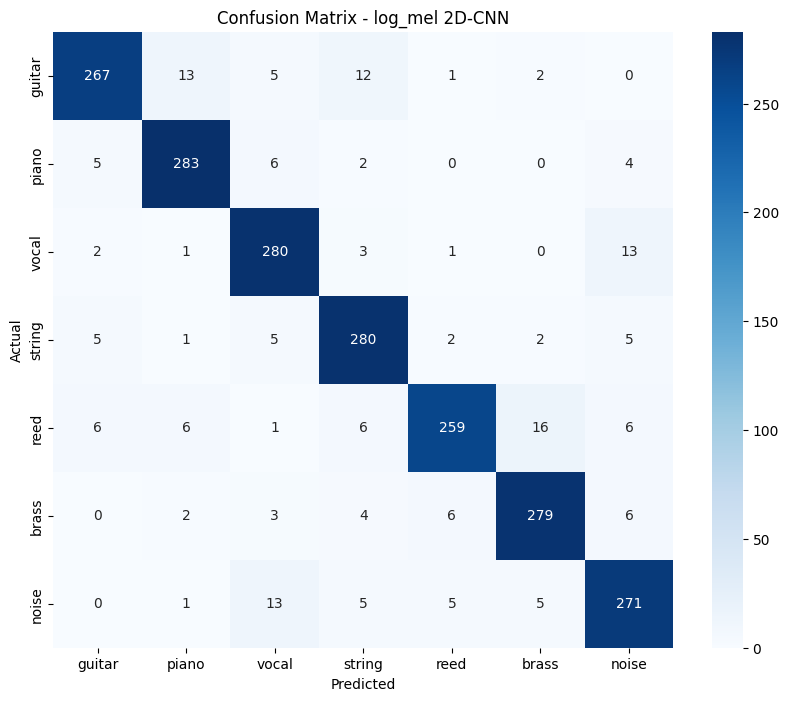
\includegraphics[width=0.8\textwidth]{fig_confusion_matrix.png}
  \caption{A Log-Mel spektrogram alapú 2D CNN modell konfúziós mátrixának hőtérképe}
  \label{fig:confusion_matrix}
\end{figure}

A konfúziós mátrix hőtérképéből leolvasható, hogy a legkönnyebben és legbiztosabban felismerhető kategória a \texttt{Zongora} (94,3\%, azaz 283 helyes predikció a 300 tesztmintából), valamint az \texttt{Ének} és a \texttt{Vonósok} (mindkettő 93,3\%, azaz 280/300 helyes osztályozás). A zongora tiszta leütési tranziensei és a vonósok egyenletes, hosszan tartó harmonikus felhangszerkezete jól elkülöníthető vizuális mintázatot adnak a Log-Mel spektrogramon, miközben az énekhang egyedi formánsai (a vokális traktus rezonanciája) szintén markáns ujjlenyomatként jelennek meg.

A legnagyobb arányú tévesztések a következők szerint alakultak:
\begin{itemize}
    \item \textbf{Fúvós hangszerek:} A \texttt{Nádas} fúvósok mintáinak 5,3\%-át (16 mintát) a modell \texttt{Rézfúvósnak} osztályozta. Ez a tévesztés akusztikailag rendkívül indokolt, mivel például az egynádas szaxofon (nádas fúvós) és a trombita (rézfúvós) felhangszerkezete és megszólalási tranziensei bizonyos hangmagasságoknál nagyon hasonlóak.
    \item \textbf{Zongora és Gitár:} A \texttt{Gitár} minták 4,3\%-át (13 mintát) a modell \texttt{Zongorának} osztályozta. Ez a pengetett és leütött húrok fizikai rezgésének kezdeti lecsengési hasonlóságából fakad, különösen az akusztikus gitár esetében.
    \item \textbf{Ének és Háttérzaj:} A \texttt{Háttérzaj} minták 4,3\%-át (13 mintát) \texttt{Éneknek}, míg az \texttt{Ének} minták 4,3\%-át (13 mintát) \texttt{Háttérzajnak} jelölte a hálózat. Ez a mikrofonos zörejek, zihálások és az emberi beszéd/ének frekvenciatartományának átfedései miatt fordul elő, valamint a halkabb énekszakaszok és a környezeti zajok hasonlóságából adódik.
\end{itemize}
Mintent összevetve a Log-Mel alapú 2D CNN modell kiválóan teljesít: a legnehezebbnek bizonyuló \texttt{Nádas} osztályban is eléri a 86,3\%-os pontosságot, míg a többi zenei és környezeti kategóriában 89\% feletti egyedi pontosságot biztosít.


\chapter{A rendszer felhasználása}
\label{chap:felhasznalas}

Ez a fejezet az elkészült hangszerfelismerő rendszer gyakorlati alkalmazását mutatja be a végfelhasználó szempontjából. Részletesen ismertetem a szoftver indításának menetét, a terminál alapú interaktív felhasználói felület (CLI Dashboard) felépítését és színkódolását, valamint bemutatok több tipikus valós idejű működési forgatókönyvet (tesztesetet) szöveges konzol-mockupokon keresztül.

\section{Az alkalmazás indítása és konfigurációja}
\label{sec:inditas}

A rendszer tervezése során kiemelt szempont volt a könnyű hordozhatóság és az alacsony erőforrás-igény. Mivel a szoftver egy interaktív, valós idejű parancssori felületen fut, nincs szükség erőforrás-igényes grafikus ablakkezelő rendszerek betöltésére, így az alkalmazás akár szervereken vagy korlátozott teljesítményű beágyazott eszközökön is futtatható.

Az indítás előfeltételei az alábbiak:
\begin{enumerate}
    \item A virtuális környezet aktiválása a projekt gyökérkönyvtárában:
\begin{lstlisting}
source venv/bin/activate
\end{lstlisting}
    \item A külső mikrofon vagy a beépített hangbemeneti eszköz csatlakoztatása és alapértelmezetté tétele a rendszerbeállításokban.
\end{enumerate}

Az indítás a következő parancs futtatásával történik:
\begin{lstlisting}
python scripts/05a_realtime_recognition.py
\end{lstlisting}

Az alkalmazás indításakor a konzolon megjelennek a konfigurációs paraméterek, a betanított Keras modell betöltésének állapota, valamint az élő jelfeldolgozási folyamat megkezdését jelző üzenet (lásd a \ref{fig:realtime_setup}.~ábrát):

\begin{figure}[H]
    \centering
    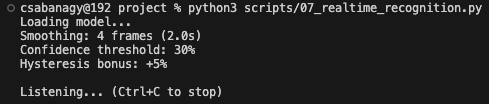
\includegraphics[width=0.75\textwidth]{fig_realtime_setup.png}
    \caption{Az alkalmazás indításakor megjelenő konfigurációs és betöltési paraméterek}
    \label{fig:realtime_setup}
\end{figure}

\section{A parancssori felhasználói felület felépítése}
\label{sec:cli_dashboard}

A valós idejű visszajelzést egy dinamikusan frissülő terminálsor (CLI Dashboard) biztosítja. A hagyományos, soronként görgető konzolos kiírás helyett a program a kocsivissza (\texttt{\textbackslash r}) karaktert használja, így a terminál egyetlen sorát írja felül folyamatosan a legfrissebb információkkal. Ez reszponzív, villódzásmentes felhasználói élményt nyújt.

A kijelző sor három fő vizuális komponensből áll:
\begin{enumerate}
    \item \textbf{Dinamikus konfidencia-sáv:} Egy 20 karakter hosszúságú grafikus sáv, amely a felismert hangszer valószínűségét ábrázolja vizuálisan. 
    \item \textbf{Aktív osztály és konfidencia érték:} A felismert hangszer megnevezése és a kiszámított valószínűségi százalékos érték (tizedes pontossággal). A kijelzőn látható aktív kategória csak akkor vált át egy új hangszerre vagy csendre, ha annak simított valószínűsége a háttérben meghaladja a beépített biztonsági küszöbértéket (hangszerek esetén $45\%$, zaj/csend esetén $20\%$). Ezzel biztosítja a program a stabil vizuális visszajelzést.
    \item \textbf{Másodlagos osztályok valószínűségei:} A többi hangszerosztály rövidített jelölése (G: Gitár, P: Zongora, V: Vokál, S: Vonós, R: Nádfúvós, B: Rézfúvós, N: Zaj/Csend) és azok pillanatnyi valószínűségi értékei, amelyek segítenek a felhasználónak átlátni a modell bizonytalansági tényezőit és az átfedéseket.
\end{enumerate}

\subsection{ANSI színkódolás és jelölések}

A felület a terminál ANSI escape szekvenciáit kihasználva színesben jeleníti meg a felismert hangszereket. Minden hangszerosztály egyedi, kontrasztos színt kapott, így a felhasználó akár távolabbról, a szöveg elolvasása nélkül is azonnal látja az aktív hangszert. A színkódokat, jelöléseket és az osztályok leírását a \ref{tab:ansi_colors}.~táblázat foglalja össze:

\begin{table}[H]
\centering
\caption{A parancssori felületen alkalmazott ANSI színkódok és rövidítések kategóriánként}
\label{tab:ansi_colors}
\begin{tabular}{llcl}
\toprule
\textbf{Kategória} & \textbf{Terminál színe} & \textbf{Rövidítés} & \textbf{Leírás} \\
\midrule
\texttt{guitar} & Sárga & G & Pengetős hangszerek (pl. akusztikus gitár) \\
\texttt{piano} & Inverz Fekete/Fehér & P & Billentyűs hangszerek (zongora) \\
\texttt{vocal} & Ciánkék & V & Emberi énekhang (vokál) \\
\texttt{string} & Sötétvörös & S & Vonós hangszerek \\
\texttt{reed} & Narancssárga & R & Nádas fúvós hangszerek (szaxofon) \\
\texttt{brass} & Világosbarna & B & Rézfúvós hangszerek \\
\texttt{noise} & Szürke & N & Környezeti zaj / csend \\
\bottomrule
\end{tabular}
\end{table}

\section{Működési forgatókönyvek és tesztesetek}
\label{sec:forgatokonyvek}

Az alábbiakban bemutatom, hogyan reagál a konzolos interfész a különböző akusztikai bemenetekre valós időben.

\subsection{1. teszteset: Csendes szobai környezet (alapállapot)}
Amikor a szobában nincs aktív hangszeres játék, csak a számítógép ventilátora vagy távoli környezeti zörejek hallatszanak, az RMS zajkapu átengedi a jelet (vagy a modell zajként azonosítja), így a szürke színű \texttt{noise} osztály válik aktívvá kiugróan magas konfidenciával. A terminál kijelzése ekkor a \ref{fig:realtime_noise}.~ábrán látható:

\begin{figure}[H]
    \centering
    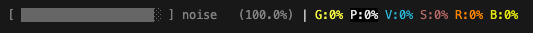
\includegraphics[width=0.6\textwidth]{fig_realtime_noise.png}
    \caption{A rendszer kimenete csendes szobai környezet (zaj) esetén}
    \label{fig:realtime_noise}
\end{figure}

\subsection{2. teszteset: Akusztikus gitárjáték (monofón dallam)}
Amikor a felhasználó megszólaltat egy akusztikus gitárt a mikrofon közelében, a modell az első ablak után azonnal reagál. A simító ablaknak ($2,0$ másodperc) és a hiszterézisnek köszönhetően a kijelzés stabilan átvált sárga színű \texttt{guitar} feliratra, miközben a többi hangszer valószínűsége minimálisra csökken (lásd a \ref{fig:realtime_guitar}.~ábrát):

\begin{figure}[H]
    \centering
    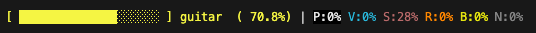
\includegraphics[width=0.6\textwidth]{fig_realtime_guitar.png}
    \caption{A rendszer kimenete akusztikus gitárjáték érzékelésekor}
    \label{fig:realtime_guitar}
\end{figure}

\subsection{3. teszteset: Emberi énekhang (vokál)}
Amikor a felhasználó énekelni vagy beszélni kezd a mikrofonba, a kijelző azonnal ciánkékre vált, és a \texttt{vocal} osztály jelenik meg. Mivel az ének felhangjai nagyon tiszták és erősek, a konfidencia érték gyorsan emelkedik (lásd a \ref{fig:realtime_vocal}.~ábrát):

\begin{figure}[H]
    \centering
    
\includegraphics[width=0.6\textwidth]{fig_realtime_vocal.png}
    \caption{A rendszer kimenete emberi énekhang (vokál) érzékelésekor}
    \label{fig:realtime_vocal}
\end{figure}

\subsection{4. teszteset: Szaxofon játék (átmeneti bizonytalanság)}
Amikor a felhasználó szaxofonon játszik, a modell kezdetben a rézfúvós és nádfúvós osztályok között oszcillálhat az akusztikai hasonlóságok miatt. A hiszterézis bónusz és a konfidencia-küszöb azonban stabilizálja az eredményt, így a kijelző fixen narancssárga \texttt{reed} színben marad (lásd a \ref{fig:realtime_reed}.~ábrát):

\begin{figure}[H]
    \centering
    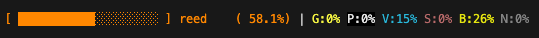
\includegraphics[width=0.6\textwidth]{fig_realtime_reed.png}
    \caption{A rendszer kimenete szaxofon játék (reed) érzékelésekor}
    \label{fig:realtime_reed}
\end{figure}

\subsection{Az alkalmazás leállítása}
A felhasználó bármikor megszakíthatja az élő elemzést a terminálban kiadott \texttt{Ctrl+C} billentyűkombinációval. Ekkor a parancssori visszahívási szálak lezárulnak, a mikrofonbemenet felszabadul, és a program tiszta állapotban kilép a terminálba, egy rövid \texttt{Stopped.} üzenet kíséretében.


\chapter{Következtetések}

A dolgozat végére érve a célom nem egy rekordpontosságú, minden helyzetben
hibátlan hangszerfelismerő rendszer bemutatása volt, hanem egy végigvezetett,
mérhető és valós időben is kipróbálható mérnöki prototípus elkészítése. Ebben
a fejezetben ezért röviden összefoglalom, mit valósítottam meg, hogyan
viszonyul a rendszer a hasonló megközelítésekhez, és merre lehetne továbbvinni
a munkát.

\section{Megvalósítások}
Megtervezni és megközelíteni egy, a cél szempontjából tökéletes, alacsony mintaszámú zenei adathalmazt szinte lehetetlen. Azonban egy igazán jót is kihívás, nem beszélve az osztályozó modell és a jellemzőkinyerő megválasztásáról és integrálásáról. Számomra igazi kihívást jelentett a rendszer élesítése. Már csak a minták kiválogatása alatt rengeteg szép hangszeres játékkal találtam szemben magam, ami csak emelte a munka iránti ambíciómat. Bár egy ilyen projekt sosincs kész, mindig van, amit javítani rajta, az eredmény minden kisebb-nagyobb hibája ellenére elégedettséggel tölt el, és büszkén foglal helyet a portfóliómban.

A munka során elért legfontosabb elméleti és gyakorlati megvalósítások az alábbi pontokban foglalhatók össze:
\begin{itemize}
    \item Egy olyan hibrid adathalmaz létrehozása és pontos struktúrájának kialakítása, amely egyszerű módon, bárki által újra felhasználható és bővíthető más hangszerfelismerési kutatásokban is.
    \item Egy moduláris feldolgozási csővezeték kiépítése, amely lehetővé teszi a különböző jellemzőkinyerési eljárások (STFT, Log-Mel, MFCC) és modellek könnyű cseréjét a rendszerben.
    \item Az egyszerű, offline (fájl alapú) osztályozáson túl egy olyan valós idejű hangszerfelismerő alkalmazás megvalósítása, amely közvetlen mikrofon-bemenetet használ.
    \item A valós idejű predikciót simító és stabilizáló logika implementálása (mozgóátlag-számítás), amely megbízhatóbbá és gördülékenyebbé teszi a kijelzést.
    \item A 2D CNN modell optimalizálása a gyorsabb és alacsonyabb késleltetésű futás elérése érdekében, biztosítva a zökkenőmentes kiértékelést egy átlagos asztali számítógépen.
\end{itemize}

\section{Hasonló rendszerekkel való összehasonlítás}
A \ref{sec:hasonlo_alkalmazasok}.~szakaszban bemutatott kapcsolódó munkákhoz képest a saját rendszerem nem a legnagyobb lehetséges adathalmazt vagy a legerősebb neurális architektúrát célozta meg. A szakirodalomban gyakoriak a nagyobb, polifón zenei anyagokra épülő rendszerek, illetve az olyan előtanított vagy mélyebb modellek, amelyek erős általánosító képességet adhatnak, de a fejlesztési és futtatási környezetük is összetettebb. Ezzel szemben én egy kisebb, átláthatóbb, saját adatgyűjtésre épülő rendszert készítettem, ahol a módszertani kérdések -- például az augmentáció, a mikrofonos domain shift és a végső testelés -- kézben tarthatók és védhetően dokumentálhatók.

A saját Log-Mel + 2D CNN modell legfontosabb előnye nem az, hogy minden mérőszámban felülmúlja a transfer learning megközelítést, hanem az, hogy teljes feldolgozási láncként saját kézben van: a hanggyűjtéstől a jellemzőkinyerésen át a valós idejű predikcióig. A YAMNet-alapú összehasonlítás megmutatta, hogy az előtanított embedding erősebb kiindulópont lehet, de a saját modell is értelmezhető, futtatható és a dolgozat céljához illeszkedő megoldást ad. A rendszer tehát nem ipari szintű, általános hangszerfelismerő szolgáltatásként értékelendő, hanem egy BSc szintű, végigvezetett mérnöki prototípusként, amelyben a döntések és a korlátok is világosan követhetők.

\section{Továbbfejlesztési lehetőségek}
A rendszerben számtalan továbbfejlesztési lehetőség adott. Elsősorban a kutatás továbbvihető a zajos monofón felismeréstől a tiszta polifón hangszerfelismerés irányába. Ebben az esetben a meglévő softmax aktivációs függvényt sigmoidra kellene cserélnünk a kimeneti rétegen, és többcímkés (multi-label) osztályozást kellene alkalmaznunk, hiszen egyszerre több hangszer is megszólalhat. Ehhez azonban az eddiginél még sokkal több adatra lenne szükség, amelyet szintén az internetről gyűjthet össze az ember, vagy mesterségesen, két különálló hangszer hangját egy szkript segítségével összekeverve állíthat elő.

Ha még nagyobb kihívásra vágyik valaki, el lehet merészkedni a nagy, zajos zenekarokig (orchesztrákig), amelyek a jelen kiváló mérnökeinek is komoly fejtörést okoznak. Minden fejlesztés alapja először úgyis egy stabil és megbízható adathalmaz létrehozása.

Amennyiben a koncepcióval nem a zene felé, hanem egy iparibb környezet irányába indulnánk el, az adathalmaz átszervezésével készíthető egy ipari gépek állapotát felmérő szenzor is. Ez képes lenne megmondani a hang alapján, ha például egy gépből fogyóban van a kenőolaj, ha életlenné vált egy körfűrész (cirkula), vagy egyéb, az ipari gépek állapotával kapcsolatos előrejelzéseket adhatna.


% ════════════════════════════════════════════════════════════════════════════
% BIBLIOGRAPHY
% ════════════════════════════════════════════════════════════════════════════
\nocite{*}
\printbibliography[title={Irodalomjegyzék}, heading=bibintoc]

% ════════════════════════════════════════════════════════════════════════════
% APPENDICES
% ════════════════════════════════════════════════════════════════════════════
\appendix

\chapter{Függelékek}
\label{chap:fuggelek}

A függelék tartalmazza az „Automatikus hangszerfelismerés zenefelvételek alapján” című államvizsga-szakdolgozat teljes forráskódját, az adathalmaz-struktúrát és a betanított modellfájlokat tartalmazó digitális adathordozó könyvtárszerkezetének leírását, valamint a felhasznált szoftverfüggőségek összegzését.

%% ═══════════════════════════════════════════════════════════════════════════
\section{A projekt könyvtárszerkezete}
\label{sec:konyvtarszerkezet}

A benyújtott digitális függelék (amely a GitHubon elérhető nyilvános Git adattárban\footnote{\url{https://github.com/nCsab/Instrument-Recognition}} is megtalálható) az alábbi főbb könyvtárakat tartalmazza. A számozott szkriptek a feldolgozási csővezeték (pipeline) egymásra épülő lépéseit jelzik.

\begin{table}[ht!]
\centering
\small
\caption{A projekt legfelső szintű könyvtárszerkezete}
\label{tab:konyvtarszerkezet}
\begin{tabular}{p{4.5cm}p{10cm}}
\toprule
\textbf{Könyvtár / Fájl} & \textbf{Leírás} \\
\midrule
\texttt{thesis/} & A \LaTeX\ formátumú szakdolgozat forrásfájljai, stílusfájl (\texttt{sapientia-thesis.cls}), irodalomjegyzék (\texttt{references.bib}) és a generált \texttt{main.pdf}. \\
\texttt{scripts/} & A hangszerfelismerő rendszer Python szkriptjei (részletezés alább). \\
\texttt{owndataset/} & A manuálisan összeválogatott és kivágott internetes hangminták hangszerosztályonként külön almappákban, valamint az újrafelvételezett minták a \texttt{recorded\_from\_mic/} almappában. \\
\texttt{hybrid\_dataset\_\allowbreak own\_final/} & A végleges, összeszerelt hibrid adathalmaz 7~osztálymappával (\texttt{guitar}, \texttt{piano}, \texttt{vocal}, \texttt{string}, \texttt{reed}, \texttt{brass}, \texttt{noise}), osztályonként 1500~db, 1~másodperces, 16\,kHz-es WAV minta. \\
\texttt{processed\_data/} & Az előállított jellemzőmátrixok NumPy formátumban: \texttt{X\_stft\_full.npy}, \texttt{X\_log\_mel\_full.npy}, \texttt{X\_mfcc\_full.npy} és a közös címkefájl \texttt{y\_labels\_full.npy}. \\
\texttt{models/} & A betanított Keras modellfájlok: \texttt{best\_stft\_2dcnn\_model.keras}, \texttt{best\_log\_mel\_2dcnn\_model.keras}, \texttt{best\_mfcc\_2dcnn\_model.keras}. \\
\texttt{augmented\_samples/} & Az augmentációs lánc bemutató mintái: minden hangszerosztályból 3-3 eredeti--augmentált páros WAV fájl ellenőrzés céljából. \\
\texttt{dataset/} & A letöltött nyilvános referencia-adathalmazok (IRMAS, NSynth, Medley-solos-DB, TinySOL, Good-sounds, ESC-50) az elemzéshez. \\
\bottomrule
\end{tabular}
\end{table}
\clearpage
%% ═══════════════════════════════════════════════════════════════════════════
\section{A feldolgozási csővezeték szkriptjei}
\label{sec:pipeline_scripts}

A rendszer teljes feldolgozási lánca indexelt Python szkriptekből áll, amelyek a tervezés sorrendjében futtathatók. Az alábbi táblázat leírja minden szkript feladatát.

\begin{table}[ht!]
\centering
\small
\caption{A feldolgozási csővezeték szkriptjei és feladataik}
\label{tab:pipeline_scripts}
\begin{tabular}{p{5.8cm}p{8.7cm}}
\toprule
\textbf{Szkript} & \textbf{Feladat} \\
\midrule
\texttt{01\_analyze\_datasets.py} & A nyilvános referencia-adathalmazok (IRMAS, NSynth stb.) szerkezetének és statisztikáinak feltárása, összehasonlító elemzés készítése. \\
\texttt{02\_mic\_prep\_\allowbreak concatenate.py} & Az újrafelvételezéshez szükséges hanganyag előkészítése: a kiválasztott minták összefűzése egyetlen hosszú WAV fájlba sípszó-szinkronizálással. \\
\texttt{03\_mic\_record\_audio.py} & A laptop beépített mikrofonjával vagy mobiltelefon mikrofonjával történő visszajátszás és valós idejű rögzítés. \\
\texttt{04\_mic\_slice\_audio.py} & A rögzített mikrofonos felvétel darabolása 1~másodperces szegmensekre a sípszó-szinkronizáció alapján. \\
\texttt{05\_assemble\_dataset.py} & A végleges hibrid adathalmaz összeállítása: a tiszta minták, az újrafelvételek és az augmentált minták egyesítése és randomizált másolása a \texttt{hybrid\_dataset\_own\_final/} könyvtárba. \\
\texttt{05a\_prepare\_hybrid\_\allowbreak generic.py} & Kiegészítő előkészítő szkript a hibrid adathalmaz generikus felépítéséhez. \\
\texttt{06\_extract\_features.py} & A fő jellemzőkinyerő szkript, amely az összes hangmintából STFT, log-mel és MFCC spektrogramokat generál, és NumPy mátrixokba menti. \\
\texttt{06\_extract\_features/} & Alkönyvtár a három jellemzőtípus önálló kinyerő szkriptjeivel: \texttt{06\_extract\_stft.py}, \texttt{06\_extract\_log\_mel.py}, \texttt{06\_extract\_mfcc.py}. \\
\texttt{07\_realtime\_\allowbreak recognition.py} & A valós idejű hangszerfelismerő modul: mikrofon-bemenet, csúszóablak, előrejelzés és megjelenítés. \\
\texttt{10\_train\_model\_colab/} & A Google Colab felhőkörnyezetben futtatott tanító szkriptek: \texttt{10\_train\_stft.py}, \texttt{10\_train\_log\_mel.py}, \texttt{10\_train\_mfcc.py}. \\
\texttt{utils/} & Segédmodulok: \texttt{augmentation\_utils.py} (az augmentációs lánc függvényei) és \texttt{feature\_utils.py} (jellemzőkinyerési segédfüggvények). \\
\bottomrule
\end{tabular}
\end{table}

\clearpage
%% ═══════════════════════════════════════════════════════════════════════════
\section{Fejlesztői és futtatási környezet}
\label{sec:fejlesztoi_kornyezet}

Az alábbi táblázat tartalmazza a projekt fejlesztéséhez és futtatásához szükséges szoftverfüggőségeket.

\begin{table}[H]
\centering
\caption{A fejlesztői környezet főbb összetevői}
\label{tab:fejlesztoi_kornyezet}
\begin{tabular}{p{4.2cm}p{2.5cm}p{7.5cm}}
\toprule
\textbf{Szoftver / Könyvtár} & \textbf{Verzió} & \textbf{Felhasználás} \\
\midrule
Python & 3.10+ & A teljes feldolgozási csővezeték nyelve \\
\addlinespace
TensorFlow / Keras & 2.x & A 2D CNN modell építése, tanítása és mentése \\
\addlinespace
Librosa & 0.10+ & Hangfájlok betöltése, STFT, mel-spektrogram és MFCC kinyerés \\
\addlinespace
NumPy & 1.24+ & Jellemzőmátrixok tárolása és manipulálása \\
\addlinespace
SoundFile / SoundDevice & -- & Hangfájlok olvasása/írása és valós idejű mikrofon-hozzáférés \\
\addlinespace
Matplotlib & 3.x & Diagramok, spektrogramok és kiértékelési ábrák készítése \\
\addlinespace
Google Colab & -- & GPU-gyorsított modelltanítás felhőkörnyezetben \\
\addlinespace
Git & 2.x & Verziókezelés és a projekt előrehaladásának dokumentálása \\
\addlinespace
\LaTeX\ (TeX Live 2026) & -- & A szakdolgozat szedése a Sapientia sablon alapján \\
\bottomrule
\end{tabular}
\end{table}


\end{document}